\documentclass[11pt]{report}
% packages
\usepackage{baththesis}
\usepackage{amssymb} %for Blackboard bold etc
\usepackage{amsmath}
\usepackage{amsfonts}
\usepackage{graphicx} %for including eps graphics
\usepackage{float}
\usepackage[english]{babel}
\usepackage{placeins}

\usepackage{hyperref}

\usepackage{tikz}
\usepackage{wrapfig}
\usepackage{titlecaps}
\usepackage{sectsty}% http://ctan.org/pkg/sectsty

\usepackage{epstopdf}


%\usepackage[printwatermark]{xwatermark}
%\newsavebox\mybox
%\savebox\mybox{\tikz[color=red,opacity=0.3]\node{CONFIDENTIAL};}
%\newwatermark*[
%  allpages,
%  angle=45,
%  scale=6,
%  xpos=-20,
%  ypos=15
%]{\usebox\mybox}
%




\usepackage{algpseudocode,algorithm,algorithmicx}
\algrenewcommand\algorithmicrequire{\textbf{Launch:}}
%%%
\algrenewcommand\algorithmicensure{\textbf{End Kernel}}

\makeatletter
\def\ALG@special@indent{%
    \ifdim\ALG@thistlm=0pt\relax
        \hskip-\leftmargin
    \else
        \hskip\ALG@thistlm
    \fi
}
\newcommand{\Launch}[1]{\item[]\noindent\ALG@special@indent \textbf{Launch:}\ #1}
\newcommand{\EndKernel}{\item[]\noindent\ALG@special@indent \textbf{End Kernel}}
\makeatother

\usepackage{subfigure} 

\usepackage{indentfirst}
\usepackage{booktabs} % for much better looking tables
\usepackage{array} % for better arrays (eg matrices) in maths
\usepackage{paralist} % very flexible & customisable lists (eg. enumerate/itemize, etc.)
\usepackage{verbatim} % adds environment for commenting out blocks of text & for better verb
\usepackage{matlab-prettifier}
\renewcommand{\lstlistingname}{Code Snippet}
\usepackage{multicol}
\usepackage{caption}
\usepackage{makecell}

\newcommand{\argmin}{\mathop{\mathrm{arg\,min}}}
\newcommand{\argmax}{\mathop{\mathrm{arg\,max}}}


\makeatletter
\newcommand{\vast}{\bBigg@{4}}
\newcommand{\Vast}{\bBigg@{5}}
\makeatother






% front matter
\title{Motion compensation in X-ray tomography}
\author{Ander Biguri}
\degree{Doctor of Philosophy}
\department{Department of Electrical and Electronic Engineering}
\degreemonthyear{September 2017}
\norestrictions




\begin{document}
\maketitle

%\begin{abstract}
%bla
%\end{abstract}




\tableofcontents
\listoffigures
\listoftables

\begin{abstract}
Computed tomography (CT), and especially cone-beam computed tomography (CBCT) has a wide range of applications. This thesis focuses on CBCT for image-guided radiation therapy (IGRT), particularly for lung cancer treatment. In lung IGRT the tumour moves due to respiration, not only making it hard to target with the radiation beam, but also blurring the images acquired for daily treatment tuning. Generating high quality images without motion artefacts is essential for RT and hadron therapy. In this thesis, motion modelling ideas from CERNs proton synchrotron's phase space tomography are modified and adapted to lung CBCT. The CERN method includes a knowledge of the motion in the basic building blocks of the image reconstruction and uses all the acquired data to reconstruct a single static image at any chosen moment within the acquisition timespan. In order to use this method, and in general improve the reconstructed image quality of CBCT, iterative algorithms are explored with a focus on fast reconstruction using GPUs. The work presented here lead to the publication of the TIGRE Toolbox, a fast, easy-to-use MATLAB-CUDA toolbox for the reconstruction of CBCT images at state-of-the-art speeds with an extensive variety of iterative algorithms. This thesis presents the mathematics, GPU techniques and different applications of TIGRE and its algorithms, strengthening the idea already stated that iterative algorithms can significantly improve image quality in CBCT. A motion compensation method is developed together with a fast GPU implementation and its robustness is tested numerically by simulating the expected clinical errors in the data. The method is very robust and provides high-quality static images using data from disparate moments in time, offering the prospect of videos of patients breathing at no extra cost in radiation dose.

\end{abstract}

\chapterfont{\titlecap}
\sectionfont{\titlecap}
\subsectionfont{\titlecap}
\subsubsectionfont{\titlecap}

\Addlcwords{the on by in of and at from via}
%\chapter{X-ray imaging in medicine}
\chapter{Introduction and Motivation}\label{ch:intro}


Lung cancer is one of the most common \textcolor{blue}{cancers} in the world. It is the prevalent cancer type both in incidence and mortality in men and third in incidence and second in mortality, after breast cancer, in women\cite{WCR2014}. Death due to lung cancer surpass 1.5 million a year(see figure \ref{fig:world} for incidence), having around 10\% of five year survival rate in developed countries, and much lower in developing countries\cite{CRUK2014}. One in fourteen people has a lifetime risk of developing lung cancer\cite{Harrisons2012}, on average between men and women. The high incidence and mortality rates has lead to a high research throughput in mutidiciplinary fields, in order advance further the detection and treatment techniques of the disease, resulting in an output of over 23.000 lung cancer related research articles in reputable journals in the last 10 years\cite{Nature2015}. At the same time, the  actual lung cancer treatment has been transformed from non-existent in the 70s to being available worldwide\cite{Comis2003}.


\begin{figure}[ht]
\begin{center}
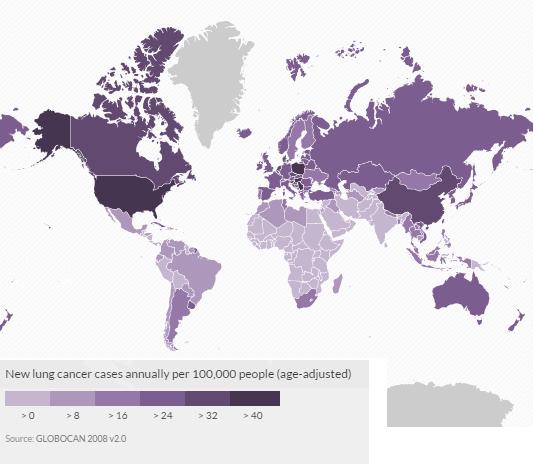
\includegraphics[width=0.65\columnwidth]{StateOfArt/worldmap.png}
\caption[Lung cancer incidence in the world]{Lung cancer incidence per country, age adjusted data. Map and data from {GLOBOCAN}\cite{GLOBOCAN2010}.}
%IARC has proprietary rights to the materials on the Website. Publications/data made available by IARC/WHO enjoy copyright protection in accordance with the provisions of Protocol 2 of the Universal Copyright Convention. All rights are reserved. Materials (fact sheets, maps, estimates or data) may be used "as is" for research, educational or other non-commercial purposes, but the corresponding reference must be cited in all cases.
\label{fig:world}
\end{center}
\end{figure}

Lung cancer treatment, while diverse between types of cancer, can be classified in four main types: chemotherapy, lobectomy or pneumoctomy, radiotherapy (RT) and palliative care. Generally, in early stages of small cell lung cancer the common treatment would consist in chemotherapy with radiotherapy, usually followed by brain radiotherapy, as there is a chance of metastasis in the brain. In the unlikely chance that the tumour is detected at a very early stage and has not spread to the lymph nodes, a lobectomy may be performed, removing part of the lung. Usually this is followed by radiotherapy and chemotherapy to make sure the tumour is completely removed.
In the case of non-small cell lung cancer, in the first stages the patient may undergo a lobectomy or a pneumoctomy (removal of the whole lung). Generally radiotherapy and chemotherapy (less likely) are added to the treatment in this case too. In the last stages of the lung cancer, usually the treatment is palliative care i.e. treatments to reduce the symptoms and relieve pain\cite{CRUK2014b}.

In practically all stages of different lung cancer treatments, radiotherapy is extensively used as above half of the treated patients do undergo the procedure\cite{Cancerorg}, with around 120,000 patients are treated with radiotherapy in the UK every year. Radiotherapy is a non-invasive technique that aims to destroy malignant cells using ionizing radiation, generally using photons. This is possible because high energy photons (X-rays) ionize the atoms that are part of the DNA chain, damaging it thus causing cellular death. In photon therapy, this happens due to the ionization of the water in the cells, that forms free radicals, such as hydroxyl radicals, destroying the DNA of the cells. Conventional photon RT is widely used around the world.

However, a different type of radiation therapy exists, particle therapy or hadron therapy, that uses charged particles instead of photons, by accelerating them with circular particle accelerators. These particles (protons and heavy ions)  penetrate the tissue with minimal interaction and release almost all the energy before stopping. Figure \ref{fig:bragg} shows the energy deposition (dose) plotted versus the penetration of the energy beam in tissue. The energy burst that hadrons show is referred to as the Bragg peak, after its discoverer William Henry Bragg. The Bragg peak allows for a radiation therapy where a larger amount of healthy tissue can be spared, while delivering highly spatially accurate doses to only the tumour areas. While the growth of hadron therapy has been slow in the past due to its cost, it is now being accelerated thanks to international collaboration projects such as ENLIGHT\cite{dosanjhparticle}, with 100 centres estimated by 2020 around the globe, 30 of them in Europe, 3 of them being already in their final stages in construction in the UK.

\begin{figure}[ht]
\begin{center}
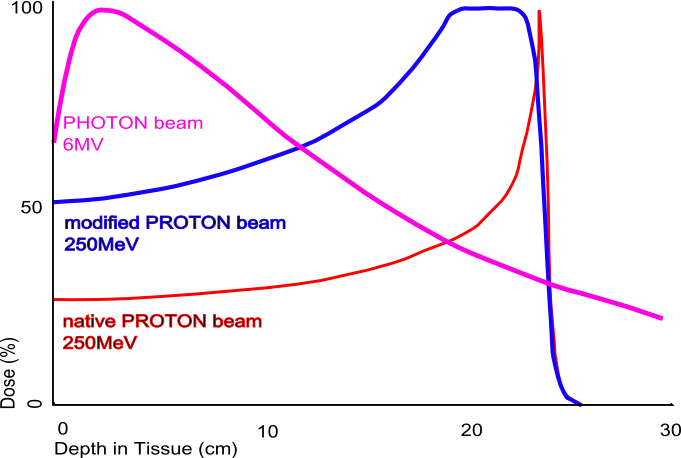
\includegraphics[width=0.6\columnwidth]{Introduction/BraggPeak.png}
\caption[Bragg peak]{ Depth-dose curves for photons (X rays) and protons (monoenergetic: red, polyenergetic:blue, indicating the different dose deposition behaviour of photons and charged particles when traversing matter. The ``spread-out Bragg peak'' can be tailored to provide a highly conformal dose deposit to the tumour volume, thus largely sparing surrounding healthy tissue from unwanted dose deposition. The proposal of  exploiting the favourable properties of heavy charged particles for cancer treatment was first proposed by Wilson\cite{wilson1946radiological}.}
%GNU license, wikipedia
\label{fig:bragg}
\end{center}
\end{figure}


RT treatment is nowadays generally guided by imaging systems during treatment planning (image guided radiation therapy, IGRT). Imaging systems, such as computed tomography (CT) and magnetic resonance imaging (MRI) are used to carefully tune the X-ray beam to focus in the specific location and shape of the tumour, and monitor the effects during the whole treatment period. Tumours not only are very different between patients, but also change considerably during treatment, so does the patient due to the physical toll of cancer treatment. This means that the tumour does change both shape and location and that, if these changes are not known, healthy tissue could be damaged and cancerous tissue spared. Generally, patients will be imaged before each treatment,  one of the most common systems for imaging being cone beam computed tomography (CBCT). CBCT takes several minutes to scan a patient due to mechanical safety limitations. As one can foresee, this is an important limiting factor for tumours that move, such as the liver and the lung ones, as the motion during acquisition can generate heavy artefacts around the moving parts in image reconstruction. This moving effect is also an important factor to be taken into account in hadron therapy, as having a moving tumour means a high chance of missing the treatment target. Providing accurate imaging not only in space, but also in time (4D imaging) is a key factor in treatment planning, \textcolor{blue}{and} thus in cancer treatment. Figure \ref{fig:motionblurr} shows the motion artefacts common in CBCT.

Interestingly, a motion compensation method for when objects are moving during \textcolor{blue}{acquisition} was proposed by Hancock \textit{et al}\cite{pst1}\cite{pst2}\cite{pstweb} for monitoring the phase space of high energy particle bunches in particle accelerators at CERN. Phase space tomography is a hybrid algorithm that combines particle tracking in a computer model of a synchrotron with iterative reconstruction algorithms to reconstruct an image of the population of a bunch of particles circulating in the accelerator. The particle motion involves \tb{a complex non-uniform rotation across the phase space} and is non-cyclic, but a 1D projection of the distribution can be completely acquired as a single snapshot \tb{on} one turn of the machine. By tracking test particles to gain a knowledge of how the geometry of the 2D image plane (longitudinal phase space) deforms, the information in all the discrete time slices acquired over many turns can be translated back to the same instant and tomographically combined in a single image.  Exploring the feasibility of using this tomographic motion compensation technique in medical applications is the objective of this thesis.

\begin{figure}

\begin{center} 
\subfigure[]{ 
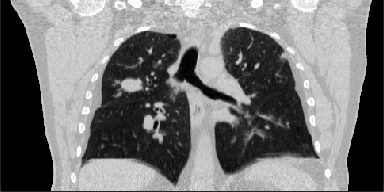
\includegraphics[width=0.4\linewidth]{Introduction/static.png} 
}
\subfigure[]{ 
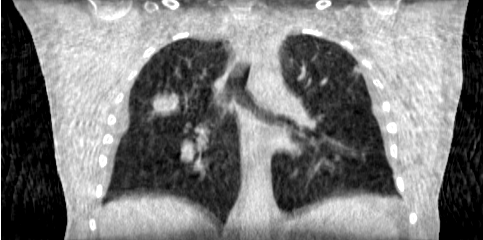
\includegraphics[width=0.4\linewidth]{Introduction/motionblur.png} 
}
 
\caption[Motion blurr in lung CBCT]{\label{fig:motionblurr}(a) Static CT image of a patient (from a 4D-CT dataset) (b) motion artefacts when reconstructed using data acquired from various breathing periods (simulated). The dataset is the POPI model\cite{popi-modelweb}.}
\end{center} 
\end{figure}


%% BLURRED IMAGE OF TUMOUR

\section{Aim of the thesis}

CBCT and computed tomography (CT) in general image reconstruction problem is a complex mathematical and computational challenge, even for just 3D spatial reconstruction, without the additional problem of motion. Mathematically CT reconstruction is an ill-posed problem and generally the volume to reconstruct is considerably larger than the data obtained, making the problem underdetermined. Often, an analytic approximated solution for the  mathematical problem is used, however this solution is considerably sensitive to noise and low amounts of data. As opposed to the analytic approximated solution, algebraic equation solving methods can be used. These generally lead to more robust solutions, especially with noisy and undersampled data. However, they require increased computational times, making them harder to introduce to clinical applications. There are two main research problems tackled in this work:

\begin{itemize}
\item Firstly, this thesis explores the image reconstruction problem, with a focus on implementing accurate iterative algorithms, and accelerating them as much as possible, using GPU technology. The results from this part of the thesis are applicable to any CT application, from the medical one, to industrial or research cases. The work here explores a variety of algorithms for CT reconstruction, with both mathematical and computational focus.
\item Secondly, the thesis concentrates on translating the motion compensation methods to the medical CBCT, focusing on \tb{lung} IGRT applications, focusing also on the computational side of the method, as well as its robustness.
\end{itemize}

All the research presented here has been made public as part of the TIGRE Toolbox\cite{TIGRE} and can be found in a GitHub repository\cite{TIGREweb} for both MATLAB and Python. 

\section{Thesis organization}

The chapters of this thesis try to be a self contained document. However, it can be separated into two main topics: GPU-based CT reconstruction (Chapters 3, 4 and 5) and motion compensation methods for IGRT (Chapters 2, 6 and 7). \tb{Chapter 8 concludes the thesis and proposes future work.} The contents of each chapter are summarized as follows:

\subsubsection{Chapter 2: Image Guided Radiation Therapy and Computed Tomography}


\begin{wrapfigure}{L}{0.35\textwidth}
\centering
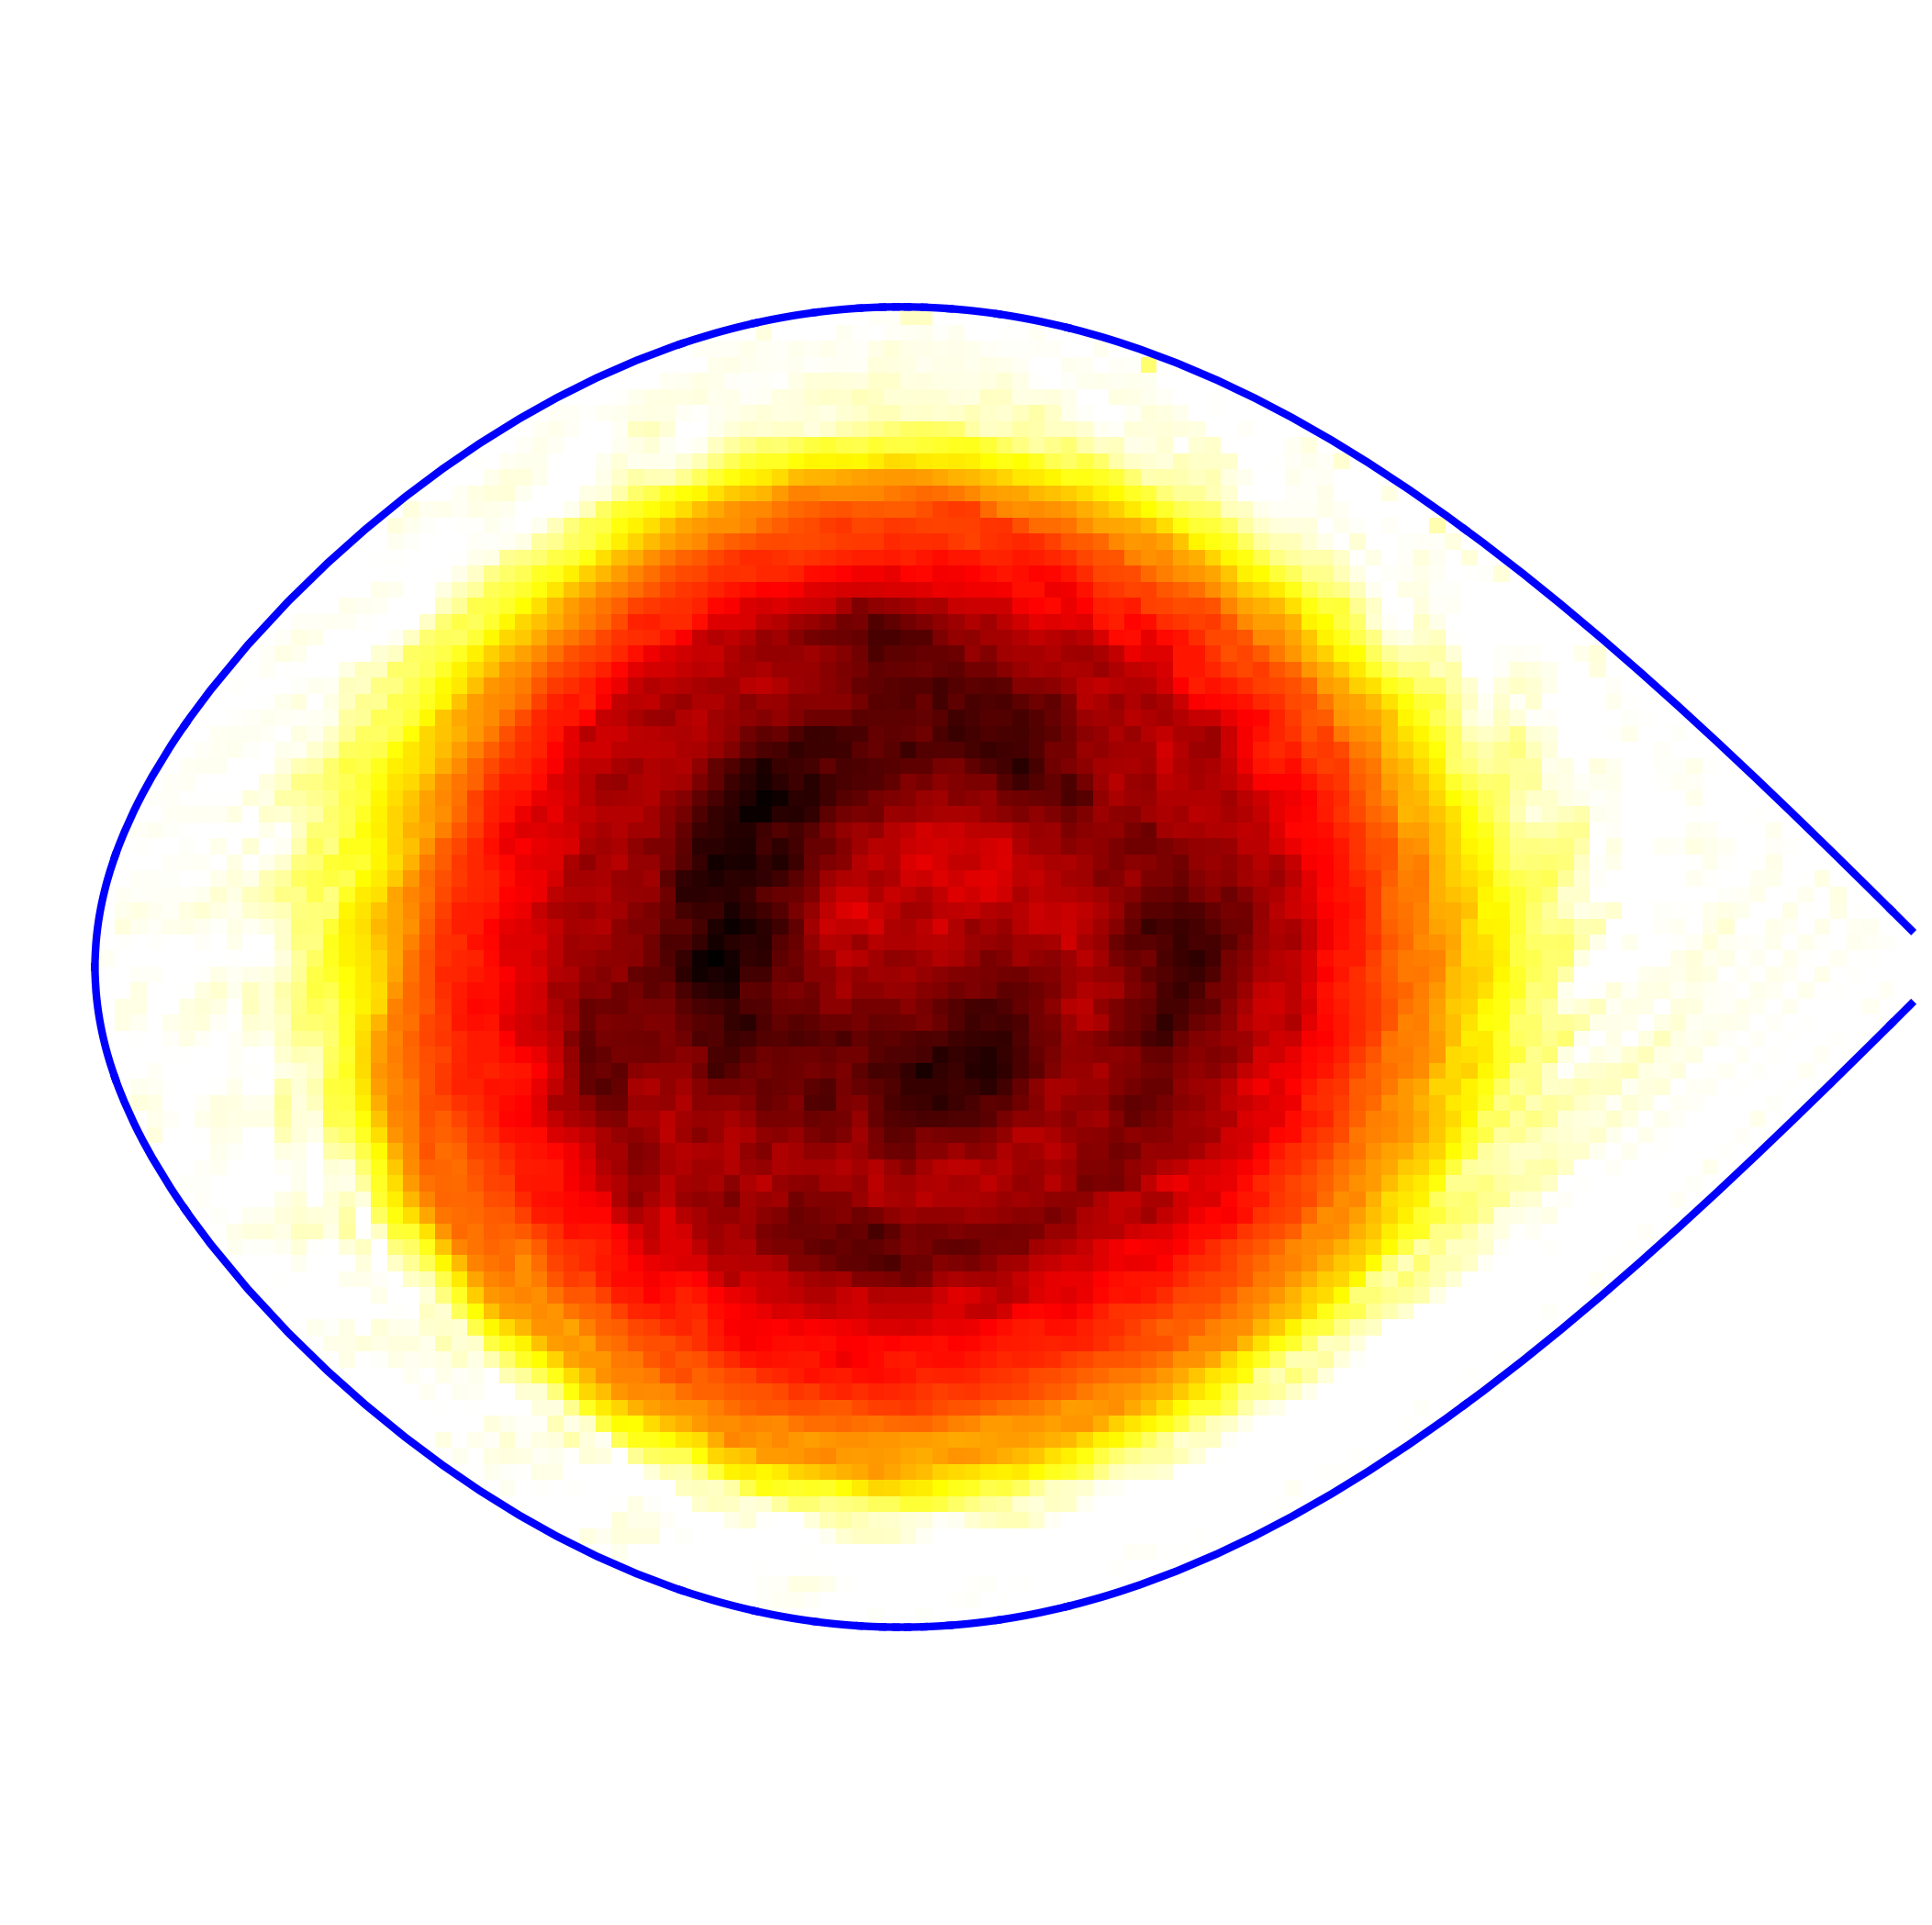
\includegraphics[width=0.32\textwidth]{StateOfArt/pst.png}
\end{wrapfigure}

An introduction to IGRT, focusing on imaging and the challenges in providing quality imaging for radiation treatment for both photon and hadron radiation therapy. As CBCT is one of the most widely used imaging systems for IGRT, a further study into the innovations of CBCT is presented, focusing after on the research available for dealing with non-rigid motion, such as respiratory motion. This exhaustive research shows that the vast majority of motion compensation algorithm are based on binning the data according to breathing phase and reconstructing an image for each bin, while very few publications exist with a similar concept for motion compensation as the phase space tomography, with no computational focus. Finally, there is a brief description of the wider uses of CT in general, from research to industry.

\vspace{40pt}
\subsubsection{Chapter 3: The Image Reconstruction Problem}

\begin{wrapfigure}{L}{0.35\textwidth}
\centering
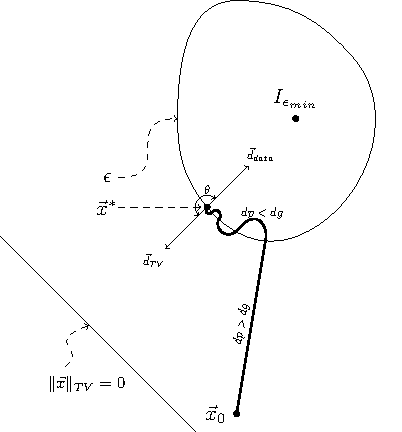
\includegraphics[width=0.32\textwidth]{RecAlgorithms/POCS.pdf}
\end{wrapfigure}

CBCT image reconstruction is an ill-posed problem, \tb{where even if solution may exists a stable numerical solution for it is not feasible\cite{Finch}}. Substandard conditions on the data acquisition process (such as noise, or geometric errors) and limited data can have a severe influence on the quality of the image reconstructed, especially using the Feldkamp Davis and Kress (FDK) method that approximates the analytic solution. However FDK is the most commonly used algorithm across the field. The reconstruction problem can however be described as an algebraic minimization problem, and iterative solvers can be used for minimization. This chapter describes briefly FDK and continues to showcase the mathematics of a variety of different iterative solvers for CBCT, such as SART and similar methods, Krylov subspace methods and a variety of total variation regularized iterative methods.
\FloatBarrier
\subsubsection{Chapter 4: GPU methods in tomography}



\begin{wrapfigure}{L}{0.35\textwidth}
\centering
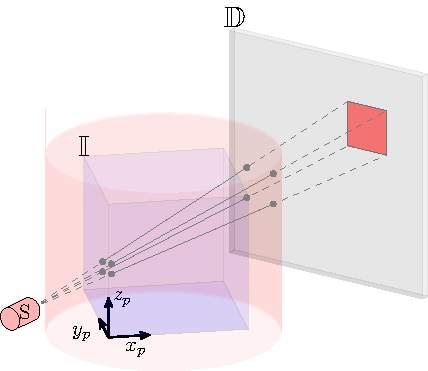
\includegraphics[width=0.32\textwidth]{GPUmethods/projcoord-figure0.pdf}
\end{wrapfigure}

CBCT reconstruction is a computationally very expensive problem. Iterative algorithms only enhance this problem, as they require sometimes hundreds of iterations, each of them being more costly than a single FDK solution. This chapter shows how GPU computing can accelerate the image reconstruction by tailoring very fast algorithms to GPU computational structure. It describes how the projection and backprojection operators (the basic building blocks of CT reconstruction) are implemented to reach state of the art speeds using different X-ray approximation methods. Finally, after showing how these have been used together with the mathematics of Chapter 3 to build the TIGRE Toolbox, an easy to use, free, flexible, modular and fast MATLAB and Python with CUDA toolbox is presented. 
\FloatBarrier


\newpage
\subsubsection{Chapter 5: Experiments and applications}

\begin{wrapfigure}{L}{0.35\textwidth}
\centering
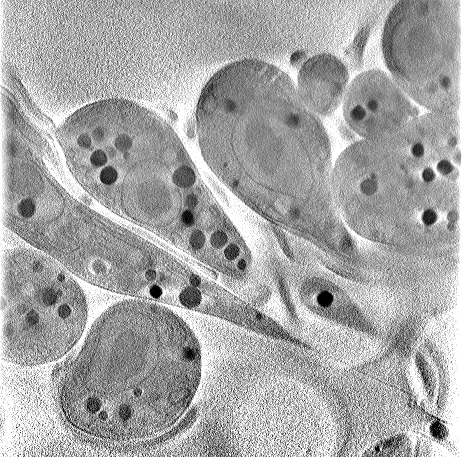
\includegraphics[width=0.27\textwidth]{Applications/thumnail.png}
\end{wrapfigure}

This chapter explores some behaviour of iterative algorithms implemented on GPUs and shows how some of the algorithms behave with different datasets. Firstly some numerical experiments are performed for digital phantoms, analysing the effect of angle ordering on SART-type algorithms, hyperparameter reduction methods and observing the behaviour of the different TV algorithms included in TIGRE. Then some real datasets are reconstructed using a variety of the algorithms presented in previous chapters, from medicine (a head phantom from the Christie Hospital), micro-tomography (the Sofia-beads dataset) and synchrotron tomography (some cryo soft X-ray tomograms). One of these last datasets is then segmented using the {SuRVoS} workbench to highlight the differences.


\FloatBarrier
\subsubsection{Chapter 6: motion compensation modelling}

\begin{wrapfigure}{l}{0.35\textwidth}
\centering
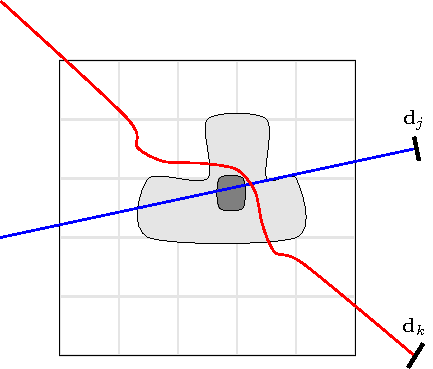
\includegraphics[width=0.32\textwidth]{MotionCorrection/diagrammotion1.pdf}
\end{wrapfigure}

Using the theory from phase space tomography at CERN, this chapters proposes a motion compensation algorithm for when the motion is approximately known. By modelling the X-rays as warped paths instead of straight lines on the GPU. The GPU implementation is described and two experiments are presented, one with synthetic data and deformation  vector fields, and another one using a 4D-CT dataset. Results show that when the motion is perfectly known the method performs equally well to a reconstruction without motion and that the method can give better information about the tumour using the same amount of projections as a CBCT image. As the method relies on modelling the motion in the basic building blocks of CT reconstruction, it can be used in any existing iterative algorithm.



\newpage
\FloatBarrier
\subsubsection{Chapter 7: Numerical Study of Motion Compensation}

\begin{wrapfigure}{L}{0.35\textwidth}
\centering
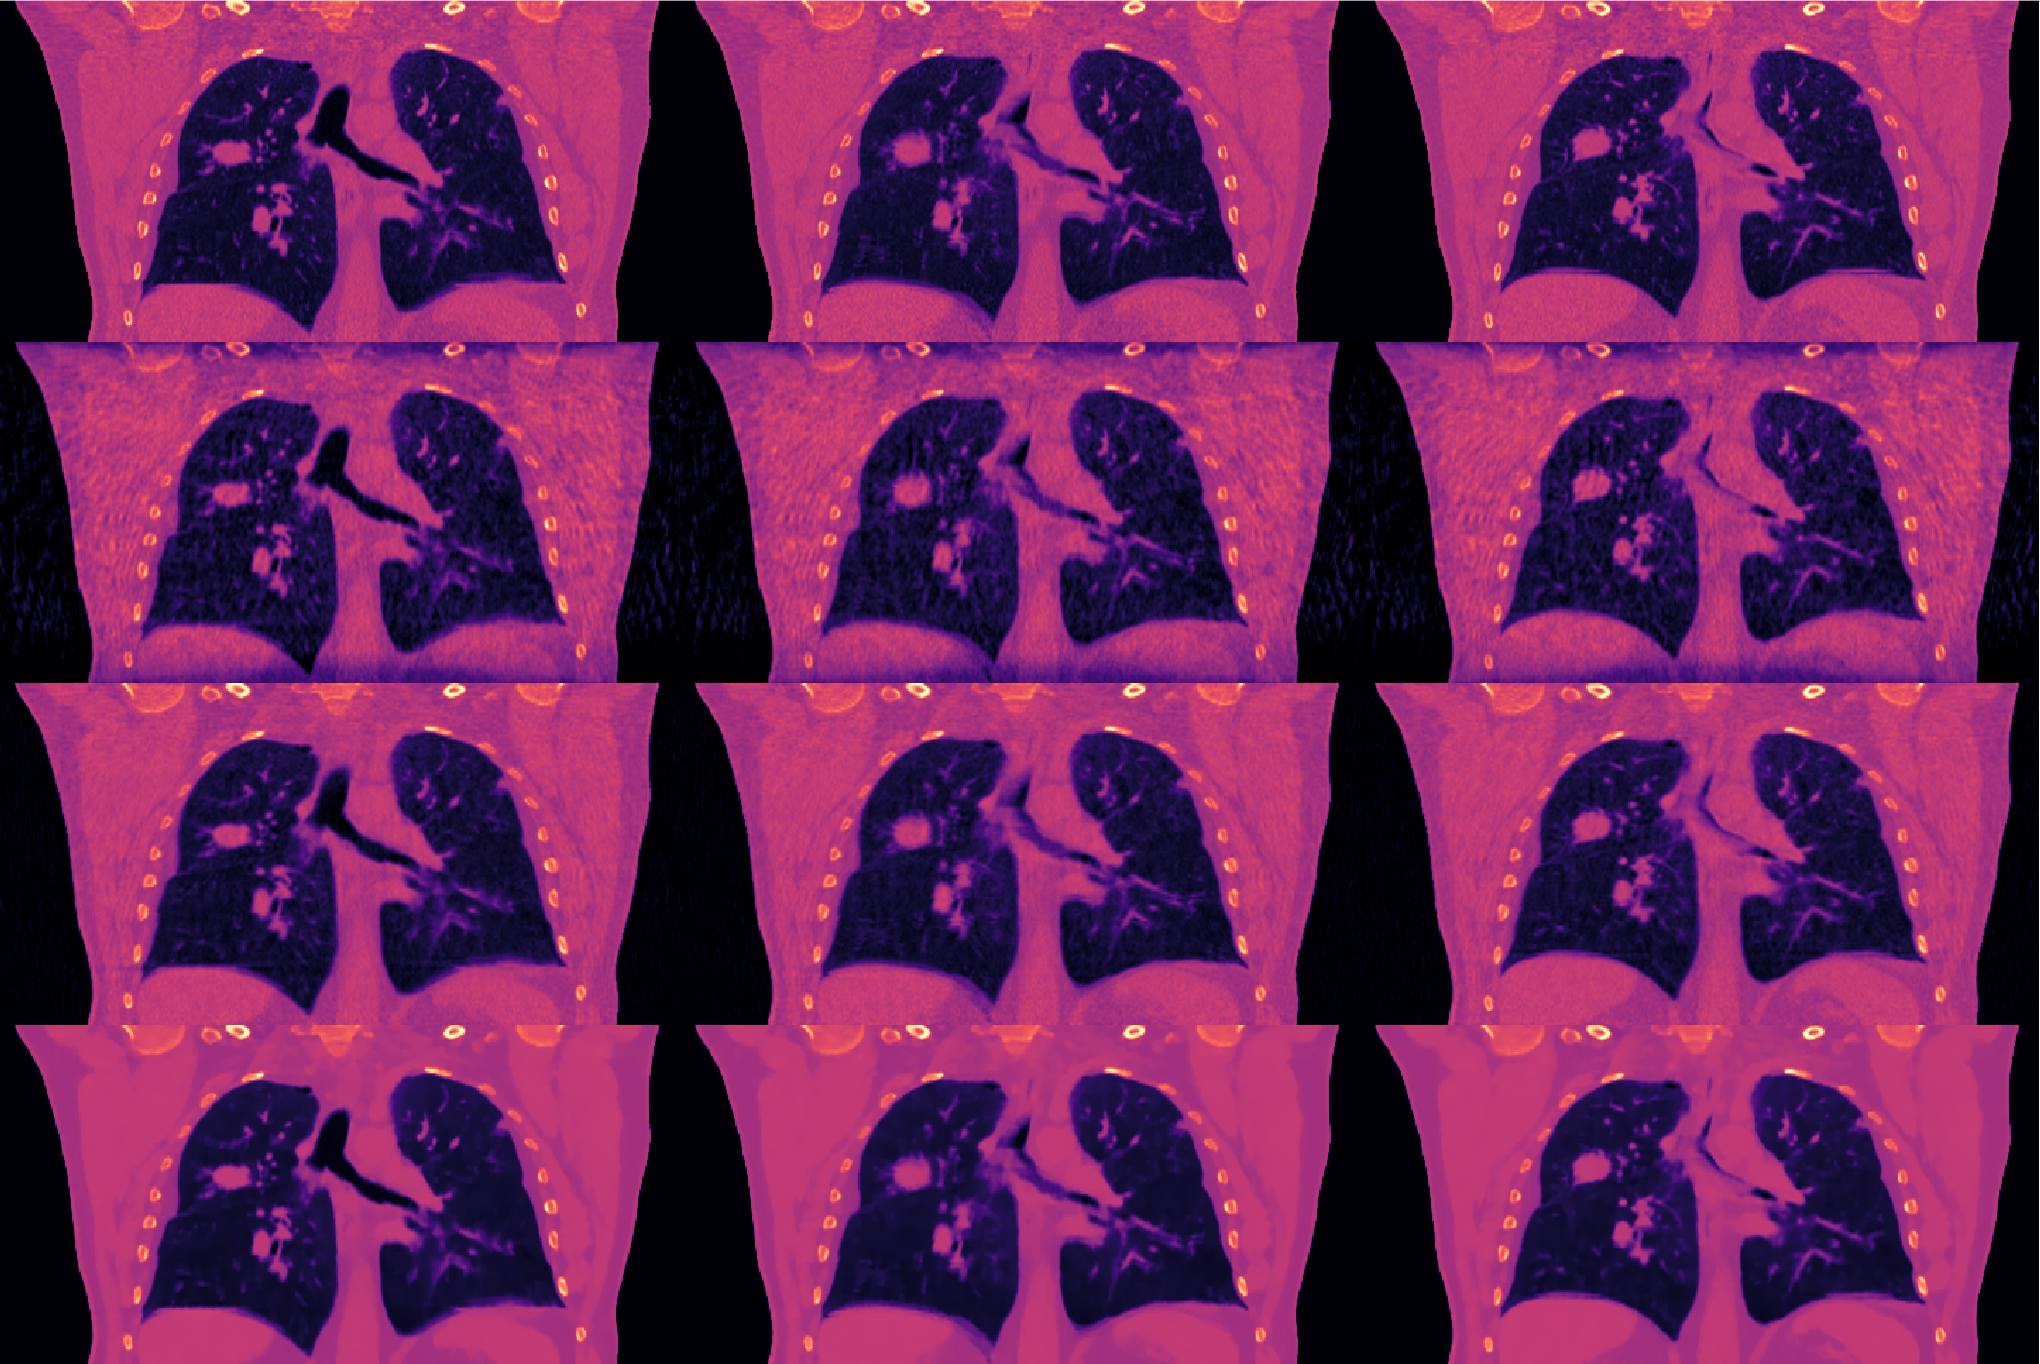
\includegraphics[width=0.32\textwidth]{accuracyMC/4DCBCT3stage.png}
\end{wrapfigure}
The previous chapter described a method for motion compensation. This chapter focuses on numerically testing the limits of the method, as obtaining perfect motion information is an almost impossible task in medical applications. The chapter shows that the performance of the method is very similar (with marginally bigger error) than 4D-CBCT, with an order of magnitude less projections, thus less radiation to the patient. Tests against the most common numerical errors in medical applications are performed: very low resolution motion information, errors in the binning process of projections (thus in the motion information) and the case where only the motion of the tumour is known. In all cases, the motion compensation method has errors of less than a voxel in tumour location, and very small mismatch in the volume selection of the tumour.




\FloatBarrier


\section{Publications and contributions}

The work on this thesis was been published either as open source software or publications in conferences and peer reviewed journals. The following publications directly relate to the content of this thesis:

\begin{itemize}
\item ``GPU based iterative CBCT for prospective motion compensated algorithm for radiation therapy''\cite{biguri2016gpu}. Short paper based on the presentation at the conference ICTR-PSE 2016. \tb{The author of this thesis contribution has been the writing up of the entire toolbox presented. The other authors supported this work with contribution on the context, importance and presentation of the work.}
\item ``TIGRE: A MATLAB-GPU toolbox for CBCT image reconstruction''\cite{TIGRE}. Journal article condensing the research in Chapter 3, Chapter 4 and Chapter 5. \tb{Similarly as the previous article, most of the article and code has been written by the author of this thesis. The other authors supported this work with contribution on the context, importance and presentation of the work.}
\item  ``A General Method for Motion Compensation in X-ray Computed Tomography''\cite{biguri2017general}. Journal article on Chapter 6. \tb{The original idea came from S. Hancock, A. Biguri translated that knowledge into a practical algorithm with GPUs for the medical case, due to the difference in scale an physics of the problems. M. Dosanjh contributed with the biomedical knowledge of the relevance of the methods for IGRT and M. Soleimani with supervision on the project and mathematics.}
\end{itemize}

This work has been also presented in various conferences and meetings, via posters or presentation talks. Posters have been presented at ToScA 2016 with the title ``TIGRE: Tomographic Iterative GPU-based Reconstruction toolbox''\cite{biguri_ander_2016_159016}, in the ENLIGHT 2016 meeting titled ``Motion correction in X-ray tomography using a priori known deformation vector fields and iterative reconstruction methods''\cite{biguri2016motion} and in BIGART 2017 titled ``Improvement of image quality in 4D-CBCT respiratory correlated and motion-compensated reconstruction using iterative algorithms and GPU acceleration''\cite{biguri2017motion}. The work has also been presented in various talks and seminars. Finally, a Medical Physics Web article by Tami Freeman is available for wider audiences at \href{http://medicalphysicsweb.org/cws/article/research/66343}{http://medicalphysicsweb.org/cws/article/research/66343}.

The TIGRE Toolbox and specifically some of the total variation based image recosntruction code has been also used in the article ``Parameter selection in limited data cone-beam CT reconstruction using edge-preserving total variation algorithms'' by Lohvithee \textit{et al}\cite{Vee}.

\subsubsection{Other publications}

During the course of the PhD, mainly in the early stages, other work was published focused on dual modality electrical impedance tomography (EIT) CBCT, as some initial work explored the use of EIT for real time tumour tracking. That work is not presented in this thesis, but has been published in a few items. The work is summarized in a peer reviewed journal article ``Tracking boundary movement and exterior shape modelling in lung EIT imaging''\cite{biguri2015tracking}, and extended in peer-reviewed conference articles for the EIT 2015 meeting in the works titled ``Statistical and deterministic approaches for electrode movement in lung EIT''\cite{biguri2015statistical} and ``4D FEM models of the human thorax''\cite{biguri20154d}. Initial work in this field was also presented as a poster in the ENLIGHT 2014 meeting titled ``Dual modality EIT-CBCT for lung radiation therapy''\cite{biguri2015dual} and in AIP 2015 as ``Electrode movement due to breathing in lung EIT imaging''\cite{biguri2015electrode}.






\chapter{Image guided radiation therapy and computed tomography}\label{ch:soa}

This chapter explores the relevant state of the art for the work in this thesis. First, a short introduction of the technique used in IGRT, especially in lung IGRT is presented, with a focus on the lung imaging. This shows how CBCT is a widely used technique in IGRT and how dealing with motion is key. Then a small introduction of other uses of CBCT is presented. Later, CERN's phase space tomography and its motion compensation method is described. The techniques used for removing motion in CERN's proton synchrotron is the basis for the methods presented in chapters 6 and 7. Finally, the relevant literature for dealing with motion in CBCT is presented.


\section{Image Guided Radiation Therapy}
Radiation therapy is a widely used cancer treatment, generally performed by radiating very high energy photons into the body to damage the cancerous cells. Nowadays hadrons (charged particles) can also be radiated to the malignant tissue, the benefit of these being that they mostly only damage the targeted area. For both, specially for hadron therapy, knowing the exact shape of the patient and the tumour is highly important to properly deliver the X-ray dose only (or mostly) to the malignant tissue and to spare as much healthy tissue as possible. Imaging the patient accurately is crucial and can potentially increase survival rates and lower morbitidy rates\cite{nguyen2015potential}.

There are two separate cases for imaging in radiation therapy: the planning stage and the treatment stage. Before any radiation surgery is performed, a high definition of the patient's body is needed, not only for the tumour, but also the rest of the tissues. This is because, in the planning stage of  the radiation delivery, knowing the exact amount of tissue (the electron density of the tissues more precisely) that each X-ray beam needs to cross helps planing the dose delivery steps and the overall expected tissue damage. This is generally done with high energy, high resolution CT scans. Nowadays other modalities are starting to be used, such as magnetic resonance imaging (MRI)\cite{schmidt2015radiotherapy} and positron emission tomography (PET). MRI has a high potential of replacing CT for planning, as there is no radiation to the patient and arbitrary oblique planes can be reconstructed, but MRI has multiple challenges to solve: high acquisition times, lack of electron density maps (generally solved by registering with a CT) or some geometric deformations that MRI has intrinsically. PET is not used instead of CT, but together with CT. PET images show functional information, by showing the location of some specific molecules that can be chosen. It is used to clearly delimit cancerous cells, and usually used together with CT\cite{soykut2013use} or MRI. By fusing PET images with structural image modalities, the delineation of the tumour can be done with higher accuracy. 

The second area where imaging is used is in the treatment stage. Patients change physiology during treatment, and the tumour itself changes shape and size as it's being treated. Additionally, knowing the real dose being delivered and comparing it to the planned dose is important. One of the most common treatment imaging systems is CBCT\cite{ding2007study}, due to its ability of generating 3D images with low dose compared to comventional CT. MRI can be used for both dosimetry\cite{ozenne2017improved} and on site (even live) imaging. This last one, the MRI-linac, has great potential for improving photon IGRT, as it can get real-time images of the patient during the treatment process\cite{LAGENDIJK200825}. However, the use of MRI for real time imaging in hadron therapy is a bigger issue, as the strong magnetic forces (generally about 1.5T) would modify the path of the radiation beam because hadrons are charged particles. While MRI linac may replace the widely used CBCT in conventional radiation therapy, CBCT still has a very strong role in current and future RT.

CBCT however has two main problems that need to be tackled to improve IGRT. The first is that CBCT does not reconstruct Housnfield Units with the same accuracy as conventional CT, thus the electron density is not correctly known. This is a key factor for correct treatment dose planning. Generally this issue is solved as with MRI, by registering the image to a prior CT or a CT atlas. The second and more harming problem is motion. Due to the lower doses used than in a conventional CT scan and to its slow data acquisition rate, a CBCT image is generally riddled with noise and motion artefacts. This is a major problem for tumours such as lung and liver, as these move with the breathing of the patient, and much research is being carried out to solve this issue.


\section{CBCT imaging in other applications}

While CBCT is widely used in IGRT, its use is more widespread in both the medical and other applications. In medical applications CBCT is widely used in dental applications\cite{alamri2012applications}, as it has the ideal contrast for the bone structure of the head, thus being a good minimally invasive technique for dental imaging. CBCT is also used for guidance in surgery, generally known as interventional radiology, in applications such as renal and prostate embolization\cite{floridi2014c}, stent placement, sclerotherapy, thoracentesis\cite{Acord2017}, among others. It is specially used in paediatric surgery, as it minimizes the X-ray dose to young patients comparing to other CT modalities.

Outside medicine, the CBCT geometry is widely used in micro-tomography, named after the size of the pixels, that can get to micrometer sizes. Due to the small size of the samples, the cone beam shape is the only possible shape that can practically fit in a machine in a standard laboratory, without using a synchrotron (electron accelerators that generate high quality X-rays). Its applications in research are wide, from archaeology, biology, material science, crop studies, geology, space, and many more.

Finally, CBCT applications are starting to get used in industrial applications, very often on the micro-scale that research applications use, but also for larger resolutions. The main applications in industry, apart from the industrial research purposes, is quality control and metrology. Often non-destructive quality control of complex pieces can only be performed with X-rays. Similarly, often manufacturing processes of complex pieces have the problem that is hard to measure the exact sizes produced, but CT is able to reconstruct and then measure distances accurately.
% SOME IMAGES? 
\section{Phase Space Tomography at the proton Synchrotron}

Motion in tomography is a problem not only in X-ray modalities. Phase space tomography is a hybrid algorithm that combines particle tracking in a computer model of a synchrotron with iterative algorithms to reconstruct an image of the population of a bunch of particles circulating in the accelerator. The particle motion involves non-linear rotation and is non-cyclic, but a 1D projection of the distribution can be completely acquired as a single snapshot on one turn of the machine. By tracking test particles to gain a knowledge of how the geometry of the 2D image plane (longitudinal phase space) deforms, the information in all the discrete time slices acquired over many turns can be translated back to the same instant and topographically combined in a single image. This is possible because the motion of the particles can be precisely known from understanding and measuring the physics in their acceleration. To do so, each pixel in the reconstructed image is populated with a bunch (generally 16) phantom particles, and their movement is simulated. By knowing in which measurement bin each fraction of the pixels (each phantom particle) falls in each position in time, the tomographic reconstruction can be performed by assigning values to the locations of these particles in the desired time position. Figure \ref{fig:PST} shows the measured projections and reconstructed images using these technique. If the motion modelling were not included, the swirl pattern would not be visible.

\begin{figure}

\begin{center} 

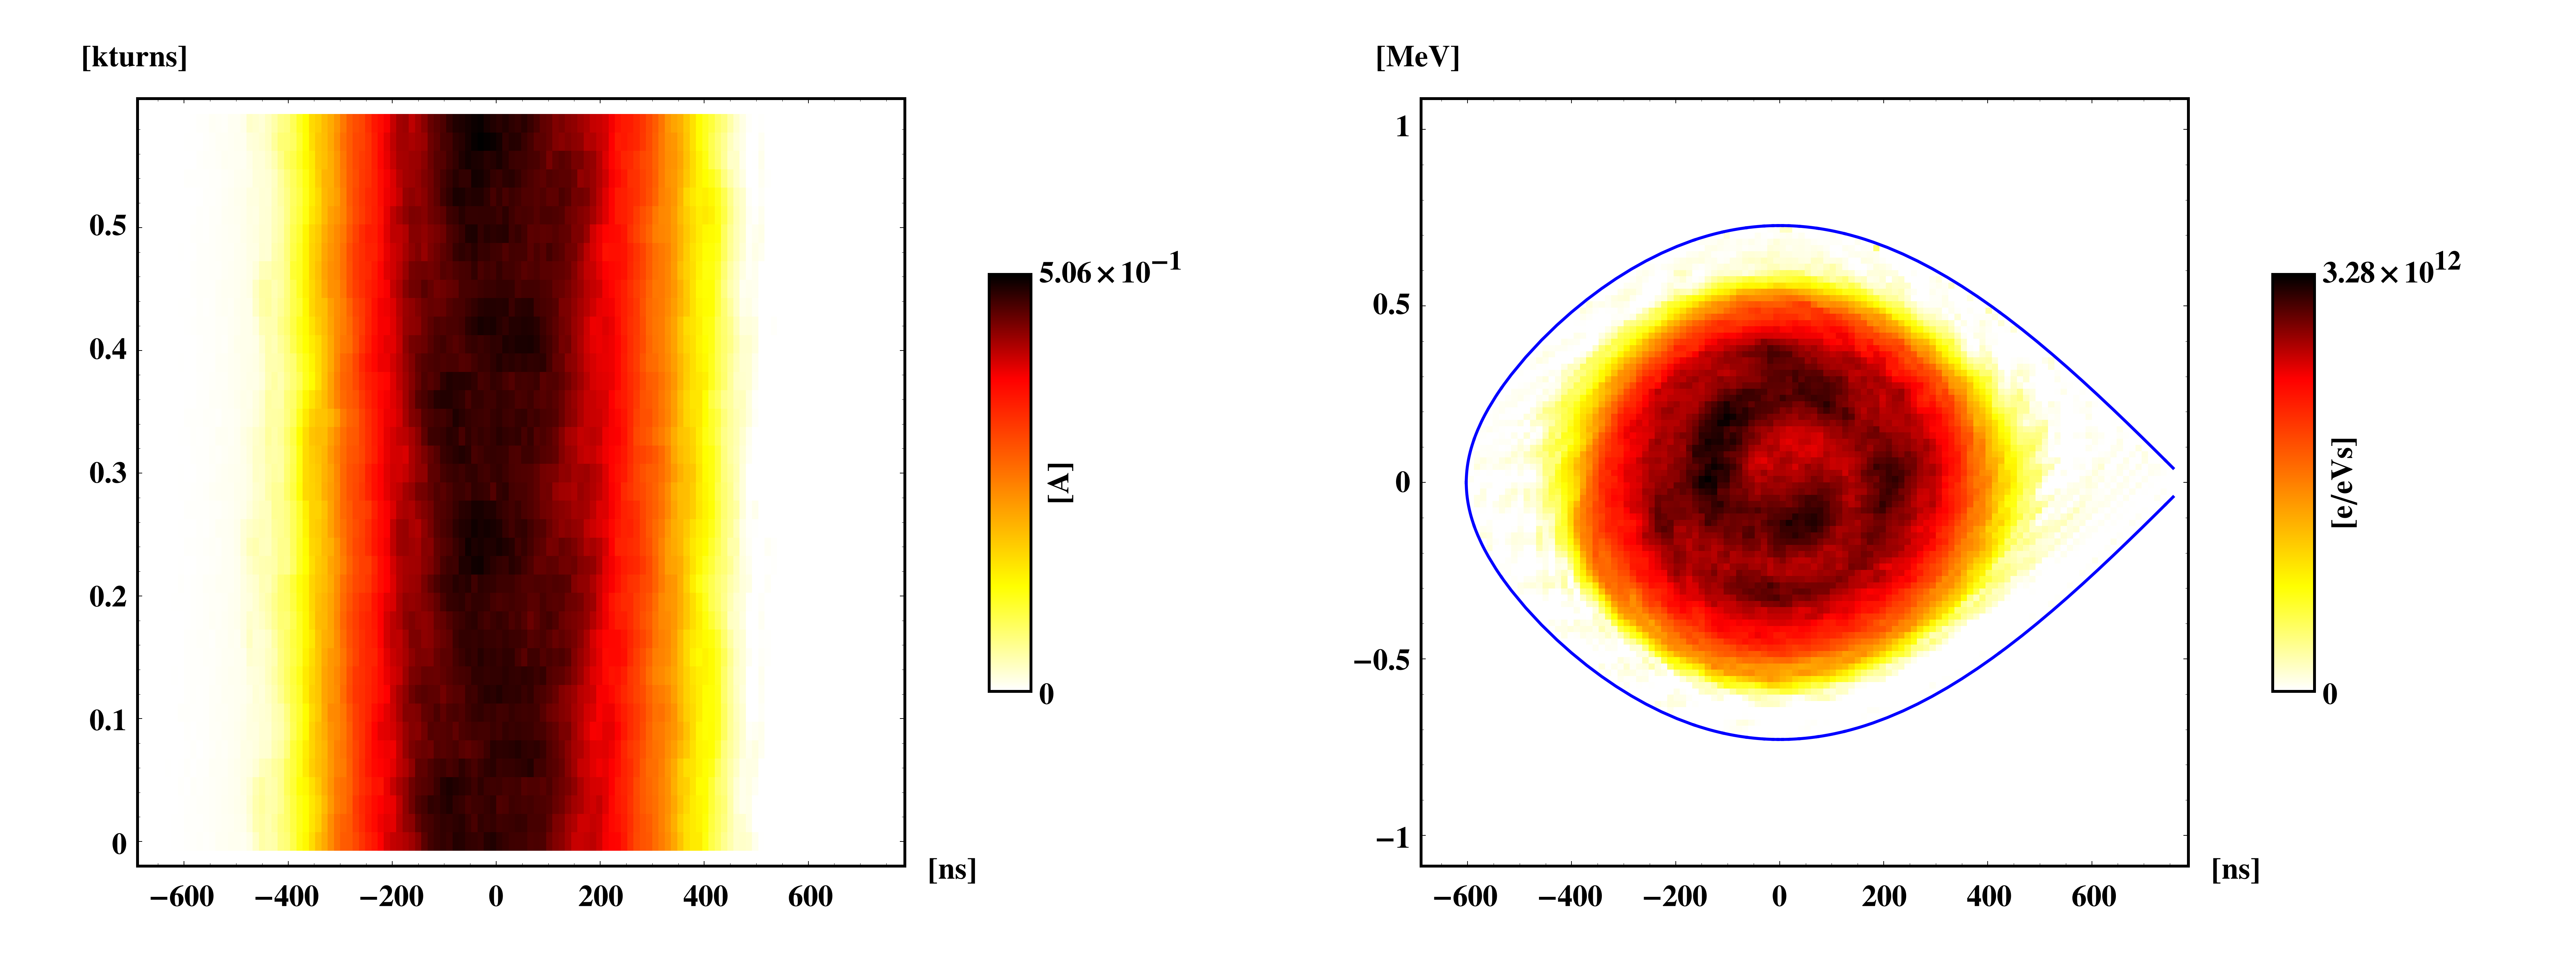
\includegraphics[width=\linewidth]{StateOfArt/Tosca2016fig.png} 

\caption[Phase space tomography]{\label{fig:PST} Early example (1999) of a set of 1D bunch profile data (left) processed into a 2D image of particle density in the longitudinal plane (right) using phase space tomography.  The resultant particle distribution is consistent with all the measured profiles and the physics of synchrotron motion.  The detailed internal bunch structure that is revealed is a consequence of the non-linearity of the motion.  The measurement was made at the CERN Proton Synchrotron Booster.\cite{pstweb}.} 
\end{center} 
\end{figure}


 Conceptually the method means adding the motion information to the geometry of the model with which the problem is posed rather than inserting it somehow into the mathematics of the tomography by which a solution is found. However, the specific technique used in phase space tomography is not viable in medical imaging, as the images are already very big in pixels, increasing the size e.g. 16 times would be computationally infeasible. Thus, the concept of phase space tomography must be implemented using a different method in CBCT.

\section{Motion in CBCT}
 Research into the removal of motion artefacts in CBCT is widespread and numerous articles have been published on the subject.  The most studied method to deal with motion is phase-correlated CBCT, also called 4D-CBCT\cite{sonke2005respiratory}\cite{thomas2006}\cite{li2006four}\cite{Pengpan2012246}\cite{t2016first}.  In 4D-CBCT, projection data are binned according to respiratory phase and then the data from each bin are reconstructed separately to produce a series of images.  This approach has several drawbacks.  Even though the amount of data per reconstructed image is smaller than usual, the total number of projections increases which means a longer irradiation time and a higher dose for the patient, limiting its clinical use.  In addition, the image quality of each 4D-CBCT reconstruction is inferior to a 3D-CBCT one due to its reduced angular sampling and to small inconsistencies resulting from binning inaccuracies. 

Due to the limitations of standard 4D-CBCT imaging, extensive research has been conducted to improve the quality of the images.  This work can be divided into two main groups: algorithmic approaches and deformation vector field (DVF) optimization methods.  Methods in the first group rely on regularization and other similar approaches.  An example is the work by Jia \textit{et al.}\cite{jia2012}, who implemented a non-local means of reconstruction to improve the temporal similarity between images.  Total variation methods (TV)\cite{ASD_POCS}, which minimize gradients within an image, have also been proposed with a temporal dimension included in the gradient\cite{0031-9155-57-6-1517}.  Another method based on TV minimization is the so-called PICCS algorithm\cite{chen2008prior}\cite{0031-9155-53-20-006}\cite{chen2012time} (it is actually a regularizer), which minimizes the TV and the difference between the reconstructed image and a prior image.  This prior image is generally a CBCT reconstructed with motion artefacts.  PICCS can reconstruct 4D-CBCT images from highly undersampled datasets.  More complex algorithms have also been proposed, such as ROOSTER\cite{:/content/aapm/journal/medphys/41/2/10.1118/1.4860215}, where a series of regularizations and minimizations are performed inside a region of interest to create clear 4D images in that area.

The methods of the second group generally (but not always) rely on a previous high-quality 4D-CT treatment planning scan as the basis from which to compute the DVFs.  As breathing motion is neither truly periodic nor reproducible in a given patient over time, the DVFs are corrected by matching real projections with simulated ones.  Finally, when the best DVF is computed, a synthetic image is generated by deforming the prior high-quality CT scan.  Examples include the work of Brock \textit{et al.}\cite{brock2010} and Ren \textit{et al.}\cite{Ren20121584}, who managed to reduce the number of projections required to about 60 using non-linear conjugate-gradient methods.  In order to improve robustness and reduce the dimensionality of the problem, DVF principal component analysis methods have also been proposed\cite{zhang2010correction}.  Li \textit{et al.}\cite{:/content/aapm/journal/medphys/37/6/10.1118/1.3426002}\cite{:/content/aapm/journal/medphys/38/5/10.1118/1.3582693} demonstrated that good accuracy can be achieved using only a single projection for the DVF optimization.

Hybrids between DVF-based and algorithmic approaches also exist, such as using TV regularization methods to improve convergence by initializing the DVFs\cite{wang2012high} or using temporal regularization with DVFs to improve the ROOSTER algorithm\cite{mory2016motion}.  Hybrid methods can lead to highly complex optimization strategies.  Examples include segmented mesh-based 4D-CBCT\cite{0031-9155-61-3-996} and the separation of static and moving images using TV, tight frame regularization and DVF optimization\cite{0031-9155-56-11-002}.  In addition, Christoffersen \textit{et al.}\cite{christoffersen2013registration} have proposed a multi-step algorithm using TV and optical flow for motion estimation.

Finally, some special mathematical algorithms have also been suggested that are unique in their approach.  These include the cine-CBCT algorithm\cite{6803058} and the 5D motion modelling approach\cite{0266-5611-31-11-115007}, which does not use phase-correlated binning.

The literature is full of these and many other approaches, ranging from the computationally and mathematically complex to those that sacrifice accuracy for simplicity and speed.  Most have been shown to yield good 4D-CBCT reconstructions, some in clinical scenarios.  But they all have drawbacks.  CBCT is a severely ill-posed problem where the amount of data is key for a good reconstruction.  The simplest methods that rely on binning will always suffer to some extent from a lack of data, even if temporal coherence is enforced with mathematical norms.  Additionally, they involve the reconstruction of several images, which is very expensive both computationally and in terms of memory.

Most DVF-based approaches ultimately use the DVFs to deform a prior image rather than using the acquired data directly to produce a reconstruction.  Further, they assume that a DVF can describe every possible anatomical change with respect to that prior image and this does not necessarily hold.

%{red}{\sout{Here, we propose a completely different approach to motion compensation in 4D-CT imaging.}}
In this work, a modelling method for motion compensation is presented, as first proposed by Hancock \textit{et al.}\cite{pst1} outside the medical domain and later independently proposed by Rit \textit{et al.}\cite{Rit1}\cite{Rit2} for CBCT. Since the publication of their work, computing on graphical processing units (GPUs) has taken a significant leap forward affording more modern techniques that can be used to reconstruct with greater accuracy and computational efficiency. With the use of GPUs even generic motion compensation is possible, without any numerical approximation of the weights in the projection and back projection and using better forward modelling\cite{fwdproj}. Such an approach is presented in this work.

This thesis focuses on thorax CBCT, but the method is generalizable to any X-ray absorption CT modality and to arbitrary motion.  The method requires no binning, but instead uses all projections to reconstruct an image at any respiratory phase.  It does require a sufficiently accurate description of the motion in terms of DVFs, but the approach is a modelling one so it can be used to introduce motion compensation into any iterative reconstruction algorithm. 

\section{Discussion}

Hopefully the topics presented in this chapter clarify why motion is a key problem to solve in IGRT and hadron therapy and why the solution should start by being able to image in 4D. The concepts in phase space tomography can not only  potentially solve the problem, but can do so by reducing the amount of data acquired significantly. This concept has barely been explored in the literature. Additionally, any general improvement on image quality in CBCT would not only benefit medical applications, but a entire set of different uses of the imaging technology.
\chapter{The image reconstruction problem}

%Reconstructing accurately the desired domain is a complicated mathematical problem that is actively being researched since the invention of CT. However, nowadays the FDK algorithm is the most widely used algorithm, and only until very recently [CITE] it has been the only algorithm available in any commercial medical reconstruction device. While using FDK is advantageous in some cases, often the algorithm behaves poorly, specially when errors arise in the data, or the amount of data is limited. This is because FDK is based on a derivation of straight path integrals in continuous spaces. Reality is far from straight path integrals, as due to X-ray physics photons do not behave linearly. Photons from CT machines are polychromatic, and human tissue is behaves non-linearly in respect to X-ray energy. Additionally, Compton scattering is a common effect, where the photons get reflected in different angles dependent on their energy. Apart from physics, electronic noise is always present in detector technology being the only feasible way of avoiding it longer exposition times, harmful to live tissue. Limited data can additionally harm the image reconstruction, as CT has generally less detector data than the amount of  voxels are desired to reconstruct. All these effects make CT image reconstruction a challenging problem and have strong effect in the behaviour of FDK. As an alternative to FDK, iterative algebraic reconstruction algorithms try to minimize the error by updating the image continuously and comparing it to the measured data. These algorithms have been shown to improve reconstruction quality when the data is noisy and/or limited. Additionally, as they are an algebraic tool, they allow careful tuning of the mathematics on there, enabling them to be tuned to correct any chose effect. 

This chapter tries to explain the mathematics behind CT reconstruction, the FDK algorithm and iterative reconstruction algorithms. After the formal proposition of the mathematical problem of integrating over straight lines,the FDK algorithm is introduced. Then, the alternative proposal of the iterative algebraic methods is shown, followed by a wide variety of different algorithms that can be used to solve the algebraic problem. These include gradient descend techniques, Krylov subspace methods, statistical approaches and compressed sensing techniques. Finally, a discussion of the challenges that arise from the use iterative algorithms are described.  

\section{Geometry of CBCT}

\section{FDK}

\section{Iterative reconstruction algorithms}
Nowadays the FDK algorithm is the most widely used algorithm, and only until very recently [CITE] it has been the only algorithm available in any commercial medical or industrial CT device. While using FDK is advantageous in some cases, often the algorithm behaves poorly, specially when errors arise in the data, or the amount of data is limited. This is because FDK is based on an analytical approximation of straight path integrals in continuous spaces. Reality is far from straight path integrals, as due to X-ray physics photons do not behave linearly. Photons from CT machines are polychromatic, and human tissue is behaves non-linearly in respect to X-ray energy. Additionally, Compton scattering is a common effect, where the photons get reflected in different angles dependent on their energy. Apart from photon physics related errors, electronic noise is always present in detector technology being the only feasible way of avoiding it longer exposition times, harmful to live tissue. Limited data can additionally harm the image reconstruction, as CT has generally less detector data than the amount of  voxels are desired to reconstruct. All these effects make CT image reconstruction a challenging problem and have strong effect in the behaviour of FDK. As an alternative to FDK, iterative algebraic reconstruction algorithms try to minimize a functional by updating the image continuously and comparing it to the measured data. These algorithms have been shown to improve reconstruction quality when the data is noisy and/or limited. Additionally, as they are an algebraic tool, they allow careful tuning of the mathematics, enabling them to change their behaviour.

Iterative algorithms in CT generally reffer to those algorithms that, as the name says, iterate, but solve the linearized model 
\begin{equation}
Ax=b+\tilde{e} \label{eq:linearized model}
\end{equation}
on where $x\in \mathbb{R}^{N_{voxels}}$ is a vector representing the lexicographically ordered voxels of the 3D image, $b\in \mathbb{R}^{N_{pixels}} $ a vector of the detector measured pixels. $A$ is the linearized model matrix, a matrix that describes the behaviour of the CT system. Each row of the matrix $A$ is describes the behaviour of the X-rays that affect each single pixel in the detector. However, this matrix is so big that in practize its explicit form is impossible to store, and the matrix product operations $Ax$ (or projection) and $A^Tb$ are implemented instead. The next chapter goes into a bit more detail on how to operate with matrix $A$ and its limitations. Errors from measurement are inevitable in any application, and there are linearization errors, as no model is perfect. In equation \ref{eq:linearized model}, $\tilde{e}$ represents all those errors.

As an exact solution for $x$ can not be found, the problem in equation \ref{eq:linearized model} is minimized as
\begin{equation}
\hat{x}=\argmin_x \lVert Ax-b\rVert^2+R(x),\label{eq:THE equation}
\end{equation}
on where $R(x)$ is an optional regularization function. This minimization function has been widely studied in mathematics and there are multiple algorithms that can solve it. However not all algorithms that solve the equation can be used in CT reconstruction, due to the nature of the $A$ matrix, as it is very big (approximately $10^8\times 10^8$ in a standard medical image) and very sparse (approximately $0.0017\%$ of sparsity in a standard medical image). This makes the matrix severely ill-conditioned and impossible to store in memory. Additionally, often the CT problem can be underdetermined, making the problem ill-posed and further constraining the possible algorithms that can be used. That said, a wide variety of algorithm have been proposed to solve the CT algebraic problem and new ones are still being published. This section discusses a few of the available and most common algorithms that have been studied in this work.


\subsection{Algebraic Reconstruction Techniques}

Arguably the most well known iterative algorithm is the method known as the algebraic reconstruction technique (ART)\cite{K-1937}, known as the Kaczmarz method outside the CT imaging field. The ART algorithm, for matrix elements $a_{ij}\in R$ is defined as
\begin{equation}
x^{n+1}=x^n+\frac{b_i-\langle a_i,x^n\rangle}{\lVert{a_i}\rVert^2}a_i^T,
\end{equation}
where $a_i$ is the $i$-th row of matrix $A$ and $\langle \,, \rangle$ denotes the inner product. The ART method projects the image into the hyperplane described by the equation in row $i$. Generally the method includes a relaxation parameter $\lambda_n$ that controls the update size, and that decreases with the iteration number. This generally avoids the cyclical convergence that the method describes when the solution is not unique (the intersection of the hyperplanes is not a single point). By relaxing the update step, the algorithm converges to a single point. Generally the algorithm is also run with some inequality constrains, the most common one being a positivity constrain for $x$, as negative values are not physically possible.

Studies on the convergence of the ART algorithm show\cite{241889} that randomly choosing the order of the rows in each iteration ($n$) increase the convergence rate, even more if the probabilities of picking rows are different than one (different methods propose different probabilities)\cite{strohmer2009randomized}\cite{liu2016accelerated}. 

However, the ART method has a major disadvantage: the image $x^{n+1}$ needs to be updated $i$ times each iteration. In current CT applications, and specifically in CBCT, the amount of rows in the matrix i.e. the total amount of independent pixel measurements in the detector is a massive number. Following the same definition of standard medical image size from the thesis, a $512\times512$ detector, with 360 projection means that the amount of rows is in the order of $10^8$. In order to update the image less, the Simultaneous Iterative Reconstruction Technique (SIRT)\cite{SIRT} can be used, a method that is very similar to Cimmino's method, that updates the image using simultaneously (instead of sequentially) all data in the measurement $b$, thus each iteration is a single update. While SIRT generally solves the problem of the high amount of updates in ART, it suffers from a very slow convergence in comparison, and will generally plateau in a solution that is not as good as what ART provides. The SIRT algorithm can be described in matrix form as
\begin{equation}
x^{n+1}=x^n+\lambda_n V A^T W^{-1}\left(b-Ax\right) \label{eq:SIRT}
\end{equation}
where $V=1/\text{diag}\bigl({\sum_j a_{ij}}\bigr)$ and  $W=\text{diag}\bigl({\sum_i a_{ij}}\bigr)$.

However, middle ground has also been proposed. Kak and Andersen proposed\cite{SART} the Simultaneous Algebraic Reconstruction Technique (SART) on where the image is updated using simultaneously all data from each X-ray projection, but still updating the image multiple times per iteration. Finally, the update can also be done using block-based methods, or Oriented Subsets (OS) with a variety of methods generally described as OS-SART\cite{OS_SART} methods.

 Similarly as with ART, the order of the subsets in both OS-SART and SART have influence in the convergence, with a lower impact than in ART. In this work an three methods have been implemented, a completely ordered method, a randomized ordered method with full sampling (i.e. all projections are ensured to be used once and only once per iteration) and an angular distance based one. This last one orders the subsets by selecting the next one as the subset with largest angular distance from the ones already used. The heuristic rationale is that the projections at larger angular distance update the image by a bigger step than projections angularly near. In all further result in this thesis, the default ordering is random, unless otherwise explicitly stated.
 
 %% SHOW CONVERGENCE WITH DIFFERENT ORDERING



\subsubsection{Relaxation parameter $\lambda$}

As previously mentioned, changing the relaxation parameter per iteration can be of advantage, by avoiding cyclical convergence and often by increasing the general convergence rate. On of the commonly used methods for the reduction of lambda is simply reducing it by a reduction factor each iteration as
\begin{equation}
\lambda_{n+1}=\lambda_n*r_\lambda
\end{equation}
where $r_\lambda$ is some value close to one, such as $r_\lambda=0.99$ or $r_\lambda=0.999$. However this method, while useful to avoid cyclical convergence in ART methods, is of less use in simultaneous methods, as it generally slows the convergence rate.% Alternatively, convergence studies for SART/OS-SART/SIRT algorithms have shown\cite{jiang2003convergence} that an update of the relaxation parameter in the form of
%\begin{equation}
%\lambda_{n+1}=\frac{\lambda_0}{1+n^\alpha}
%\end{equation}
%where $\lambda_0$ is an initial value of the relaxation parameter (usually 1) and $0<%\alpha\leq 1$. this can improve the convergence of the algorithms. 

It is worth noticing that this family of algorithms is very closely related to the well known gradient descend methods, as the gradient of equation \ref{eq:THE equation} is  proportional to $A^T(Ax-b)$, or in other words $V=I$ and $W=I$ in equation \ref{eq:SIRT}. The gradient descend methods have been widely studied in the past years\cite{sutskever2013importance}\cite{DBLP:journals/corr/Ruder16}, as the Neural Networks community tries to find faster converging methods to train the nets they research. Among other methods proposed, Nesterov proposed an accelerated version of the gradient descend\cite{nesterov1983method}, that obtains a rate of convergence of $1/n^2$. The proposed update   updates the result image in each iteration by pushing it in the current update and previous update direction combined. Nesterovs Accelerated Gradient (NAG) defines
\begin{align}
\lambda_{n+1}&=\frac{1+\sqrt{1+4\lambda_{n}^2}}{2}\\
\gamma_n&=\frac{1-\lambda_n}{\lambda_{n+1}}\\
y^{n+1}&=x^{n}-\frac{1}{\beta}\nabla f(x^n)\label{eq:Nesterov update 1}\\ 
x^{n+1}&=(1-\gamma_n)y^{n+1}+\gamma y^n
\end{align}
with $\lambda_0=1$ and $\beta$ being the Lipschitz smoothness of the function $f$. The line in equation \ref{eq:Nesterov update 1} can be replaced by the SART/OS-SART/SIRT update on equation \ref{eq:SIRT} to obtain an accelerated convergence rate. Some experimental results on the convergence of the algorithms can be found in Chapter 5.
\subsection{Conjugate Gradient Least Squares}

The conjugate gradient for the least squares problems (CGLS) 
\subsection{Statistical inversion}
\subsection{Total variation minimization with POCS}

Sometimes solving a regularized problem may result in a better final image than just trying to solve the data constrain with the model. This is especially useful in more ill-conditioned problems, such as when the data is very noisy (thus the model does not fit the data with accuracy) or when few projections are available (the system is more under-determined). In these cases, regularisation can add a user constrain in the image domain that pushes the algorithm towards an specific solution among all the multiple possibilities. While a variety of regularization techniques and norms exist, the most suitable for CT imaging is the total variation (TV) norm.

The total variation norm is defined as the sum of the 2-norms of the directional gradients of the variable,

\begin{equation}
\lVert x \rVert_\text{TV}=\sum_n\left\lVert \sum_\alpha\partial_\alpha x_n \right\rVert_2.
\end{equation}

Applied to CT imaging, the total variation norm is the sum of the total change occurred in the image. An image with less total variation would be an image that would have less change, or more flat, same valued regions. Regularizing with the TV norm as a minimization term will yield an image that is piecewise smooth and it happens that most of the objects imaged in CT scanners are piecewise smooth in linear attenuation, even more in medical CT imaging. 

However, solving the minimization problem in equation XX is not trivial with the TV regularization. One of the first robust algorithm is the so called Adaptive Steepest Descend, Projection Onto Convex Subsets, or ASD-POCS algorithm\cite{ASD_POCS}. This algorithm not only minimizes the data constrain with TV regularization but also adaptively controls the TV minimization update, in order to adapt its strength according to the data constrain update. Several adaptations and improvements of this algorithm have been proposed in the literature[CITES], all based in the same mathematical basis.  


\subsubsection{ASD-POCS}

The previous algorithms discussed in this chapter where unconstrained minimization methods. While the TV minimization problem can be solved similarly (see section \ref{sec:SART-TV}) formalizing the algorithm as a non-linear constrained minimization adds an advantage in the case where there system is under-determined. In an unconstrained problem such as in equation XX, the balance between the data constrain and the regularization constrain can be tuned via a hyperparameter, but in the case of an under-determined system, multiple solutions for the data fidelity term may exist. By reformulating it as it is shown in the rest of this section, the image with the same data fidelity 2-norm but the lowest TV norm can be chosen.

The minimization will yield an image $\vec{x}^*$ that minimizes 

\begin{equation}
\vec{x}^*= \argmin_x \lVert \vec{x} \rVert_\text{TV}
\end{equation}
subject to 
\begin{align}
\lVert A\cdot \vec{x}-\vec{b}\rVert &\leq \epsilon,\label{eq:nl-datafid}\\
\vec{x}&\geq 0.
\end{align}

As previously described in this chapter, the data fidelity on equation \ref{eq:nl-datafid} while desired to be zero, it will never reach to zero, due to inconsistencies in the data, model, noise, etcetera. Thus, in this algorithm it is introduced as a inequality constrain, instead of as the minimization problem itself. This introduces the parameter $\epsilon$ in the algorithm, the maximum 2-norm allowed for the data inconsistency. The problem in hand is now non-linear, due to the constrains, but convex.

The conditions for a constrained minimization to find the optimal solution can be obtained by satisfying the Karush Kuhn-Tucker conditions (a generalization of the Lagrange multiplies for inequality constrains). First, the Lagrangian for the current problems needs to be defined, as

\begin{equation}
\textbf{L}=\lVert \vec{x} \rVert_\text{TV}+\lambda_0\cdot(\lVert A\cdot \vec{x}-\vec{b}\rVert^2 - \epsilon^2)-\vec{\lambda}\cdot\vec{x},\label{eq:Lagrangian}
\end{equation}
where $\vec{\lambda}$ is a vector of the same size as the image, but $\lambda_0$ is a single value. Two inequality constrains are imposed to the Lagrange multipliers, namely non-negativity
\begin{equation}
\lambda_i \geq 0,
\end{equation}
and complementarity 
\begin{equation}
h_i(\vec{x}) \lambda_i = 0,
\end{equation}
where $i=0,1,..., N_{pixels}$, and $h_i$ is an alternative form of the inequality constrains as
\begin{align}
h_0(\vec{x}) &=\lVert A\cdot \vec{x}-\vec{b}\rVert^2 - \epsilon^2 \leq 0&\\
h_i(\vec{x}) &= -x_i \leq 0 & i \in [1, N_{pixels}]
\end{align}

Thus, only when the inequalities are violated does $h_i$ turns non-zero, and with the complementarity condition, does the corresponding $\lambda_i$ turns zero. A solution can be found for $\vec{x}$ when the gradient of the Lagrangian is zero, and if the differential operator is defined as

\begin{equation}
\nabla_{\vec{x}}Q(\vec{x})=\sum_i {\partial_{x_i}}Q(\vec{x}) \vec{\delta}_i
\end{equation}
where $\vec{\delta}_i$ is the Kronecker delta. The gradient of the Lagrangian can be then written as
\begin{align}
\nabla_{\vec{x}}\textbf{L}&=\nabla_{\vec{x}}\lVert \vec{x} \rVert_\text{TV}+\lambda_0\nabla_{\vec{x}}h_0(\vec{x})+\sum_{i=1\textit{•}}^{N_{pixels}}\lambda_i\nabla_{\vec{x}}h_i(\vec{x})=0 \notag \\
&=\nabla_{\vec{x}}\lVert \vec{x} \rVert_\text{TV}+2\lambda_0 A^T\cdot(A\cdot\vec{x}-\vec{b})-\vec{\lambda}=0 \label{eq:KKT}
\end{align}

Further simplification can be applied to equation \ref{eq:KKT}. As the non-negativity constrains are only active in zero valued voxels, the Lagrange multipliers are zero for strictly positive voxels. Thus, by adding an indicator function
\begin{equation}
\vec{x}_{indic}=
\begin{cases}
1 & \vec{x} \neq 0 \\
0 & \vec{x} = 0 
\end{cases}
\end{equation}
the Lagrangian gradient can be shortened to
\begin{equation}
\nabla_{\vec{x}}\textbf{L}=\text{diag}(\vec{x}_{indic})\left(\nabla_{\vec{x}}\lVert \vec{x} \rVert_\text{TV}+\lambda_0\nabla_{\vec{x}}h_0(\vec{x})\right)=0 .\label{eq:KKT2}
\end{equation}
Separating this new equation into two vectors,
\begin{align}
\vec{d}_{\text{TV}}&=\text{diag}(\vec{x}_{indic})\left(\nabla_{\vec{x}}\lVert \vec{x} \rVert_\text{TV}\right)\notag\\ 
\vec{d}_{\text{data}}&=\text{diag}(\vec{x}_{indic})\left(\nabla_{\vec{x}}h_0(\vec{x})\right)
\label{eq:KKTvectors}
\end{align}
brings to the Karush Kuhn-Tucker conditions: $\vec{x}$ will be an optimal condition if $\vec{d}_{\text{TV}}$ and $\vec{d}_{\text{data}}$ are pointing in exactly the opposite direction. In practice the algorithm will only check if the vectors are pulling in opposite direction (by computing the dot product) and that the inequality constrains are satisfied. By checking the direction of the vectors the algorithm ensures that even if the data constrain is satisfied, only the optimal solution regarding both TV norm and data fidelity is chosen.


\begin{figure}[H]
\begin{center}

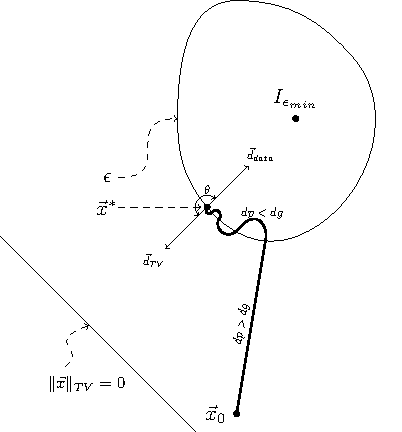
\includegraphics[scale=1.2]{RecAlgorithms/POCS.pdf} 
\end{center}

\caption[Diagram of the POCS algorithm]{\label{fig:POCSAlgo} Conceptual diagram of the ASD-POCS algorithm path to the solution.} 
\end{figure}


Figure \ref{fig:POCSAlgo} shows a conceptual diagram of the ASD-POCS algorithm. There is an area around the image with minimum data constrain, $I_{\epsilon_{min}}$. The solution $\vec{x}^*$ generally lies on the boundary of the area with the user specified $\epsilon$. From an initial image $\vec{x}_0$, the algorithm walks towards the area of acceptable $\epsilon$ more strongly than towards the area of minimum TV, as the step sizes of the vectors $\vec{d}_{\text{TV}}$ and $\vec{d}_{\text{data}}$, $dp$ and $dg$ respectively, are adaptively controlled to be $dp>dg$. Once the image is within acceptable 2 norm, then the step size is changed in order to have stronger $\vec{d}_{\text{TV}}$ ($dp<dg$). The optimal solution can be found when both vectors point in opposing direction, or in other words, when the angle between them is 180\ degrees, or the cosine of it is -1,

\begin{equation}
\cos \theta = \frac{\vec{d}_{\text{TV}} \cdot \vec{d}_{\text{data}}}{\lVert\vec{d}_{\text{TV}}\rVert \lVert\vec{d}_{\text{data}}\rVert }.
\end{equation}


The pseudocode for the algorithm can be seen in algorithm \ref{alg:ASD-POCS}. The algorithm is essentially solving the two vector in equation \ref{eq:KKTvectors}, the data vector in lines [5-8] and the TV vector in lines [18-22]. Line [9] enforces the positivity constrain. In the algorithm, $dtv$ is initialized according to $\alpha$, an user specified   TV hyperparameter for TV, together with $dp$, the step size performed by the data constrain. After the TV minimization is performed, the step size of the TV vector is rechecked. If the TV minimization step is too big (bigger than the data step size), and the desired $\epsilon$ is still not achieved, the step size is reduced further. This method of adaptively setting the step size of the TV iteration relating to the data step size is what ensures the optimal condition is achieved. Finally, the stopping criteria relies in either achieving the desired $\epsilon$ with with a desired $\cos \theta$, or stopping due to reaching a maximum amount of iterations ($\beta$ decreases with iteration number). In the original proposition of the ASD-POCS algorithm (and shown here), the data constrain is solved using SART, however any other algorithm solving the same minimization problem can be used here (e.g. CGLS or OS-SART).


The algorithm has 7 parameters that need to be set up: $\beta$ and $\beta_{red}$ are the initial value and reduction ratio of the SART hyperparameter, similarly $\alpha$ and $\alpha_{red}$ serve as hyperparameter and reduction ratio for the TV minimization. $r_{max}$ controls the maximum allowed ratio of change between the data minimization and the TV minimization, in order to adapt the step sizes. The number of iterations the TV minimization performs per iteration of the data minimization is defined as $n_{TV}$. Finally, the allowed data error is $\epsilon$, as described before. The initial values of the variables in the algorithm are a key factor on its convergence. Empirical tests show that wrong parametrization of the algorithm can lead to severely noisy reconstructions. An study of the sensitivity of these parameters to changes has been performed by Lohvithee \emph{et al}[CITE VEEs PAPER, at least as "future"]. The study shows that some parameters can be safely set up to a static value regardless of the data, such as the data hyperparameters, but that $\epsilon$, $n_{TV}$ and $\alpha$ are critical parameters to tune in order to get an usable reconstruction, and they are heavily data dependant. While some algorithms have successfully replaced the initial set of $\alpha$ by some data based heuristics [CITE PCSD]\footnote{These algorithms, namely PCSD and Aw-PCSD, are also available in TIGRE, by Manasavee Lohvithee.} to the best of the authors knowledge there is no mathematical proposal for setting these parameters. The biggest drawback of this method is that several reconstructions may be needed to find the best parameters for an specific application.

Note that this minimization approach, while used for TV minimization in the original article, can be used for a variety of different minimization functions. For example, the TV minimization step could be replaced by a prior image minimization[CITE PICS], or any other convex minimization function. Similarly, the data minimization step can be replaced by any other minimization algorithm, as long as it minimizes the problem in equation XX
\begin{algorithm}

\caption{ASD-POCS
\label{alg:ASD-POCS}}
\begin{algorithmic}[1]
\State{Set: $\beta, \beta_{red}, n_{TViter}, \alpha, \alpha_{red}, r_{max} $}
\State{$\vec{x}=0$};
\While{Stopping criteria not met}
\State $\vec{x}_{prev}=\vec{x}$
\For {$n_{angles}$}
\State  $\vec{x}=\vec{x}+\beta V A^T W^{-1} (\vec{b}-A\vec{x})$
\Comment SART update
\EndFor
\State $\beta=\beta*\beta_{red}$
\State $\vec{x}=\max(0,\vec{x})$
\Comment Enforce positivity
\State $\vec{x}_{out}=\vec{x}$

\State $\epsilon_{now}=\lVert A\vec{x}-\vec{b}\rVert$
\Comment Current $\epsilon$
\State $dp=\lVert\vec{x}-\vec{x}_{prev}\rVert$
\Comment Change in $\vec{d}_{\text{data}}$

\If {first iteration}
\State{$dtv=\alpha*dp$}
\Comment Initialize TV hyperparameter
\EndIf

\State $\vec{x}_{prev}=\vec{x}$
\State
\For {$n_{TViter}$}
\Comment TV update
\State $\vec{dx}= \nabla_{\vec{x}} \lVert\vec x \rVert_{TV}$
\State $\hat{dx}=\vec{dx}/\lVert\vec{dx}\rVert$
\State $\vec{x}=\vec{x}-dtv\cdot\hat{dx}$
\EndFor
\State $dg=\lVert\vec{x}-\vec{x}_{prev}\rVert$
\Comment Change in $\vec{d}_{\text{TV}}$
\If{$dg>r_{max}*dp$  \textbf{and} $\epsilon_{now}>\epsilon$}
\State $dtv=dtv*\alpha_{red}$
\EndIf
\State
\Comment Check stopping criteria
\State $\cos\theta=\vec{dp}\cdot\vec{dg}/\lVert\vec{dp}\rVert\cdot\lVert\vec{dg}\rVert$
\If {($\cos\theta<-0.9$ \textbf{and} $\epsilon_{now}<\epsilon$) \textbf{or} $\beta<0.005$}
\State Stop
\EndIf
\EndWhile

\end{algorithmic}

\end{algorithm}









\FloatBarrier
\subsubsection{The gradient of the TV norm}

In order to minimize the TV norm via gradient descend, the gradient of the TV norm needs to be computed, $ \nabla_{\vec{x}} ||\vec x ||_{TV}$, being $\vec x$ the vectorized form of a N-dimensional image.

The main challenge wit the $ \nabla_{\vec{x}} ||\vec x ||_{TV}$ term is that $ ||\vec x ||_{TV}$ is not differentiable in the general case. However, in the CT case, $\vec{x}$ can be described as $x_{ijk}$, a regularly discretized mesh of directional indices $i,j,k$ of maximum value $i_{max},j_{max},k_{max}$. The gradient of $x$ has an additional Cartesian index $\alpha$:

\begin{align}
g^\alpha &=\left(\nabla x\right)^\alpha=\partial_\alpha x\\
g^\alpha_{ijk} & = \partial_\alpha x_{ijk}.
\end{align}

The TV norm can me then defined as sum of the 2-norms of the gradient of $x$, $g$, over the Cartesian coordinate, resulting in a scalar.

\begin{align}
\lVert x \rVert_\text{TV}=\sum\limits_{ijk} \sqrt{\sum\limits_\alpha \left(g^\alpha_{ijk}\right)^2}=\sum\limits_{ijk} \sqrt{\sum\limits_\alpha \left(\partial_\alpha x_{ijk}\right)^2},
\end{align}

This is the term that the total variation regularization algorithm minimizes with a gradient descend. In order to perform this, the gradient of this term with respect to $x$ is needed, now defined in a scalar field
\begin{equation}
 (\nabla_{\vec{x}} || x ||_{TV})_{ijk}.
\end{equation} 

This derivative can be expanded to a 3 component value for each $x_{ijk}$ as:
\begin{align}
\left(\nabla_x \lVert x \rVert_\text{TV}\right)_{ijk}&= \frac{\partial}{\partial x_{ijk}} \lVert x \rVert_\text{TV} = \partial_{x_{ijk}} \sum\limits_{i^\prime j^\prime k^\prime} \sqrt{\sum\limits_\alpha \left(\partial_\alpha x_{i^\prime j^\prime k^\prime}\right)^2}\nonumber
\\
&= \sum\limits_{i^\prime j^\prime k^\prime} \partial_{x_{ijk}}\sqrt{\sum\limits_\alpha \left(\partial_\alpha x_{i^\prime j^\prime k^\prime}\right)^2} \nonumber \\ 
&=\sum\limits_{i^\prime j^\prime k^\prime} \frac{\sum_\alpha\left(\partial_\alpha x_{i^\prime j^\prime k^\prime}\right) \partial_{x_{ijk}} \left(\partial_\alpha x_{i^\prime j^\prime k^\prime}\right)}{\sqrt{\sum\limits_\alpha \left(\partial_\alpha x_{i^\prime j^\prime k^\prime}\right)^2}}.\label{eq:gradientTVdisc}
\end{align}

This term now contains $\partial_\alpha$ derivatives, i.e. derivatives in the Cartesian coordinate system $[x,y,z]$. These are defined as

\begin{align}
\partial_x x_{i^\prime j^\prime k^\prime} &= \lim\limits_{h\to 0} \frac{x_{i^\prime+h,j^\prime,k^\prime}-x_{i^\prime, j^\prime, k^\prime}}{h} \nonumber \\
\partial_y x_{i^\prime j^\prime k^\prime} &= \lim\limits_{h\to 0} \frac{x_{i^\prime,j^\prime+h,k^\prime}-x_{i^\prime, j^\prime, k^\prime}}{h} \nonumber \\
\partial_z x_{i^\prime j^\prime k^\prime} &= \lim\limits_{h\to 0} \frac{x_{i^\prime,j^\prime,k^\prime+h}-x_{i^\prime, j^\prime, k^\prime}}{h}.\label{eq:derivativedef}
\end{align}

However, $x$ is discrete, thus the limit definition of the derivative can not be used to numerically compute it, but an approximation of it can. By setting $h=1$, equation \ref{eq:derivativedef} becomes the backward finite differences of the first order approximation of a derivative, a very computationally cheap operation. The derivative w.r.t. the Cartesian coordinate can be rewritten as

\begin{align}
\partial_\alpha x_{i^\prime j^\prime k^\prime}=\delta_{\alpha x} \left(x_{i^\prime,j^\prime,k^\prime}-x_{i^\prime-1, j^\prime, k^\prime}\right)&+ \delta_{\alpha y} \left(x_{i^\prime,j^\prime,k^\prime}-x_{i^\prime, j^\prime-1, k^\prime}\right)  \notag \\ &+ \delta_{\alpha z} \left(x_{i^\prime,j^\prime,k^\prime}-x_{i^\prime ,j^\prime, k^\prime-1}\right)\
\end{align}
 where $\delta_\alpha$ is a Kronecker delta for the Cartesian axis. The other partial derivative term that appears in equation \ref{eq:gradientTVdisc} is $\partial_{x_{ijk}} \left(\partial_\alpha x_{i^\prime j^\prime k^\prime}\right)$. As the derivative is w.r.t. $x_{ijk}$, each component of $x$ is an independent variable, thus $\partial_{x_{ijk}} \left(\partial_\alpha x_{i^\prime j^\prime k^\prime}\right)$ is zero everywhere but in indices $i=i^\prime \wedge j=j^\prime \wedge k=k^\prime$, where the derivative is 1. The term then becomes 
 \begin{align}
\partial_{x_{ijk}} \partial_x x_{i^\prime j^\prime k^\prime}&=\partial_{x_{ijk}}\left(x_{i^\prime,j^\prime,k^\prime}-x_{i^\prime-1, j^\prime, k^\prime}\right)=\delta_{i^\prime,i}\delta_{j^\prime,j}\delta_{k^\prime,k} - \delta_{i^\prime-1,i}\delta_{j^\prime,j}\delta_{k^\prime,k}\nonumber\\
&=\delta_{i^\prime,i}\delta_{j^\prime,j}\delta_{k^\prime,k} - \delta_{i^\prime,i+1}\delta_{j^\prime,j}\delta_{k^\prime,k}\nonumber\\
%
\partial_{x_{ijk}} \partial_y x_{i^\prime j^\prime k^\prime}&=\partial_{x_{ijk}} \left(x_{i^\prime,j^\prime,k^\prime}-x_{i^\prime, j^\prime-1, k^\prime}\right)=\delta_{i^\prime,i}\delta_{j^\prime,j}\delta_{k^\prime,k} - \delta_{i^\prime,i}\delta_{j^\prime-1,j}\delta_{k^\prime,k}\notag\\
&=\delta_{i^\prime,i}\delta_{j^\prime,j}\delta_{k^\prime,k} - \delta_{i^\prime,i}\delta_{j^\prime,j+1}\delta_{k^\prime,k}\nonumber\\
%
\partial_{x_{ijk}} \partial_z x_{i^\prime j^\prime k^\prime}&=\partial_{x_{ijk}} \left(x_{i^\prime,j^\prime,k^\prime}-f_{i^\prime, j^\prime, k^\prime-1}\right)=\delta_{i^\prime,i}\delta_{j^\prime,j}\delta_{k^\prime,k} - \delta_{i^\prime,i}\delta_{j^\prime,j}\delta_{k^\prime-1,k}\notag\\
&=\delta_{i^\prime,i}\delta_{j^\prime,j}\delta_{k^\prime,k} - \delta_{i^\prime,i}\delta_{j^\prime,j}\delta_{k^\prime,k+1}.
\end{align}

These terms are practically a selecting function for $i^\prime ,j^\prime ,k^\prime$ ,matching only in the indices $i,i+1,j,j+1,k,k+1$ in the sum of the right hand side of equation \ref{eq:gradientTVdisc}. However the indices are limited to $i^\prime \in [1,i_{max}]$, $j^\prime \in [1,j_{max}]$ and $k^\prime \in [1,k_{max}]$. As boundary conditions, Neumann boundary conditions are set to zero. To enforce that, a Kronecker deltas can be introduced for each index, $\left(1-\delta_{i,i_{max}}\right)$, with the same approach with the other indices.

Finally, substituting in equation \ref{eq:gradientTVdisc}, the gradient of the TV norm can be described as

\begin{align}
&\left(\nabla_x \lVert x \rVert_\text{TV}\right)_{ijk}=\sum\limits_{i^\prime j^\prime k^\prime} \frac{\sum_\alpha\left(\partial_\alpha x_{i^\prime j^\prime k^\prime}\right) \partial_{x_{ijk}} \left(\partial_\alpha x_{i^\prime j^\prime k^\prime}\right)}{\sqrt{\sum\limits_\alpha \left(\partial_\alpha x_{i^\prime j^\prime k^\prime}\right)^2}}\notag\\
&=\sum\limits_{i^\prime j^\prime k^\prime} \frac{\partial_x x_{i^\prime j^\prime k^\prime} \partial_{x_{ijk}} \left(\partial_x x_{i^\prime j^\prime k^\prime}\right) + \partial_y x_{i^\prime j^\prime k^\prime} \partial_{x_{ijk}} \left(\partial_y x_{i^\prime j^\prime k^\prime}\right) + \partial_z x_{i^\prime j^\prime k^\prime} \partial_{x_{ijk}} \left(\partial_z x_{i^\prime j^\prime k^\prime}\right)}{\sqrt{\sum\limits_\alpha \left(\partial_\alpha x_{i^\prime j^\prime k^\prime}\right)^2}}\notag \\
&=\frac{\partial_x x_{i,j,k}+\partial_y x_{i,j,k}+\partial_z x_{i,j,k}}{\sqrt{\sum\limits_\alpha \left(\partial_\alpha x_{i, j, k}\right)^2}}\notag \\
& - \frac{\left(1-\delta_{i,i_{max}}\right) \partial_z x_{i+1,j,k}}{\sqrt{\sum\limits_\alpha \left(\partial_\alpha x_{i+1, j, k}\right)^2}} - \frac{\left(1-\delta_{j,j_{max}}\right) \partial_y x_{i,j+1,k}}{\sqrt{\sum\limits_\alpha \left(\partial_\alpha x_{i, j+1, k}\right)^2}} - \frac{\left(1-\delta_{k,k_{max}}\right) \partial_z x_{i,j,k+1}}{\sqrt{\sum\limits_\alpha \left(\partial_\alpha x_{i, j, k+1}\right)^2}}.\label{eq:gradientTVnormNumerical}
\end{align}

Equation \ref{eq:gradientTVnormNumerical} is the numerical approximation of the gradient of the total variation norm, and describes scalar field of the same size of the image. The same approach can be used with central and forward differences to obtain a similar equation, however central differences may not correctly minimize the TV norm of the image. As central differences do not take into account the value of the current voxel $ijk$, a chequerboard pattern would have zero TV norm, and this is the opposite of the purpose of the algorithm, therefore only numerical approximations of derivatives that take immediately adjacent pixel values into account can be used (such as forward or backward finite differences).

\subsection{Total variation regularization via Rudin-Osher-Fatemi model} \label{sec:SART-TV}

A different minimization approach to POCS is the approach proposed by Jia \textit{et al}\cite{jia2011gpu}, that uses the Rudin-Osher-Fatemi (ROF) model for total variation minimization, widely used in the denoising literature\cite{RUDIN}\cite{duran2013chambolle}\cite{vogel1996iterative}. By starting from the same minimization problem, namely
\begin{equation}
\hat{x}=\argmin_x \lVert Ax-b \rVert^2+\lambda \lVert x\rVert_{TV},
\end{equation}
and a forward-backward splitting algorithm\cite{combettes2005signal} is used to split the minimization into two alternating steps, the TV and the data steps. If the optimality condition is considered to be
\begin{equation}
\frac{\partial}{\partial x_\alpha}\lVert Ax-b \rVert^2+\lambda\frac{\partial}{\partial x_\alpha}\lVert x\rVert_{TV}=0,
\end{equation}
being $\alpha$ the set of Cartesian coordinates, then the problem can be split into the following equations, where $g$ is a auxiliary function and $\mu>0$:
\begin{align}
\lambda\frac{\partial}{\partial x_\alpha}\lVert x\rVert_{TV}=\mu (x-g)\\
\frac{\partial}{\partial x_\alpha}\lVert Ax-b \rVert^2=-\mu (x-g).
\end{align}

By solving for $g$, the simplified version of the algorithm can be seen in \ref{alg:SART-TV}.

\begin{algorithm}
\caption{TV minimization with ROF model
\label{alg:SART-TV}}
\begin{algorithmic}[1]
\State Solve: $g=x-\frac{\lambda}{\mu} \frac{\partial}{\partial x_\alpha}\lVert Ax-b \rVert^2$
\Comment SART
\State Minimize: $x=\argmin_x  \lVert x\rVert_{TV}+0.5*\mu \lVert x-g \rVert^2$

\State Enforce positivity: $x=\max(0,x) $
\end{algorithmic}

\end{algorithm}

The first line of the algorithm its essentially a gradient descend iteration, which is essentially a SART iteration. Note that the SART iteration can be replaced by other data-minimization algorithms such as CGLS. The second line is the ROF model, widely researched in image denoising. The ROF model tries to find the image $x$ with minimum total variation subject to having the minimal deviation from its original value $g$. By changing the value of he hyperparameter $\mu$, the strength of this regularization is controlled. A high $\mu$ will ensure that the image is very similar to its original value, while a small $\mu$ will be more lax. The advantage of this approach compared to the ASD-POCS algorithm is that it requires no extra projection or backprojection operations. Additionally, minimizing the ROF model is a very well studied problem in the image processing field, and it has lead to finding computationally efficient methods.

 In the article by Jia \emph{et al}, they solve the ROF model via gradient descend and controlling its step size with Armijo's rule. In this work a different approach is taken, based on the image processing literature.
 
 \subsubsection{Primal Dual formulation of the ROF model}
 
As previously shown in line 2 of algorithm \ref{alg:SART-TV}, the ROF model can be formulated as 
\begin{equation}
\hat{x}_{ROF}=\argmin_x  \lVert x\rVert_{TV}+\frac{\mu}{2} \lVert x-g \rVert^2.\label{eq:ROF}
\end{equation}

A solution of this problem using a primal-dual (PDU) approach has been proposed in literature\cite{zhu2008efficient}, by changing the minimization equation to a saddle point optimization problem. While a wide variety of methods have been proposed to minimize the ROF model\cite{RUDIN}\cite{vogel1996iterative}\cite{chambolle2004algorithm}, the PDU method has the advantage of being very parallelizable, thus a perfect fit for GPU computing. The dual variable can be proposed by using the TV definition of $\lVert x\rVert_{TV}=\lVert \nabla x \rVert$ and observing the following consequence of the Cauchy-Schwartz inequality

\begin{equation}
\lVert \nabla x \rVert=\argmax_{\lVert\textbf{p}\rVert\leq 1} \lVert\textbf{p}\nabla x\rVert,
\end{equation}
where $\textbf{p}=(p^1,p^2,p^3)^T$ (for the 3D case) is the said dual variable. Note that each $p^i$ is the size of the image $x$. Equation \ref{eq:ROF} can be then rewritten as
\begin{equation}
\hat{x}_{ROF}=\argmin_x \argmax_{\lVert\textbf{p}\rVert\leq 1}\lVert\textbf{p}\nabla x\rVert + \frac{\mu}{2} \lVert x-g \rVert^2.\label{eq:PUD}
\end{equation}

The primal and dual updates can be both obtained from this equation. For the primal update, differentiating the equation according to $x$ results in
\begin{equation}
- \nabla \cdot\textbf{p}+\mu(x-g)=0,
\end{equation}
and one can solve it for $x$ by performing a gradient descend update as
\begin{equation}
x^{n+1}=x^n(1+\tau_P^n)+\tau_P^n\left(g+\frac{1}{\mu} \nabla \cdot \textbf{p}\right),
\end{equation}
where $\tau_P$ is the primal step size. The dual update can be computed similarly, by differentiating equation \ref{eq:PUD} according to $\textbf{p}$, the following equation si obtained:
\begin{equation}
\nabla x+\textbf{p}\alpha=0,
\end{equation}
where $\alpha$ is a Lagrange multiplier for the inequality constrain $\lVert\textbf{p}\rVert\leq 1$. This equation can be maximized with a gradient ascend method as
\begin{equation}
\textbf{p}^{n+1}=\Pi_{B_0}\left(\textbf{p}^{n} +\tau_D^n\nabla x\right),
\end{equation}
where $\Pi_{B_0}(\textbf{p})=\frac{\textbf{p}}{\max\{1,\lVert\textbf{p}\rVert\}}$ is a projection onto the unit ball centred in the origin.

The PDU algorithm consists in updating $\textbf{p}$ and $x$ iteratively, by alternating the updates. In \cite{zhu2008efficient}\cite{knoll2010fast} a step size update is proposed for the primal and dual step sizes:
\begin{align}
&\tau_D^n=0.3+0.02n \notag \\
&\tau_P^n=\frac{1}{\tau_D^n}\left(\frac{1}{6}-\frac{5}{15+n}\right).
\end{align}

The same update is used in this work, as the images in their work are structurally similar to CT images and empirical test showed satisfactory results. The algorithm can be shown to converge as it is shown in \cite{zhu2010duality} that the primal-dual gap decreases with each update of $x^n$, and the gap is suggested as a control variable for the stopping criteria. In this work the algorithm has been implemented without the stopping criteria check, and an user specified parameter for the number of iterations is passed as an input, with a default value of 50, as it empirically showed good results.

The discretization of the divergence and gradient operators are a key factor when numerically computing the PDU algorithm, as they need to be consequent with each other. Thus, the gradient can be approximated using forward differences, but as the divergence is the adjoint of the gradient, it must be approximated with backwards differences.






\section{Discussion}
\label{ch:rec}


% !TeX root = c:/Latex/Thesis/main.tex

\chapter{GPU methods in tomography}

Tomographic reconstruction in 3D is not only challenging due to the mathematics of the reconstruction, but also comes with a significant computational burden. As an example, the detector may have $512^2$ pixel per projection and the size of the reconstructed image is generally of the order of $512^3$ voxels in medical applications. However, in micro-tomography the detectors can get to sizes such as $2000^2$ pixels per angle with images of $2000^3$ voxels. Such sizes are considerably big for standard computers and applying reconstruction techniques. Both ``one pass'' as FDK or iterative methods are massively computationally expensive, needing up to weeks to reconstruct the image if run on CPUs. This is in most cases an unreasonable waiting time, as images are required for immediate  diagnosis or treatment adjustment when taken, so a faster solution is needed.

In iterative reconstruction techniques, the computational problem relies on the matrix $A$, generally used twice per iteration in most algorithms, by doing a projection ($A\cdot x$) and a backprojection ($A^T\cdot b$). The construction of this matrix is not possible in 3D tomography, due to its size. If we consider the medical case sizes presented before, with projections over 360 different angles, building explicitly the $A$ matrix would require thousands of gigabytes of RAM memory just to store the $0.0017\%$ of the matrix that has non-zero values. In order to avoid that, the common technique is to compute $A\cdot x$ and $A^T\cdot b$ as a single operation instead of computing $A$ explicitly. This is possible because the matrix-vector operation $A\cdot x$ describes the result of the integral of the x-rays over the image and $A^T\cdot b$ describes a ``smear'' of the projection data onto the image in the corresponding voxels. Interestingly, both of this operands necessitate a massive amount of very independent and simple calculations.

Over the past years computational technology has evolved significantly. But Moore's law, which expresses the halving of transistor size every two years, is coming to an end due to physical laws. Transistors  are currently on the 14nm scale and, while they are expected to reach 5nm by 2020, this clearly already breaks Moore's law. As transistors reach this scale, quantum mechanics starts to have an important effect, especially quantum tunnelling where the electrons could just ``jump''\footnote{Explanations about quantum mechanics are far beyond the goals of this thesis.} to the other side of the transistor regardless of its state. Unless a breakthrough in the understanding and manufacturing of new materials that can overcome such effects is discovered, 5nm transistors is approximately the hard limit to how far processors can evolve. To overcome this limitation, research in different computer architectures has been a hot topic in the past decades. This lead to two separate, but similar advances: High Performance Computers (HPCs) and Graphic Processing Units (GPUs). HPCs developed in order to be able to accommodate the growing computational demands of researchers and industry, where big data and heavy parallel computations became more common. These are massive installations with an enormous power consumption and running costs. GPUs instead, advanced their technology in order to accommodate the more demanding graphic (or visual) specifications of mainly the video-game industry in personal computers. GPUs are intrinsically designed to run in personal devices, such as laptops or mobile phones, so they are designed to be not only fast but small, low consumption and cheap overall.

The computations on high-end graphics in video-games require similar algorithms and processes than some of the big computational problems in both industry and research. It turns out that the development of high throughput GPUs for video-games has brought a tool that can significantly help research methods nowadays, to the point that a new term has been coined: GPGPUs or General Purpose GPUs. GPGPUs are widely used in research, for example in molecular dynamic simulations\cite{phillips2005scalable}, astrophysical hydrodynamics\cite{CHOLLA}, artificial intelligence\cite{Tensorflow}, and many more. The massively parallel architecture and large number of independent processors make GPGPUs the perfect tool to deal with computed tomography applications.

%This chapter describes the core code that underpins the TIGRE (\textbf{T}omographic \textbf{I}terative \textbf{G}PU-based \textbf{Re}construction) Toolbox\cite{TIGRE}, a free MATLAB-CUDA toolbox for fast tomographic iterative reconstruction algorithms. First, a further description of the GPU architecture is given. Then, the special features of these processors that make tomography, and especially iterative reconstruction algorithms, a good fit for GPGPUs is shown. Next, a detailed description is given of how the projection operator has been implemented and optimized, followed by a similar description for the backprojection operator. Once all the optimization tricks have been presented, a detailed analysis of the performance of the code is given showcasing the speeds achieved and the places were improvements could be made. After the computational aspects of the code, the general design of the TIGRE toolbox is described linking the computational research from this chapter to the algorithmic and mathematical methods from Chapter 3. Finally, a summary of the research is discussed and a brief comparison with other available software for GPU X-ray reconstruction is given. 

This chapter describes the core computational code used in this work. First, a further description of the GPU architecture is given. Then, the special features of these processors that make tomography, and especially iterative reconstruction algorithms, a good fit for GPGPUs is shown. Next, a detailed description is given of how the projection operator has been implemented and optimized for two different projection approaches.  And finally, a similar description for both of the backprojection modes implemented is given.


This chapter focuses on CBCT geometry, but parallel geometries are also implemented in the code. Everything (both computational and algorithmic) discussed for CBCT is essentially the same for any other geometry, with some minor tweaks applied. All the methods discussed in this section and in the TIGRE toolbox are available open source and free to use/access in the paper\cite{TIGRE} and GitHub repository \href{https://github.com/CERN/TIGRE}{github.com/CERN/TIGRE}.

\section{Hardware used in this research}
Prior to the description of hardware architectures and programming tricks, it is important to describe the hardware that this research was developed on. While the work presented here applies to almost all different hardware types, it may not be 100\% applicable to any GPU. GPUs are constantly changing so some features and computational tricks used for the acceleration of CT code are recent additions to GPGPUs and similarly new improvements to GPGPUs will come in the future that may render obsolete the information presented in this chapter. Therefore, this work presents techniques and benchmarks based on the hardware that was available and, while most of the techniques are applicable to most of GPUs, the mileage may vary. Additionally, most of the terminologies used in this chapter are related with NVIDIA/CUDA.

The research on this (and further) chapters of this thesis has been performed on a PC with a Windows 7 x64 operating system, with 32Gb of on board RAM, and a SSD hard drive. The GPU used was a NVIDIA Tesla 40k, that has 2880 stream processors, a clock frequency of 745-875 MHz and an on board RAM of 12GB. The processing power is generally described in terms of floating-point operations per second or FLOPS, and this particular GPU has a theoretical throughput of 4.29-5.04 TFLOPS on single-precision numbers.

\section{GPGPU architecture}

In order to better describe how GPU acceleration boosts tomographic reconstruction, a description of the hardware architecture of GPUs is required. As previously mentioned, GPUs are a technology that evolved from the increasing requirements of the entertainment industry in general but particularly from video games. In order to be able to have more realistic real-time graphics, where the environment reacts to the user interface by changing light reflections, textures, and simulating the physics of objects, a high throughput hardware is required. All these effects need a large amount of simple arithmetic to be computed and a fast access memory, faster than any modern CPU can handle. For that reason computers started having GPUs, special dedicated hardware that included hundreds of small, low-power, low-speed processors. These processors are significantly worse than any CPU, but the high number of them allows very high throughput for any arithmetically heavy algorithm. However, this high computation-intensive output design also means that GPUs perform weakly on programs that need control flow and caching. This information is key for the correct design of GPU algorithms as will become more evident further in this chapter.

The general diagram of the GPU architecture is presented in figure \ref{fig:GPUarch}. It has 3 main parts, the computational core, the device memory (DRAM) and the communication with the CPU via PCI express (PCIe).
The principal part of the GPU is the computational part. This consists of several stream multiprocessors (SMs), 15 in the Tesla k40, that are responsible for the distribution of the instructions to the stream processors (SPs) or CUDA cores. Each of the SPs (2880 in total) can run a single \textit{block} of instructions at any time, each of them consisting of up to 1024 parallel\footnote{In GPU computing, one should not confuse \textit{parallel} with \textit{concurrent}. Parallel means that the same instruction is divided into pieces, but they are not necessarily executed at the same time.} \textit{threads}. These blocks must be running the same algorithm, or \textit{kernel}. Theoretically, each of the SPs can have 64 \textit{concurrent warps}, or execution instructions running at the exact same clock cycle, each of these warps having 32 threads. This means that the Tesla k40 can have a theoretical maximum of 30720 arithmetic operations simultaneously executing. This is never reached as some of this time may be spent in flow control or memory reads, thus slowing the execution. 

\begin{figure}
\begin{center}

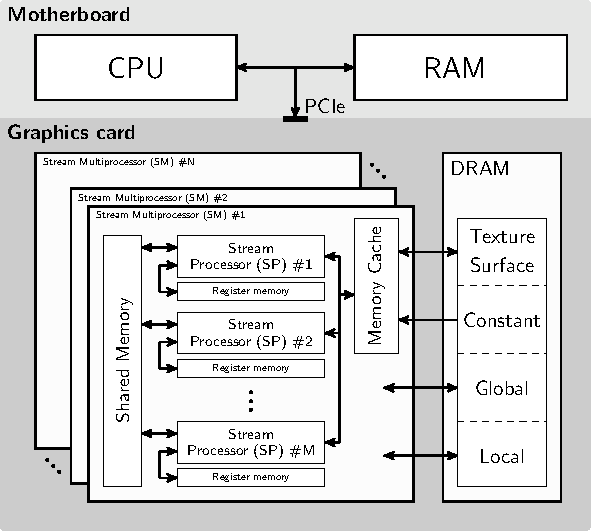
\includegraphics[width=\textwidth]{GPUmethods/architecture-figure0.pdf} 
\end{center}

\caption[Block diagram of a GPU architecture]{\label{fig:GPUarch} Diagram of a the basic architecture of a GPU. It shows how processing units and memory is structured inside a graphics card.} 
\end{figure}



The second part of the GPU are the memory types. There are 3 types of memory in the GPU: registers, shared memory and device random access memory (DRAM). The main difference between them is in accessibility (what subset of the SPs can access it) and speed. The lowest level memory is register memory. This is a thread level memory, used to store all local variables during execution. It is fast access and low in size. No other thread or block can access this memory. The second memory type is shared memory. This memory is used when blocks need to share information, such as the result of a computation in the middle of the kernel. Each SM has its own shared memory and it is local to them. All blocks can access to it, but careful usage of it is needed as the parallel nature of the computation could mean multiple writing on the same memory by different blocks. This memory is bigger (up to 48KB) and it is fast access, but slower than registers. Finally, there is DRAM memory. DRAM memory is a global large (12GB) memory on the board. This memory is widely used as it is the place where memory before kernel calls is allocated and where the results are stored after kernel calls. However, GPU code will often need to work with big data, thus the DRAM read/write is also commonly used within kernels. DRAM accessing can lead to significant bottlenecks as a single memory access needs 200 to 300 clock cycles to be carried. 

To improve memory throughput, the GPU contains so-called L1/L2 cache memory on each of the SMs. This cache is designed to improve execution of \textit{memory coalescing} warps. The cache, having a faster communication bus with the threads (needing about 80 cycles for a single memory read) stores a large amount of memory each time a single read to the DRAM is performed. The memory is loaded with locality, i.e., a memory chunk around the first sampled value is loaded, as the cache expects subsequent memory reads to be adjacent. Thus, when designing kernels, the order of the memory access can have a big influence on the final speed of the program. 

Two memory types can be used when data locality needs to be exploited in cache access: texture and surface memory. The difference between them is that the former is read only while the later can also be written. These memories can be defined as 3D shaped, thus data locality can be exploited in all spatial dimensions. Additionally, both can be accessed with floating point index values, and the memory value is returned with user-chosen interpolated methods. If cached memory is desired, but not in a spatially correlated form, then the read only constant memory can be used. This memory is still cached and can be used to speed up values that may be needed often. Then there is the global memory, which is read and write but not cached. Finally, local memory is an extension of shared memory when it gets filled.

The third important section is the communication between CPU-GPU. This is done via PCI-express ports and it is a slow communication process. Passing data from CPU to GPUs is relatively fast (500Mb/s), but can be a bottleneck in memory-heavy applications such as CT imaging.



\subsection{Exploiting GPGPUs for CT}

In CT, two main operations need to be accelerated: projection and backprojection. While iterative algorithms are defined as algebraic methods using a big system matrix $A$, the matrix itself is rarely used alone in the equations, it is generally used as $A*x$ or $A^T*b$. Fortunately, these two operations have a physical meaning, as the projection is the integral of the image over the straight X-ray paths, and the backprojection is the ``smearing'' of the detector data over the image back in the direction of the source, also following straight paths. While computing the values of the rows and columns of the system matrix seems hardly possible in real time, these two operations can be performed abstracting from their algebraic equivalent. The projection operation is an integration over independent, yet closely related, straight paths. By being able to sample the image domain in parallel, the operation can be performed at high speed. Similarly, the backprojection relies on building straight lines from the source to the voxels or detectors (dependent on the backprojection type), and sampling the projections. These operations are completely independent, hence the idea for GPU parallelism as threads will reach their maximum performance when they do not need to communicate with each other.  Additionally, both operations need accurate sampling over large volumes, thus texture memory with interpolation is ideal as it is hardware optimized, giving faster interpolated values than in a CPU or any possible interpolation kernel. Therefore the massive parallelism and texture memory are they key features of GPU computing that make it the ideal tool for accelerating tomography. The following sections provide more details.

\section{The projection operator}
The projection operator is the numerical equivalent of the X-ray integral that defines the model of X-ray tomography (see equation XX). This operator models the idealized physics, where all the X-rays have an infinitely small width and travel in a straight path to the center of each detector pixel, and all with the same energy. While this may not represent the physics accurately enough to be a reliable X-ray  simulation tool, it is exactly what iterative methods need, the $A*x$ operation. 


There are several method to simulate forward projection, all of them easily parallelizable. One of these is the distance-driven projection \cite{BrunoDeMan}\cite{schlifske2016fast}, where the ray-voxel and detector intersections are all projected in a mid-plane and values are accumulated there. Alternatively, the voxel-driven projector\cite{Du2017}, where the whole voxel (square or other shape\cite{lewitt1992alternatives}) is projected onto the detector and its values spread among all the corresponding pixels. With a similar approach, the separable footprints technique\cite{long20103d}\cite{wu2011gpu} approximates the footprint of the voxel in the detector for speed-up.  According to the authors it is more accurate than the distance-driven projection and faster than both the voxel-driven and distance-driven ones. Finally, in ray-driven projection\cite{siddon1985fast}\cite{xu2010fast}\cite{chou2011fast} methods the line path is integrated. Among these, the most important variations worth mentioning are the infinitesimally small exact path, area path, and the grid-interpolated path. The exact path computes either the length of an infinitesimally narrow path or the area of a finite width path over each voxel and uses that as a weight for the integral. The grid-interpolated projector instead sets a fixed sample length and interpolates voxel values. According to a study by Fang and Mueller\cite{1625152}, the most accurate methods are the ray-driven ones.

This work has focused on the infinitesimally small ray-voxel intersection and grid-interpolated methods only because in both the desired accuracy and speed have been reached. The grid-interpolated method also is a key method for the following chapters (see Chapter 6 for more information). As the projection is basically an integral of a volume over thousands of independent paths, it is straightforward to parallelize by independently computing each ray. The ray-voxel intersection method is equivalent to the algebraic representation, where the $A$ matrix contains the length of the intersection between voxels and the path. Those are multiplied and added to the voxel values themselves to obtain the detector values. However, while not feasible in CPUs, the grid-interpolated method can use the practically free (i.e., very little time overhead) texture memory interpolation for speed-up in GPUs. The difference between the methods can be seen in figure \ref{fig:Amatrix}. 

\begin{figure}

\begin{center} 
\subfigure[]{ 
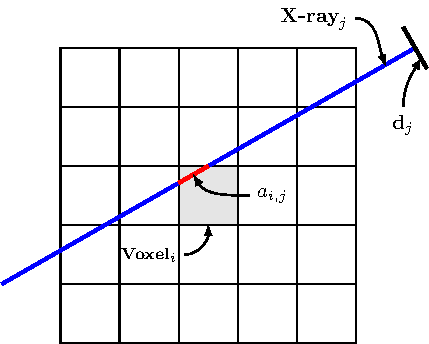
\includegraphics[width=0.45\linewidth]{GPUmethods/Amatrix-siddon.pdf} 
\label{fig:AmatrixSiddon} 
}
\subfigure[]{ 
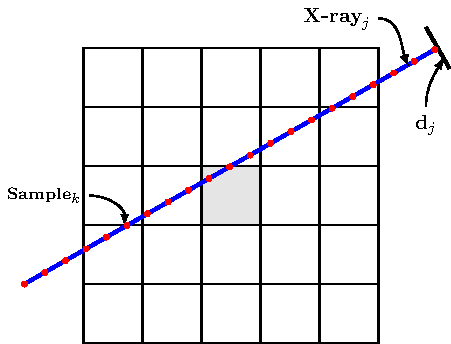
\includegraphics[width=0.45\linewidth]{GPUmethods/Amatrix-interp.pdf} 
\label{fig:AmatrixInterp} 
}
 
\caption[Diagram of projection types]{\label{fig:Amatrix}(a) Diagram of the projection operation using the line-voxel intersection methods and (b) diagram of the interpolated sampling method.} 
\end{center} 
\end{figure}

\FloatBarrier

\subsection{Ray-voxel intersection method}

As previously mentioned, this method relies on accumulating the length of the intersection between a straight path and voxels multiplied by the voxel value. The X-ray integral from equation XX can be discretized as in equation \ref{eq:ray-voxel}, where $d_{uv}$ is the detector value of X-ray $uv$, $\mathbb{I}(ijk)$ are the voxel values of the image and $l_{uv,ijk}$ the length of the path within each voxel. Note that here $l_{uv,ijk}$ are the same values as the elements of matrix $A$. Computing $l_{(uv,ijk)}$ requires some geometrical computations, not only the reliable detection of the intersections between the lines and voxel boundaries, but also avoiding computing it on voxels where the line does not intersect.

\begin{equation}
d_{(uv)}= \sum_{ijk=0}^{N_\mathbb{I}}l_{(uv,ijk)}*\mathbb{I}(ijk)
\label{eq:ray-voxel}
\end{equation}


\begin{figure}
\begin{center}

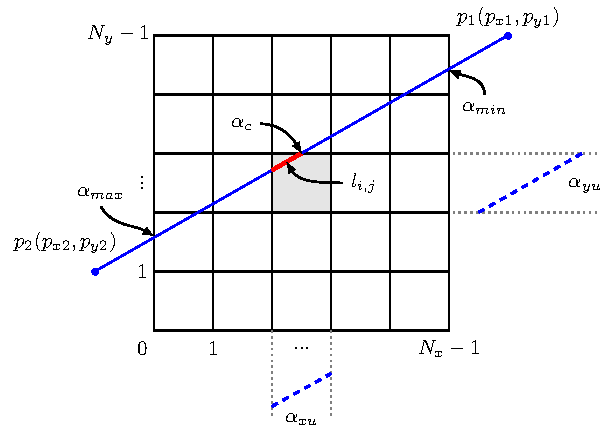
\includegraphics{GPUmethods/Amatrix_siddon_diagram.pdf} 
\end{center}

\caption[Jacob's ray tracing diagram]{\label{fig:Siddon} Diagram of the relevant variables for Jacobs' ray-tracing algorithm.} 
\end{figure}



The algorithm to compute $d_{uvj}$ has been taken from Jacobs\cite{jacobs1998fast} improvement on Siddon's method\cite{siddon1985fast}. For the sake of clarity, the algorithm is described for the 2D case, but the extension to 3D is trivial. The algorithm is based on computing the intersection between the path and the x and y planes and iterating over the ray until the next intersection is found. The diagram of the variables used in the algorithm can be seen in figure \ref{fig:Siddon}. The following derivation assumes that the pixels are of size 1 and the image domain starts at $(0,0)$, as this assumption reduces the number of operations needed. Assuming non-trivial rays from point $(p_{x1},p_{y1})$ to point $(p_{x2},p_{y2})$, the parametric representation of the ray is
\begin{equation}
p_{12}=
\begin{cases}
      p_x(\alpha)&=p_{x1}+\alpha (p_{x2}-p_{x1})\\
      p_y(\alpha)&=p_{y1}+\alpha (p_{y2}-p_{y1}),\label{eq:line}
    \end{cases}
\end{equation}
where $\alpha \in [0,1]$. In order to know the number of intersections, the initial and final intersections of the ray in the image are needed. The intersection points in terms of alpha can be defined as
\begin{equation}
\alpha_x(i) = \frac{(i-p_{x1})}{p_{x2}-p_{x1}}\label{eq:alphax}
\end{equation}
\begin{equation}
\alpha_y(j) = \frac{(j-p_{y1})}{p_{y2}-p_{y1}},\label{eq:alphay}
\end{equation}
where $i$ and $j$ are indices of the pixels. If the number of planes is defined as $N_x$ and $N_y$, one can compute the minimum and maximum $\alpha$ values (i.e., values of the line at the boundary of the image) by comparing the values of $\alpha$ in each direction as

\begin{align}
\alpha_{min}&=\max \Big(\min \big(\alpha_x(0),\alpha_x(N_x-1)  \big), \min \big(\alpha_y(0),\alpha_y(N_y-1)  \big) \Big)\\
\alpha_{max}&=\min \Big(\max \big(\alpha_x(0),\alpha_x(N_x-1)  \big), \max \big(\alpha_y(0),\alpha_y(N_y-1)  \big) \Big).
\end{align}
Note that this is equivalent to writing

\begin{align}
\alpha_{min}&=\max \Big( \alpha_{xmin},\alpha_{ymin} \Big)\\
\alpha_{max}&=\min \Big( \alpha_{xmax},\alpha_{ymax}\Big).
\end{align}

Next, the planes where the rays first cross in each direction need to be computed. This can be achieved by looking at the different $\alpha$ values. For the $x$ dimension, equations \ref{eq:alpha1-1}-\ref{eq:alpha1-2} show how to compute the plane index $i_{min}$ and $i_{max}$ if $p_{x1}<p_{x2}$ and equations \ref{eq:alpha2-1}-\ref{eq:alpha2-2} when $p_{x1}>p_{x2}$. The same logic applies to $j_{min}$ and $j_{max}$.

\begin{align}
\alpha_{min}&=\alpha_{xmin}\quad \rightarrow\quad i_{min}=1 \label{eq:alpha1-1}
\\
\alpha_{min}&\neq\alpha_{xmin}\quad \rightarrow\quad i_{min}=\lceil{ p_x(\alpha_{xmin})}\rceil \\
\alpha_{max}&=\alpha_{xmax}\quad \rightarrow\quad i_{max}=N_x-1\\
\alpha_{max}&\neq\alpha_{xmax}\quad \rightarrow\quad i_{max}=\lfloor{ p_x(\alpha_{xmax})}\rfloor 
\label{eq:alpha1-2}
\end{align}
\begin{align}
\alpha_{min}&=\alpha_{xmin}\quad \rightarrow\quad i_{max}=N_x-2 \label{eq:alpha2-1}\\
\alpha_{min}&\neq\alpha_{xmin}\quad \rightarrow\quad i_{max}=\lfloor{ p_x(\alpha_{xmin})}\rfloor \\
\alpha_{max}&=\alpha_{xmax} \quad\rightarrow\quad i_{min}=0\\
\alpha_{max}&\neq\alpha_{xmax} \quad\rightarrow\quad i_{max}=\lceil{ p_x(\alpha_{xmax})}\rceil .
\label{eq:alpha2-2}
\end{align}

At this point, the $\alpha_x$ and $\alpha_y$ values of the first intersection point can be obtained by substituting either $(i_{min},j_{min})$ or $(i_{max},j_{max})$ (depending on the relationship of $p_1$ and $p_2$) into equations \ref{eq:alphax} and \ref{eq:alphay}. Additionally, one can compute the number of planes that the ray crosses ($N_p$) with the following equation:
\begin{equation}
N_p=(i_{max}-i_{min}+1)+(j_{max}-j_{min}+1).
\end{equation}

In order to be able to start iterating over a given line there are just two pieces of information missing, namely the initial pixel coordinates and the $\alpha_u$, the maximum step in each direction for a unit of change. The initial pixel coordinates can be computed as

\begin{align}
i&=\bigg\lfloor{p_x\Big(\frac{min(\alpha_x,\alpha_y)+\alpha_{min}}{2}\Big)}\bigg\rfloor\\
j&=\bigg\lfloor{p_y\Big(\frac{min(\alpha_x,\alpha_y)+\alpha_{min}}{2}\Big)}\bigg\rfloor.
\end{align}

The maximum $\alpha$ that can happen in a unit of change in each direction, or $\alpha_{xu}$ and $\alpha_{yu}$ are defined as in equation \ref{eq:unitalpha}. Additionally it is useful to have a variable that controls the unit direction of the ray, $i_u$ and $j_u$, as in equation \ref{eq:direction}.

\begin{equation}
\alpha_{xu}=\frac{1}{\left|p_{x2}-p_{x1} \right|}\label{eq:unitalpha}
\end{equation}
\begin{equation}
i_u=
\begin{cases}
1 & \text{if}\quad p_{x1}< p_{x2}\\
-1 &\quad\quad\text{otherwise}
\end{cases}\label{eq:direction}
\end{equation}

Defining $l_{tot}$ as the Euclidean distance between $p_1$ and $p_2$ and initializing the current $\alpha$, $\alpha_c=\alpha_{min}$, the iterative method to follow the X-ray path can be described as follows. Check if the next intersection is in $x$ or $y$ by comparing the $\alpha$ values of each direction, then choose to update the direction that has a smallest $\alpha$. When updating, compute the length of the next distance and update the $\alpha$, pixel index and integral values. The update when $\alpha_x<\alpha_y$ can be seen in equations \ref{eq:siddonUpdatex1}-\ref{eq:siddonUpdatex2}, and the opposite case in equations  \ref{eq:siddonUpdatey1}-\ref{eq:siddonUpdatey2}.
\begin{align}
d_{ray}\quad&=\quad d_{ray}+(\alpha_x-\alpha_c)\cdot l_{tot} \cdot\mathbb{I}(i,j)\label{eq:siddonUpdatex1}\\
i\quad&=\quad i+i_u\\
\alpha_c\quad&=\quad\alpha_x\\
\alpha_x\quad&=\quad\alpha_x+\alpha_{xu}\label{eq:siddonUpdatex2}
\end{align}
\begin{align}
d_{ray}\quad&=\quad d_{ray}+(\alpha_y-\alpha_c)\cdot l_{tot}\cdot\mathbb{I}(i,j)\label{eq:siddonUpdatey1}\\
j\quad&=\quad j+j_u\\
\alpha_c\quad&=\quad\alpha_y\\
\alpha_y\quad&=\quad\alpha_y+\alpha_{yu}\label{eq:siddonUpdatey2}
\end{align}
This process is repeated $N_p$ times and, while there may be degenerate cases where a cross-section between an $x$ and $y$ plane is repeated, the algorithm will compute a length of zero the second time, thus resolving the situation without need of a check.




%% THIS in optimization section?


This algorithm is highly parallelizable. It needs no memory but for a few scalars and, once the values of the required variables are computed, the iterative process that takes most of the time is defined by 4 simple equations. A few straightforward optimizations are also possible, such as multiplying by $l_{tot}$ outside the for loop, in the end of the iterative process and precomputing the few scalar operands that are reused during the process to minimize the number of algebraic operations.




From the iterative section, the memory reads, $\mathbb{I}(i,j)$, are the most computationally expensive part. As previously commented, a single memory read takes 80 cycles as a best case, compared to just one for an algebraic operator involving two scalars. This is true for proper memory access. If the memory is accessed in a random manner, the memory latency increases massively. Thus making sure that single warps (32 simultaneous threads) read from memory in a similar matter is key. Additionally, \textit{thread divergence} can slow down the overall execution. Thread divergence refers to the case where, due to control flow such as a different path in an \textbf{if} condition, threads compute different things and finish at different times. If this happens, they will stay idle until the slowest threads are finished, effectively wasting time. In order to decrease memory latency, texture memory is used. One of the features of texture memory is that the cache will assume data locality, thus loading a chunk of memory around the sampled value. If threads read around it, then the memory reads are faster. In order to implement that, the X-rays are divided into divU$\times$ divV pieces, and launched in each block together, as seen in figure \ref{fig:block}. This ensures that the all rays are as close to each other as possible and hence that samples are taken next to each other. Interestingly, this approach also minimizes thread divergence, as X-rays very close to each other will cross each voxel boundary in a similar manner, and will most likely have the same $N_p$ number of intersections. It is important to note though that the figure oversimplifies the real case scenario. The concurrent memory reads are not happening in a parallel plane to the detector as, due to the cone angle, some paths are longer than others and some paths can intersect more voxels than others. However, if $divU\times divV$ is small enough, then this divergence is small enough that it has no effect on the computation time because the difference in the source-to-detector direction is still within the cached memory size.


\begin{figure}
\begin{center}

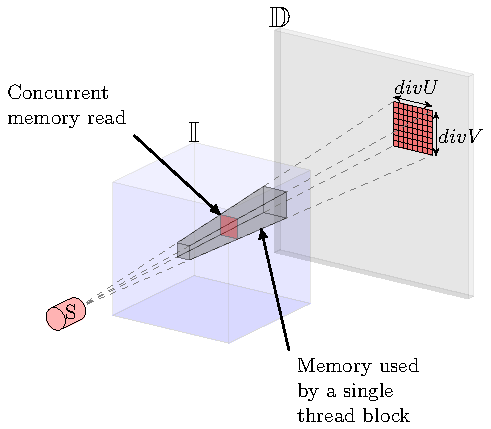
\includegraphics{GPUmethods/threadblocks-figure0.pdf} 
\end{center}

\caption[Diagram of trheadblock optimized kernel execution]{\label{fig:block} Diagram of the block level execution and memory access to increase data locality. Each block is composed of $divU\times divV$ rays, which are executed in parallel. This ensures that the concurrent memory reads are spatially adjacent, thus decreasing memory latency.} 
\end{figure}




\subsection{Grid-interpolated methods}

The grid-interpolated method is significantly less complex than the ray-voxel intersection method. As shown in figure \ref{fig:AmatrixInterp}, it merely relies on sampling the X-ray paths with a uniform Euclidean sampling distance. It can be described using equation \ref{eq:interpolated} and its pseudocode is given in \ref{alg:gridinterp}.

\begin{equation}
d_{(uv)}= \sum_{\alpha}\Delta l*\mathbb{I}(p_x(\alpha),p_y(\alpha),p_z(\alpha)),
\label{eq:interpolated}
\end{equation}
where $\alpha$ is the parameter of the line equation and takes decimal values between 0-1 if defined in terms of the source and detector locations (see equation \ref{eq:line}). Note that now the image $\mathbb{I}$ is sampled using not integer values, but decimal values, thus requiring interpolation. The texture memory cache includes hardware accelerated linear interpolation, so this is interpolation method used. Whereas in equation \ref{eq:ray-voxel} the length in this projection method, $\Delta l$, is a constant the same for all samples and thus can be taken out of the summation.

\begin{algorithm}

\caption{Grid interpolated projection
\label{alg:gridinterp}}
\begin{algorithmic}[1]
\State{Precompute geometric constants}
\Require{$N_{ray}$ threads organized in divU$\times$divV blocks}
    
\For{X-ray path}
      \State{Compute $[x_p,y_p,z_p]$ sample position}
      %\State{Sample $[\textup{DVF}_x,\textup{DVF}_y,\textup{DVF}_z]= \textup{DVF}(x,y,z)$}
      \State{Sum+= $ \textup{Image}(x_p,y_p,z_p)$}      
\EndFor
\State{Detector($u,v$)=$\Delta l \cdot Sum$}
\Ensure{} 
\end{algorithmic}

\end{algorithm}


The memory latency is significantly decreased by choosing the same structure for block and thread organizing as used in the other method and shown in figure \ref{fig:block}. The sampling rate of $\alpha$ is the relevant parameter to set and, as discussed by Jia \textit{et al}\cite{jia2012gpu}, it defaults to half the voxel size to ensure all data are used. The implementation in TIGRE additionally blocks the user from choosing a sampling rate larger than a voxel by limiting it to that size and changing the interpolation to nearest neighbour.

This method of projection is arguably more realistic than the ray-voxel projection in the case where the voxel size is very big (the resolution is very low) as it treats image information as a continuous domain instead of square boxes.

\subsection{Comments on optimization}

In order to minimize the computation times several optimization tricks have been used in both projection types. As one of the challenges of GPU programming is that often the only way of knowing how to accelerate code or what approach to use is intuition and testing, describing the optimization tricks and tests used for acceleration can be important. Three tricks that are worth mentioning are implemented, namely choosing an optimal coordinate system, precomputing geometric unit changes, and the way out of bounds memory is handled. Aside from these, other small tweaks can be found in the code, such as never computing trigonometric functions inside the kernels, but they are all relatively trivial and no further comment on them will be made.

\subsubsection{Optimal coordinate system}

When designing a kernel one of the main considerations is to minimize the amount of arithmetic operations happening inside. In tomography specifically, the geometry is the most variable of the parameters. Images can be arbitrarily fine or coarse and voxels can be anisotropic with a wide range of sizes in each direction and so can the detector. Thus, when writing the kernel, a coordinate system is needed that can accommodate the flexibility of the geometry while still being minimal in arithmetic operations. In TIGRE, the following has been chosen for the projector operator.

As the image memory is static, and data needs to be sampled from it in the projection coordinate system, the image will never move, while the detector and the source will rotate around the axis of rotation. Thus the new system ($x_p,y_p,z_p)$ is aligned with the image edges and it is centred at the first lexicographically indexed voxel, at the bottom corner of the image as seen in figure \ref{fig:projcoord}.  Additionally, the units of the new system are set as voxels, regardless of the size of the voxels in each direction. This new system reduces the amount of arithmetic operations as each sample point is now an index in the image memory, while in each kernel the vector from the source to the detector position must be computed arithmetically. Thus, in the main loop where the new sample location is needed, once the next point in the line is computed no more operations are needed to convert to memory index. This alone saves a significant time.


\subsubsection{Precomputation of geometry}

In order to generate the new coordinate system, some transformations need to be applied to the input geometry, as the units, source location and detector locations need to be set up. All these operations are performed outside the kernel and output 2 points and 2 vectors. The points are the location of the source and first detector pixel with respect to the new coordinate system origin, rotation angle and other geometric definitions. The vectors describe the unit change in projection coordinate systems of the detector pixel location, thus by knowing the location of the first detector pixel and their unit changes, finding any detector pixel location from its index is trivial.

Additionally, the advantage of structuring the geometry computations as described is that new geometric transformations can be implemented with zero increase in computational cost. For example, the addition of the rotation with 3 degrees of freedom of the detector, offset of the image with respect to the axis of rotation or offset of the detector implies no change in computational cost, the only change needed is the change in the 2 points and vectors described.
 
 % sampling outside the image
\subsubsection{Sampling outside the image}

In the ray-voxel method, sampling outside the image is not a worry as the amount of cross-sections and the initial intersection are computed in the algorithm. However, in the grid-interpolated method, a start and end point for sampling need to be chosen. 

As the texture memory is cached and handled differently than a direct read into memory, it has multiple tunable features. One of these is the possibility of selecting the behaviour when a memory read is out of bounds, which in the case of this work is set to zero. It is important to note that this means the code will not generate an error for out of bounds memory reads. Two versions of the grid-interpolated method can be tested, one where there is a conditional check to see if the current point is inside the image and if true then sample, and another where the line is sampled from the source to the detector. Empirical tests show that avoiding the conditional statement and sampling over the whole path is 33\% faster than checking if the sample is within bounds, even with geometry definitions where more than 50\% of the samples lie outside the image. This can be explained by the fact that CUDA cores are quite slow with code control flow and possibly\footnote{This is undocumented so, while it is very likely, it is hard to claim with full certainty.} by the cache taking virtually no time returning a zero value when accessed out of bounds. 

% explain min max radius for out of bounds
Sampling the x-ray path from the start to the end is not optimal either, even avoiding conditional statements. To minimize the memory reads, the diameter of a cylinder that encloses the image is precomputed and the rays are sampled from the beginning of the cylinder to either the detector or to the end of the cylinder, whichever comes first. This approach speeds the projection kernel by another 20\%. This is shown in figure \ref{fig:projcoord}.

\begin{figure}
\begin{center}

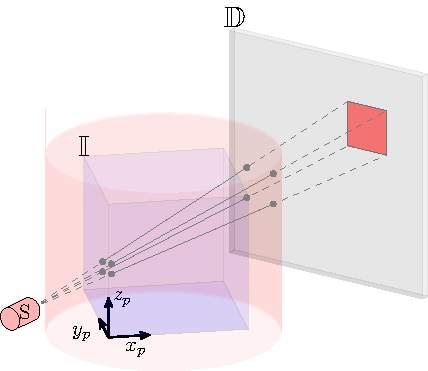
\includegraphics{GPUmethods/projcoord-figure0.pdf} 
\end{center}

\caption[Projection coordinate system]{\label{fig:projcoord} Diagram of the projection coordinate system and sampling region. In both projection operations the new coordinate system ($(x_p,y_p,z_p)$) has its origin on the lexicographically first voxel center. The red cylinder shows the sampling region for the grid-interpolated method, where the kernels sample from memory.} 
\end{figure}
\subsection{Differences between operators}

The projection operators, while effectively simulating the same physics, have slightly different results due to the methods used. The difference between the two projection operators is enhanced when the voxel size of the images is very big, i.e., when the image has low resolution. Figure \ref{fig:projtypes} shows this effect. A projection of the 3D Shepp-Logan phantom is shown at different resolutions for both projection types. In the figure, four image resolutions can be seen for the same size, $64^3$, $128^3$, $256^3$ and $512^3$ from top to bottom. From left to right the first two columns show the ray-voxel intersection and the grid-interpolated method, while the last two columns show a zoomed in version of the same projections. Figure \ref{fig:projtypesdiff} shows the differences between the projections.

The ray-voxel intersection method does introduce higher aliasing-like artefacts to the projection, as opposed to the interpolating method that smooths everything. Note however that when the image resolution gets higher, the differences are almost indistinguishable. None of the projection modes is better or worse. One could argue that the ray-voxel method aligns better with the discretization of the domain, or that the interpolated method is better because it generates images that are closer to what is measured in a real detector. 


When used in reconstruction, the differences between the images reconstructed with algorithms using one or the other projection types are insignificant, with generally a maximum value of about 0.1\% of the highest value in the image. This can be seen in figure \ref{fig:OSSART200proj}, where a reconstruction of the XCAT\cite{XCAT} phantom of size $256^3$ using OS-SART with 200 iterations and 100 projections is shown. It shows the result using both projection operators, and figure \ref{fig:OSSART200projdiff} the contrast enhanced differences (the colourmap is enhanced to 10\% of the maximum data value) of both reconstructions against the original image. Both reconstructed images are visually very similar and the enhanced difference images show structural differences in the error, but they are still of the same level. The sum of square errors shows a slight higher value for the ray-voxel method, but not big enough to be significant. This difference is even smaller when working with higher resolution images. TIGRE defaults to the interpolated projection in the algorithms.

% RMSE= 3.18 vs 2.73


\begin{figure}
\centering
\begin{tikzpicture}

\node (A) {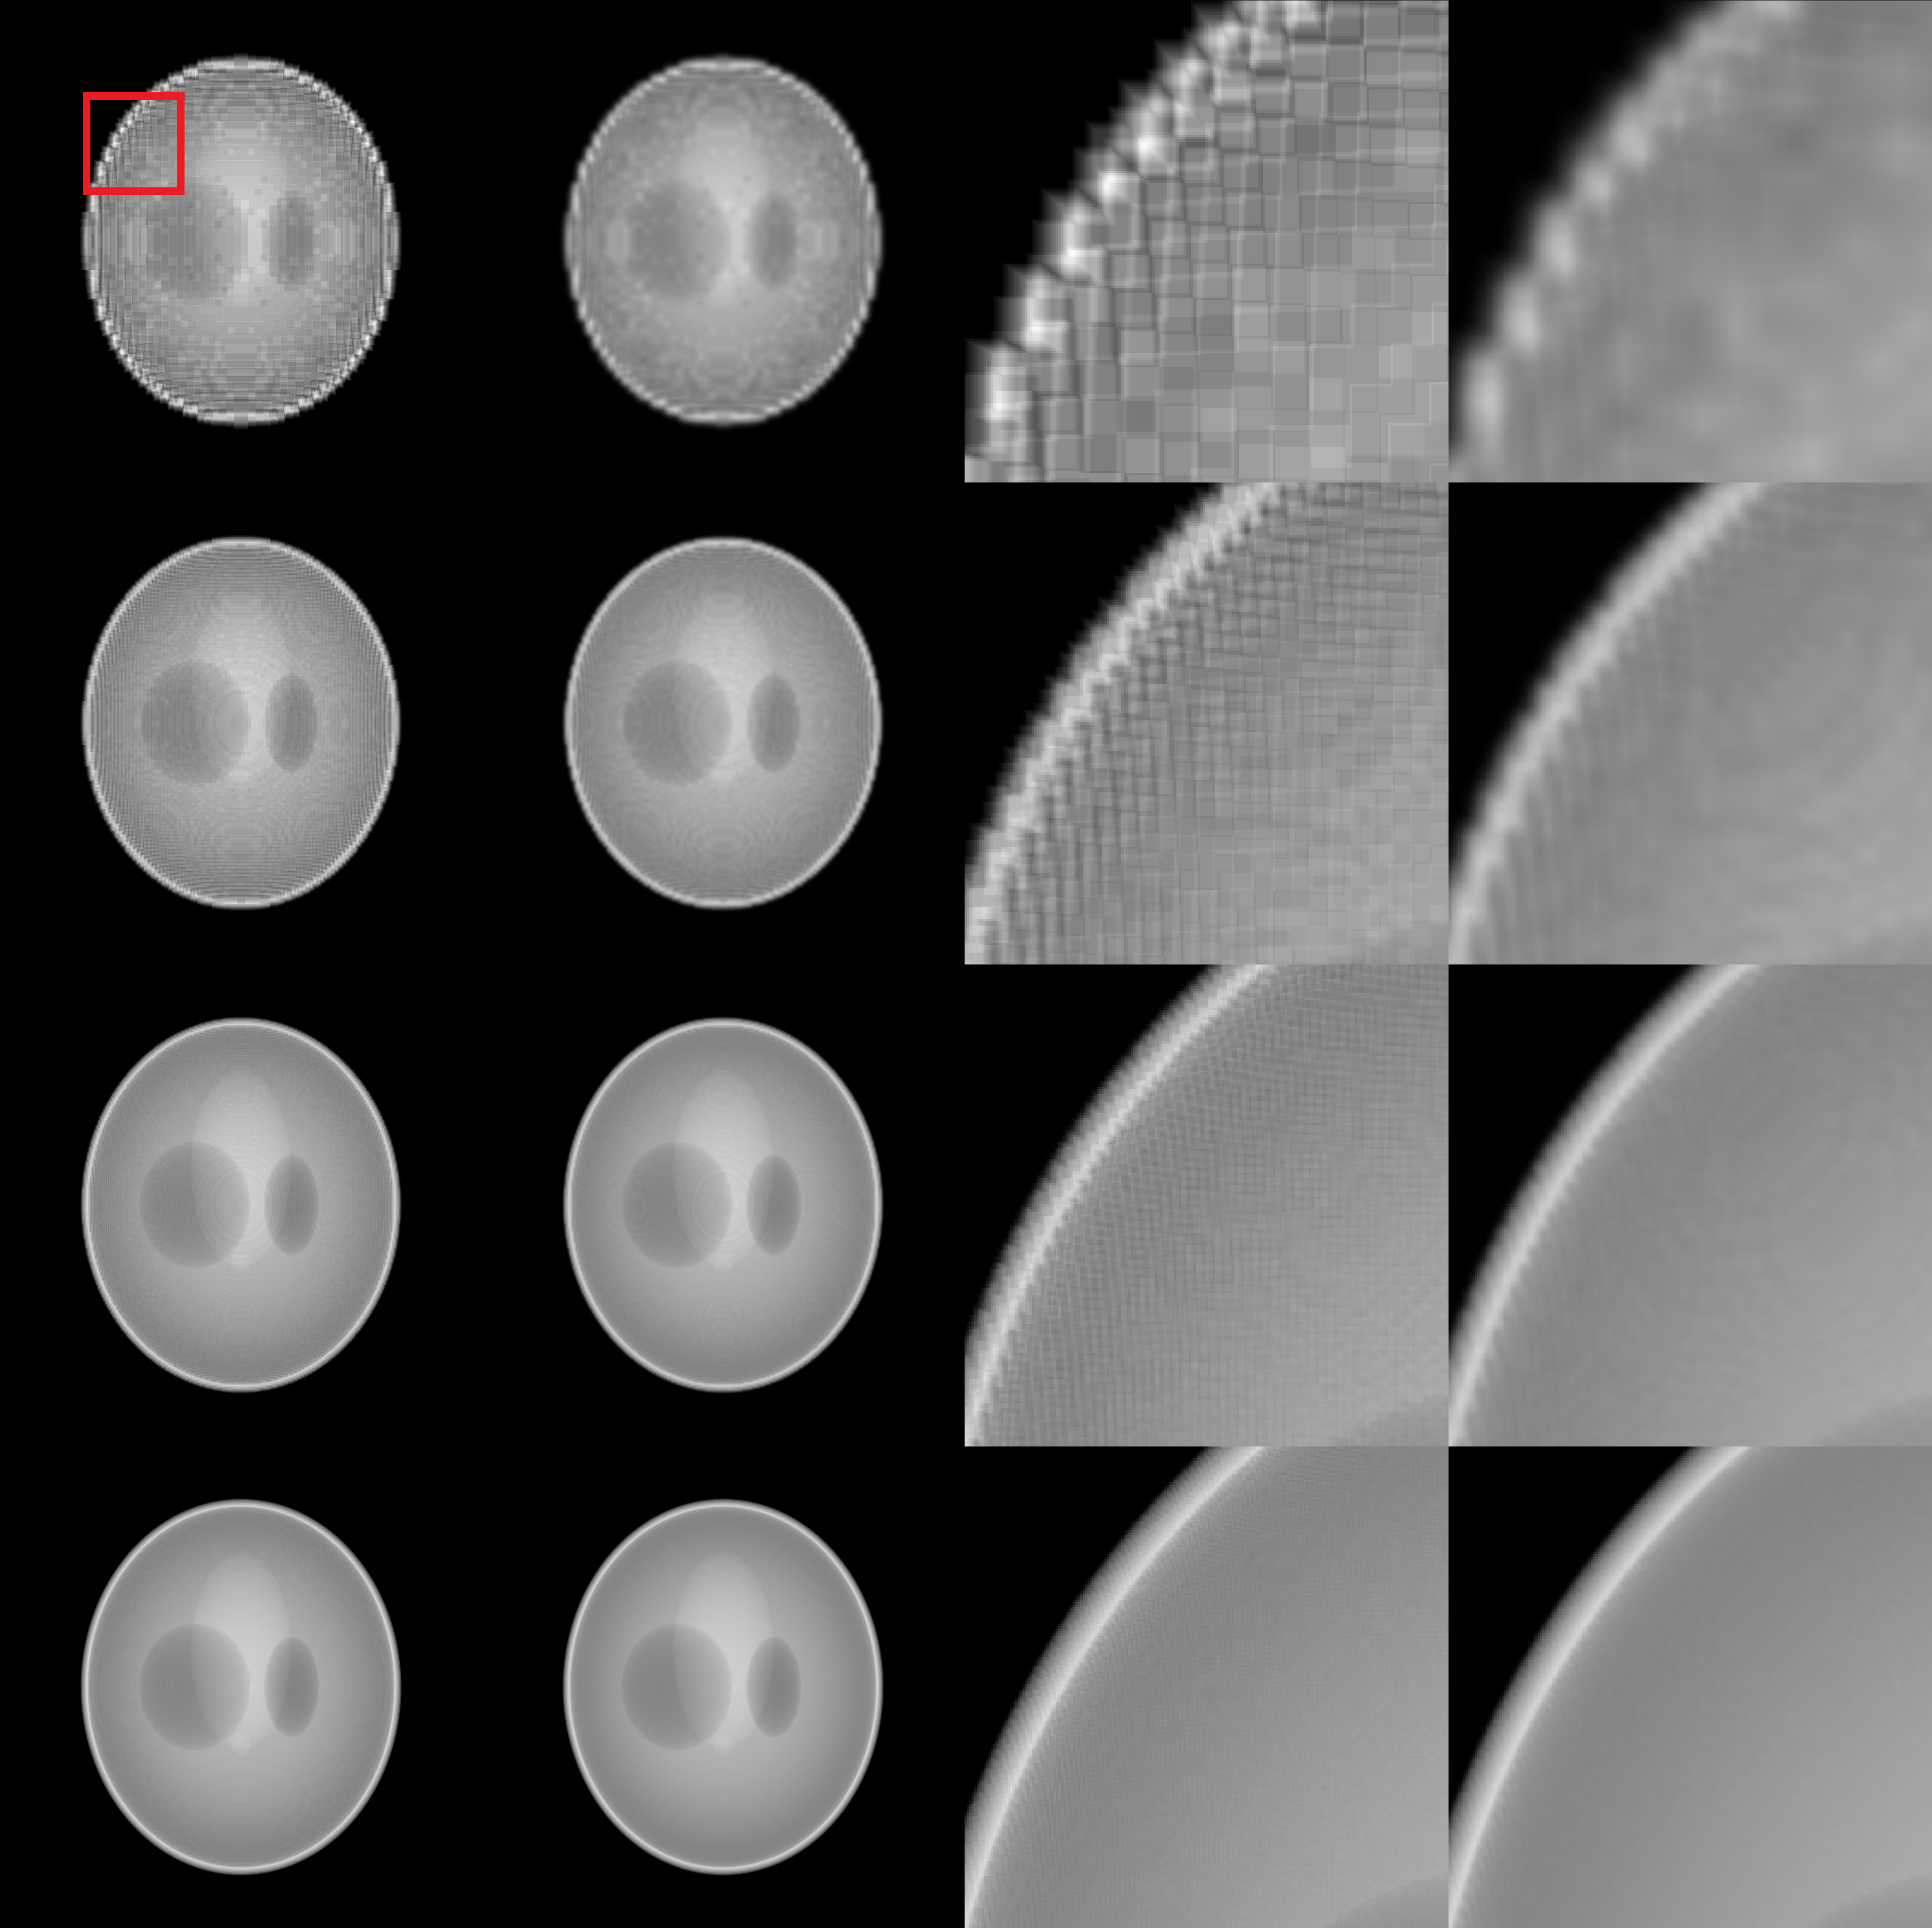
\includegraphics[width=0.94\textwidth]{GPUmethods/projtypes.png} };
\path (A.south west) -- (A.north west) node[pos=.125, above, rotate=90] {$512^3$} node[pos=.375, above, rotate=90] {$256^3$} node[pos=.625, above, rotate=90] {$128^3$} node[pos=.875, above, rotate=90] {$64^3$};
\path (A.south west) -- (A.south east) node[pos=.125, below] {(a)} node[pos=.375, below] {(b)} node[pos=.625, below] {(c)} node[pos=.875, below] {(d)};

\end{tikzpicture}

\caption[Comparison between projection operations]{\label{fig:projtypes} Different projection modes for different image resolutions. From top to bottom, the image resolution is $64^3$, $128^3$, $256^3$ and $512^3$ respectively. From left to right, (a) the ray-voxel intersection projection; (b) the grid-interpolated projection; (c) a zoomed in version of (a); and (d) a zoomed in version of (b).} 
\end{figure}

\begin{figure}

\centering
\begin{tikzpicture}

\node (A) {\includegraphics[width=0.94\textwidth]{GPUmethods/projtypesdiff.png} };
\path (A.south west) -- (A.north west) node[pos=.125, above, rotate=90] {$512^3$} node[pos=.375, above, rotate=90] {$256^3$} node[pos=.625, above, rotate=90] {$128^3$} node[pos=.875, above, rotate=90] {$64^3$};
\path (A.south west) -- (A.south east) node[pos=.125, below] {(a)} node[pos=.375, below] {(b)} node[pos=.625, below] {(c)} node[pos=.875, below] {(d)};

\end{tikzpicture}
\caption[Difference between projection operations]{\label{fig:projtypesdiff} Difference between projection modes for different image resolutions. From top to bottom, the image resolution is $64^3$, $128^3$, $256^3$ and $512^3$ respectively. From left to right, (a) the absolute difference between the projections; (b) contrast enhanced version of (a) by cropping the colourmap to 25\% of the maximum; (c) a zoomed in version of (a); and (d) a zoomed in version of (b).} 
\end{figure}


\begin{figure}
\centering
\begin{tikzpicture}

\node (A) {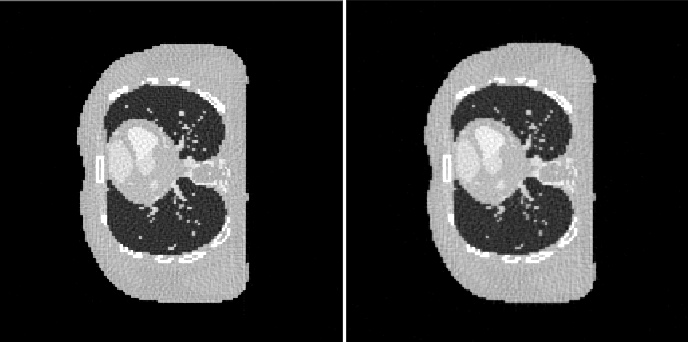
\includegraphics[width=0.98\textwidth]{GPUmethods/OSSART200.png} };
\path (A.south west) -- (A.south east) node[pos=.25, below] {(a)} node[pos=.75, below] {(b)};
\end{tikzpicture}

\caption[Reconstruction example using different projection operators]{\label{fig:OSSART200proj} XCAT phantom reconstruction of size $256^3$ using OS-SART with 200 iterations and 100 angularly uniformly sampled projections. (a) Reconstruction using ray-voxel intersection projection and (b) using the interpolated-projection method.} 
\end{figure}


\begin{figure}
\centering
\begin{tikzpicture}

\node (A) {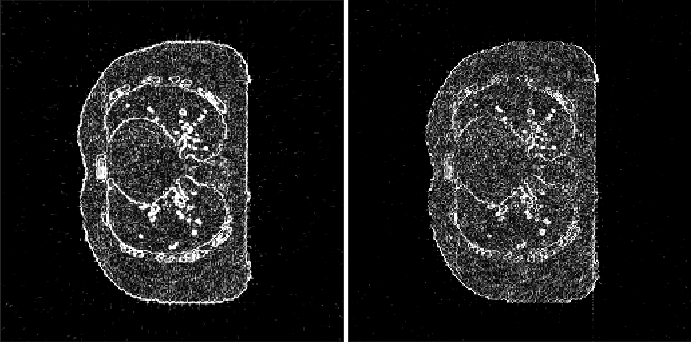
\includegraphics[width=0.98\textwidth]{GPUmethods/OSSART200diff.png} };
\path (A.south west) -- (A.south east) node[pos=.25, below] {(a)} node[pos=.75, below] {(b)};
\end{tikzpicture}

\caption[Difference in reconstruction using different projection operators]{\label{fig:OSSART200projdiff} Difference between the original XCAT phantom and the reconstructions of figure \ref{fig:OSSART200proj}. The colour limits have been set to 10\% of the maximum intensity of the original data.  (a) Difference using ray-voxel intersection projection and (b) difference with the interpolated projection method.} 
\end{figure}



\FloatBarrier

\section{The backprojection operator}

The backprojection operator (or $A^T*b$ in algebraic notation) is the operator that updates the image using the information in the projection images. This update is performed by an operation often described in the literature as a smearing of the projection data into the image, as if it were butter on toast, but following the path from detector to source.

As with projection, multiple methods to perform this operation have been proposed in the literature. The most commonly used method is voxel-driven backprojection\cite{scherl2007fast}\cite{okitsu2010high}, where the path from the source to each voxel center is generated and extended until the detector is reached. Then the value in the detector is sampled (using interpolation, as it is likely that it does not fall in the center of a pixel) and the voxel value updated.
 
Other methods include the separable footprints method\cite{long20103d}, where the footprint of the voxel in the detector is precomputed and approximated and the voxel values are updated according to the detector values overlapping the voxel footprint. A conceptually similar backprojection relies on having spherical shaped image value representation, instead of square voxels\cite{spherical}. The backprojection using basis-functions also updates the image values according to the footprint of these spherical voxels.
 
The distance-driven method\cite{schlifske2016fast} is also applicable to backprojection by performing the same operation as for projection: the computation of all voxel-pixel intersections in an imaginary mid-plane. Finally, ray-voxel intersection driven methods also exist\cite{park2015fully}, in both single ray or multiple ray per voxel modes. This method requires multiple voxel updates per backprojection, but can give a matched result, i.e., the backprojection method is the same as the projection method. This has been shown to give better results\cite{6829349} and allows the use of any iterative method Krylov subspace methods require matched backprojection. 
 
In this work, voxel-driven backprojection has been implemented. The rationale being that it is a method which is fast and easy to implement yet accurate. Additionally, a quasi-matched backprojection can be implemented to allow Krylov subspace algorithms (see section \ref{sec:weights} for more information). Finally, this method is most appropriate for the method proposed in Chapter 6.
 

\subsection{Voxel-driven backprojection}

The underlying idea of voxel-driven backprojection is simple, the path between the source and the center of each voxel is computed and the intersection of that path with the detector is computed. Then, the detector is sampled at the intersection point (using interpolation) and the voxel is updated with that value. Due to the cone angle, a weighting factor is also applied to each voxel (more details are given in the next section).

\begin{figure}
\begin{center}

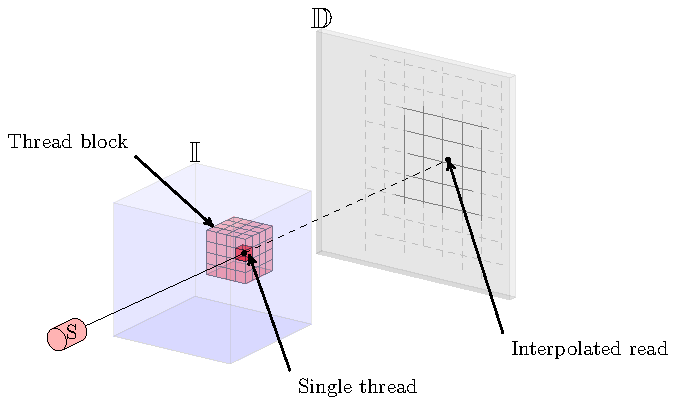
\includegraphics{GPUmethods/simplebackproj-figure0.pdf} 
\end{center}

\caption[Diagram of the voxel driven backproejction]{\label{fig:simpleback} Simple voxel-driven backprojection. Each kernel is subdivided into square blocks and each thread updates a single voxel using interpolated memory reads in the detector.} 
\end{figure}


To accelerate this operator in a GPU, the naive approach is to assign a thread per voxel and to assign a square amount of threads to a single block (by dividing it into divX$\times$divY$\times$divZ threads) to maximize cache hits on texture memory (used for the interpolation of the detector values). The block size is empirically set to 8x8x8 for fastest execution. This approach, shown as a diagran in figure \ref{fig:simpleback} and as pseudocode in algorithm \ref{alg:naiveback}, does indeed result in a fast kernel. However, the backprojection requires a significantly higher total number of threads than the projection operation, while repeating the same thing for each voxel (in multiple bakcprojection updates) and reading in the same memory very often. In order to improve the cache memory hits and minimize redundant arithmetic computations, a series of improvements have been studied by Papenhausen \emph{et al}\cite{papenhausen2011gpu} and further optimized by Zinsser \emph{et al} \cite{zinsser2013systematic}.

\begin{algorithm}

\caption{Naive voxel-driven backprojection
\label{alg:naiveback}}
\begin{algorithmic}[1]
\For{Projection}
\State{Precompute geometric constants}


\Require{$N_{voxel}$ threads organized in divX$\times$divY$\times$divZ blocks}
      \State{\qquad Compute $[u,v]$ sample position}
      %\State{Sample $[\textup{DVF}_x,\textup{DVF}_y,\textup{DVF}_z]= \textup{DVF}(x,y,z)$}
      \State{\qquad Compute $w$ weight}
\State{\qquad Image($x,y,z$)+=$w  \cdot \textup{Detector}(u,v)$}
\Ensure{} 
\EndFor

\end{algorithmic}

\end{algorithm}


The main idea behind the optimization is the minimization of memory latency. In order to do that a multiple voxel, multiple projection per thread kernel is designed. If in each of the threads when a single voxel is updated multiple projections (32 in this case) are used, these will be spatially nearby, thus the L2 cache will speed up the memory reading process provided the angular distance between projections is small. Additionally, if each of the threads computes a small subset of voxels ($N_{voxelThread}$) in the $z$ direction (8 in this case), not only are the memory cache hits are likely to be increased, but also the computational operations reduced as the computation of the location of each voxel requires fewer operations. In general these tweaks increase the occupancy of the SMs, decreasing the amount of time the threads stand idle waiting for memory. The diagram of the new optimized kernel is shown in figure \ref{fig:optback} and its pseudocode is given in algorithm \ref{alg:optimizedback}. The code is divided in pieces to allow each block to have divX$\times$divY threads each (16$\times$32 in this case). To minimize global memory reads, the image voxel values that are updated in each kernel are pre-loaded. Then, for each projection, the geometric constants that describe the location of the detector and image pixels are loaded from constant memory. Next, the backprojection is performed for each voxel being updated. This approach further increases occupancy as in execution the thread does not wait for the memory read to finish before computing the next loop, thus hiding memory latency even more. Finally, the image is updated with the auxiliary variable. This step also decreases the memory latency, as fewer global memory write operations are needed.
% describe better the algorithm


\begin{algorithm}

\caption{Optimized voxel-driven backprojection
\label{alg:optimizedback}}
\begin{algorithmic}[1]
\For{$N_{kernels}$}
\State{Precompute geometric constants \textit{per projection}}

\Require{divX$\times$divY threads organized in $\frac{N_x}{\textup{divX}} \times \frac{N_y}{\textup{divY}} \times \frac{Nz}{N_{voxelThread}}$ blocks}
\For{$N_{voxelThread}$}
\State auxImage(voxThread)=Image($x,y,z$)
\EndFor  
\For{Projections (in this kernel)}
\State{Load geometric constants for this projection}
\For{$N_{voxThread}$}
\State{Compute $[u,v]$ sample position}
\State{Compute $w$ weight}
\State{auxImage(voxThread)+=$w  \cdot \textup{Detector}(u,v)$}
\EndFor
\EndFor
\For{$N_{voxThread}$}
\State{Image($x,y,z$)=auxImage(voxThread)}
\EndFor
\Ensure{} 
\EndFor

\end{algorithmic}

\end{algorithm}
\begin{figure}
\begin{center}

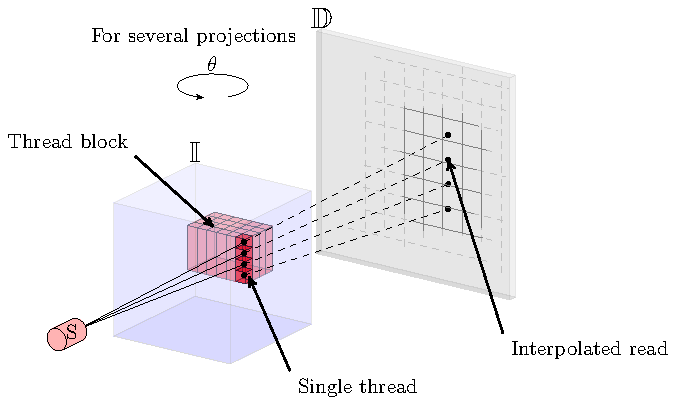
\includegraphics{GPUmethods/optbackproj-figure0.pdf} 
\end{center}

\caption[Diagram of multiple-voxel, multilpe-angle backprojection]{\label{fig:optback} Optimized voxel-driven backprojection. Each kernel is subdivided into blocks and each thread updates a series of vertical voxels using interpolated memory. Each kernel additionally operates in a series of projections, not in a single one.} 
\end{figure}

\subsection{Backprojection weights}\label{sec:weights}

Due to the cone shape the backprojection needs a weight for each voxel, as different paths have different ray lengths and hence have a different effect in the detector. In the projection operator, the length of the path is used in each detector pixel as a weight for the update, but in the backprojection operation the weight is not as straightforward to compute. In the algebraic definition of iterative algorithms, the weight of each voxel is the length of a specific ray within that voxel. If the matrices were fully known, it would be straightforward to compute (as it is the sum of the columns of $A$), however this doesn't apply to voxel-driven backprojection. In the GPU version, a projection to compute such lengths per backprojection would be needed, ultimately slowing the code considerably.

\subsubsection*{FDK weights}
A simple approach is to use the weights of the FDK algorithm as backprojection weights. As described in section XX, the FDK backprojection weight is computed as

\begin{equation}
w_{x,y}=\frac{R^2}{(R+y\cdot \sin\theta-x\cdot\cos\theta)^2},
\end{equation}
where $R$ is the distance from the source to the axis of rotation, $\theta$ the projection angle and $x$ and $y$ the location of the voxel. Note how this equation is independent of $z$, thus the weights can be precomputed after line 7 (instead of line 10) in algorithm \ref{alg:optimizedback}, resulting in a minor speed-up.


\subsubsection*{Pseudo-matched weights}
The FDK weights are good in the iterative algorithms that normalize the result of the backprojection afterwards (such as SART), as the overall scale and effect of the backprojections is removed in the algorithm by an opposing weighting factor. However, some algorithms require matched backprokection, i.e., a backprojection operator that is mathematically equivalent to the adjoint of the projection operator. This is not the case with FDK weights. Algorithms such as CGLS cannot work unless a matched backprojection is implemented. As previously explained, a fully matched backprojection, while possible, would slow down the kernels considerably due to the need of also computing projection operations in the backprojection. However Jia \textit{et al}\cite{jia2011gpu} propose a weight to match the backprojection.

In order to derive the weight, a functional analysis approach needs to be taken. For the sake of simplicity and cohesion with Jia \textit{et al}, the notation in this section differs from the rest of the thesis. 

If an image is represented as a function $f(\textbf{x})$, where $\textbf{x}=(x,y,z)\in \mathbb{R}^3$, a projection operator $A^\theta$ maps $f(\textbf{x})$ onto a different function on the projection plane with angle $\theta$ as:
\begin{equation}
A^\theta[f](\textbf{u})=\int_0^{L(\textbf{u})}\mathrm{d}l \ f(\textbf{x}_s+\textbf{n}l),
\label{eq:functionalXray}
\end{equation}
where $\textbf{x}_s$ is the coordinate of the source, $\textbf{n}$ a unit vector in the projection direction and $\textbf{u}\in \mathbb{R}^2 $ the coordinates in the detector. $L(\textbf{u})$ is the length of the X-ray path. 

Let $f(.):\mathbb{R}^3 \rightarrow \mathbb{R}$ and $g(.):\mathbb{R}^2 \rightarrow \mathbb{R}$ be smooth enough functions in image and  projection domain respectively. In order to to have an operator $A^{\theta^T}$ that is the adjoint of $A^\theta$, it should satisfy the condition 

\begin{equation}
\langle f, A^{\theta^T} g\rangle = \langle A^\theta f,g \rangle,
\end{equation}
where $\langle \cdot, \cdot\rangle $ is the inner product. In integral form, this inner product equality can be expressed as
\begin{equation}
\int \mathrm{d}\textbf{x}f(\textbf{x})A^{\theta^T} [g](\textbf{x})=\int \mathrm{d}\textbf{u}A^{\theta} [f](\textbf{u}) g(\textbf{u}),
\end{equation}
or if the functional derivative of both sides with respect to $f(\textbf{x})$ is taken, then as
\begin{equation}
A^{\theta^T} [g](\textbf{x})=\frac{\partial}{\partial f(\textbf{x})}\int \mathrm{d}\textbf{u}A^{\theta} [f](\textbf{u}) g(\textbf{u}).
\label{eq:matchedback3}
\end{equation}
Equation \ref{eq:matchedback3} can be rewritten as
\begin{equation}
A^{\theta^T} [g](\textbf{x})=\int \mathrm{d}\textbf{u}g(\textbf{u})\frac{\partial}{\partial f(\textbf{x})}A^{\theta} [f](\textbf{u}),
\label{eq:matchedback4}
\end{equation}
and equation \ref{eq:functionalXray} can be rewritten as equation \ref{eq:functionalXraydelta} using a delta function.
\begin{equation}
A^\theta[f](\textbf{u})=\int\mathrm{d}l\mathrm{d}\textbf{x} \ f(\textbf{x})\delta(\textbf{x}-\textbf{x}_s-\textbf{n}l).
\label{eq:functionalXraydelta}
\end{equation}

Finally, by substituting equation \ref{eq:functionalXraydelta} in \ref{eq:matchedback4}, the adjoint of the projection operator can be expressed as

\begin{equation}
A^{\theta^T}[g](\textbf{x})=\int\mathrm{d}l\mathrm{d}\textbf{u} \ g(\textbf{u})\delta(\textbf{x}-\textbf{x}_s-\textbf{n}l)=\frac{L^3(\textbf{u}^*)}{L_0l^2(\textbf{x})}g(\textbf{u}^*),
\end{equation}
where $\textbf{u}^*$ is the intersection point between the x-ray path and the detector plane, $l(\textbf{x})$ the distance between the source and a voxel, and $L_0$ the source to detector distance. This equation, however, applies to the integral form of the description of the system, while ultimately in the computer the matrix form is used. By changing the inner product to a vector form, the final adjoint over all projections becomes
\begin{equation}
A^{\theta^T}[g](\textbf{x})=\frac{\Delta x \Delta y \Delta z}{\Delta u \Delta v}\sum_\theta\frac{L^3(\textbf{u}^*)}{L_0l^2(\textbf{x})}g^\theta(\textbf{u}^*),\label{eq:finalmatched}
\end{equation}
where $(\Delta x,\Delta y,\Delta z)$ are the sizes of each voxel in each direction and $(\Delta u,\Delta v)$ the sizes of the detector pixels. 

This backprojector weight is very close to a matched backprojection operator. According to Jia \textit{et al} the numerical errors are less than 1\%. This work did not replicate their results. This mismatch can lead to inaccuracies in Hounsfield units in the final reconstruction and to divergent behaviour in the Krylov subspace algorithms, but only in late iterations.

\subsection{Comments on optimization}

To have a fast execution of the code, as for the projection, a geometry that minimizes the amount of arithmetic operations inside the kernels is proposed. The backprojection coordinate system $(x_b,y_b,z_b)$ is defined to have unit sizes of the detector pixel size in $u,v$ for $y_b$ and $z_b$ respectively, and 1mm in $x_b$. The origin of the system is located in the center of the first lexicographically ordered pixel in the detector and is always aligned to the detector (i.e., the image rotates while the detector-source system stays in the same location).  All precomputing operations performed in the projection geometry are also performed in here.

In the CUDA sense, two extra optimizations have been performed. By defining divX, divY and $N_{voxelThread}$ (from algorithm \ref{alg:optimizedback}) as compilers, an instruction to the CUDA compiler can be passed to unroll all the loops. Loop unrolling refers to replacing a for loop by a repetition of each line of code per iteration, one after the other. By doing this, the kernel does not need to have flow control (loop iteration, condition, variable) that needs increasing and checking, thus increasing the total kernel performance by 20\% in our case. A small speed-up is also obtained by defining the texture memory as layered memory, thus disabling interpolation in the third dimension.


\FloatBarrier
\section{Benchmark}\label{sec:speed}

This section shows the computational times for the projection and backprojection kernels. This section does test the performance of the kernels themselves, but the actual calls to the kernels do have some overhead of memory input and output, as it is a significant amount of memory that needs to be moved in every call. All computational time results show time per projection, for different image and projection sizes. Figure \ref{fig:projectiontimes} shows the projection times in milliseconds for both ray-voxel intersection and grid interpolated projection modes. The projection operation is dependent in both detector an image size, and it takes about the same time for both types of projection, with  maximum of 100ms with $1024^2$ detector and $1024^3$ image.


 Figure \ref{fig:backprojectiontimes} shows the backprojection times for FDK weights and pseudo-matched weights. As the kernels are optimized for adjacent projection calls the computational times do not scale with more projections, a test using the maximum projections per kernel is also performed. Figure \ref{fig:backprojection32times} shows kernel times per projection when multiple projections are updated. The maximum computational time on these tests ($1024^2$ detector with $1024^3$ image) show 75ms and 180ms for the FDK and pseudo-matched weights when a single projection is used, but 45ms and 99ms per projection when 32 projections (maximum simultaneously used projections in a single kernel) are used. Note that generally the pseudo-matched weights are slower. This is explained by the fact that the chosen kernel structure completely masks the memory latency with FDK weights, but with matched weights the arithmetic operations for the weight need both more computations and registers, thus slowing down the kernel significantly. Additionally an extra multiplication kernel is needed for the final normalization from equation \ref{eq:finalmatched}. Note also how the backprojection times are not dependant on the projection size, only in the image size. This is not a big surprise, considering how the kernels are designed.
 
 

 \color{black}{}
\begin{figure}
\centering
\begin{tikzpicture}
\node (A) {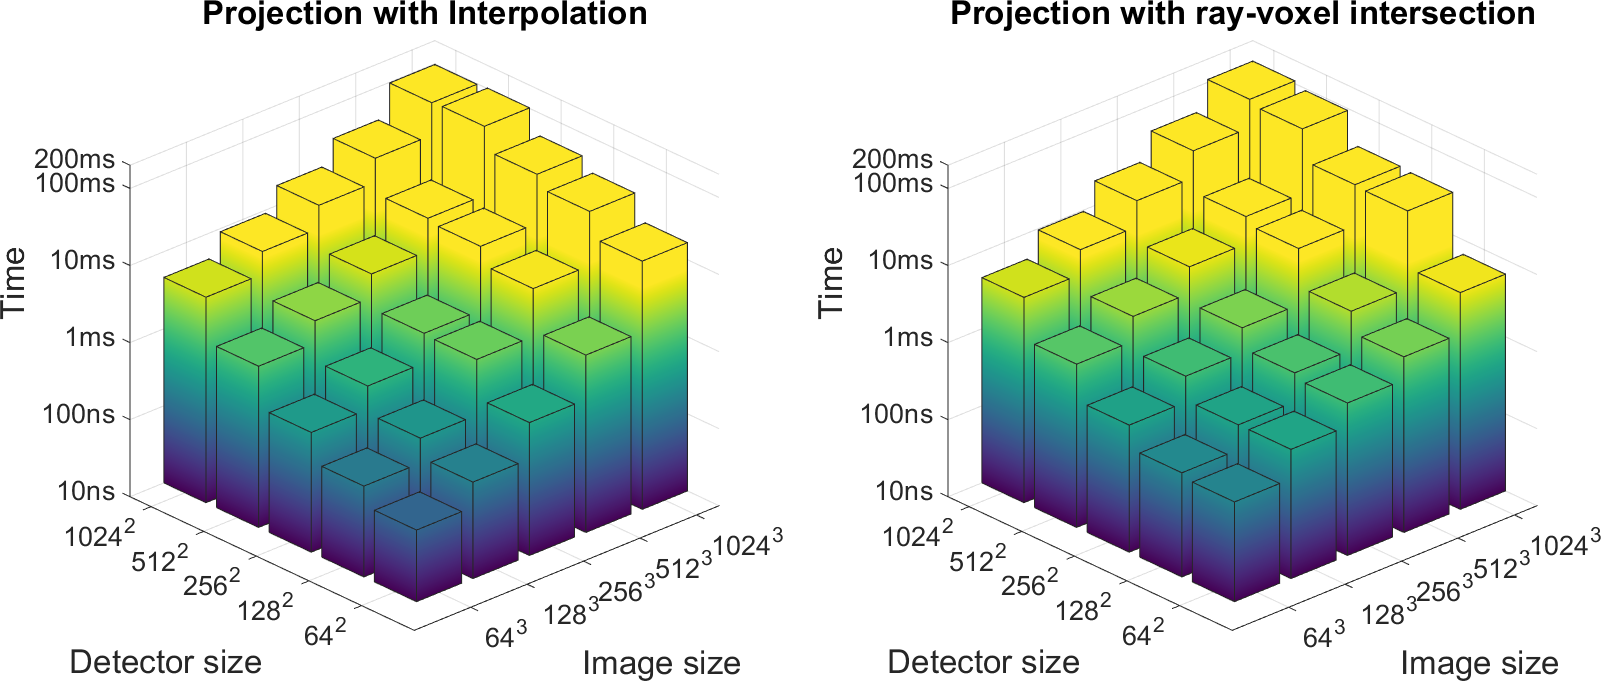
\includegraphics[width=0.98\textwidth]{GPUmethods/projection.png}};
\path (A.south west) -- (A.south east) node[pos=.25, below] {(a)} node[pos=.75, below] {(b)};
\end{tikzpicture}

\caption[Computational times of the projection operators]{\label{fig:projectiontimes} Computational times per projection for the projection operation for (a) grid interpolated (2 samples per voxel) and (b) ray-voxel intersection modes.} 
\end{figure}


\begin{figure}
\centering
\begin{tikzpicture}
\node (A) {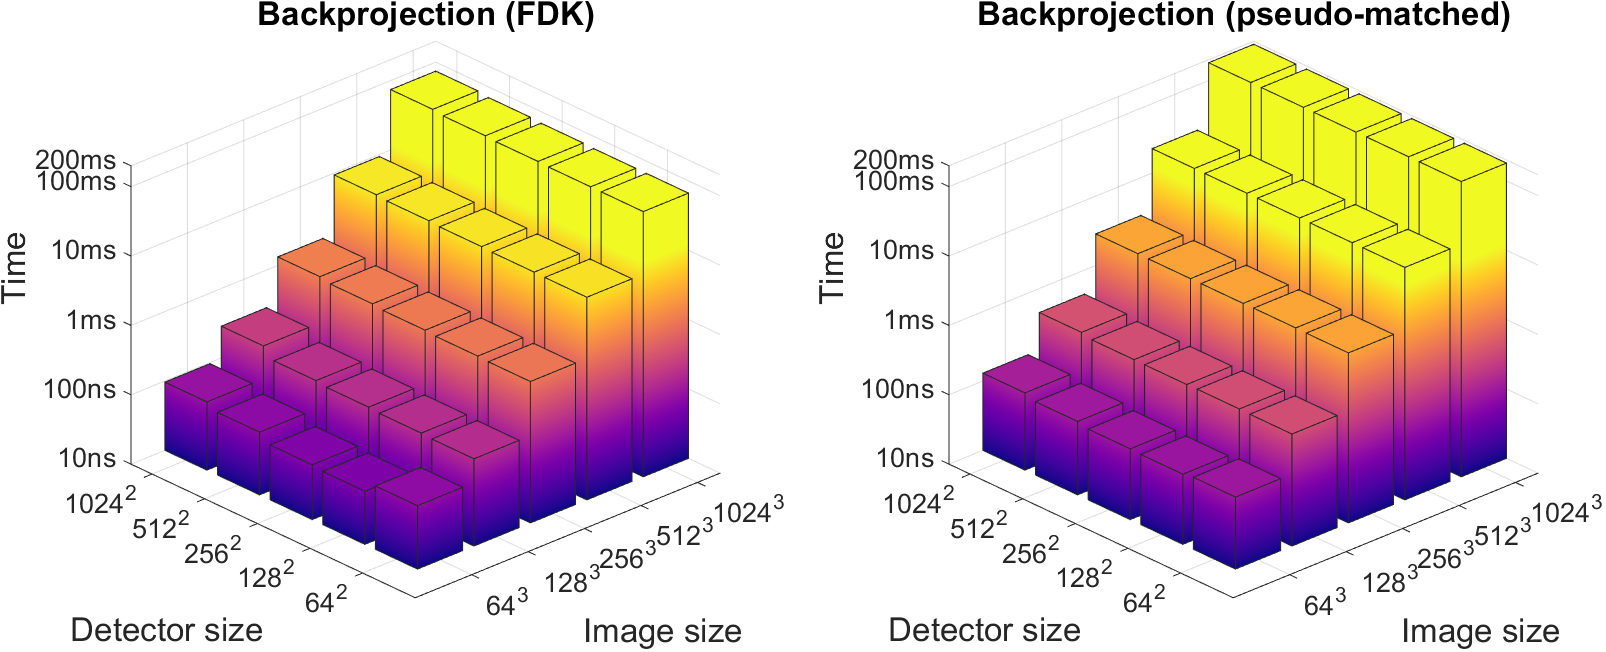
\includegraphics[width=0.98\textwidth]{GPUmethods/backprojection.png}};
\path (A.south west) -- (A.south east) node[pos=.25, below] {(a)} node[pos=.75, below] {(b)};
\end{tikzpicture}

\caption[Computational times of the backprojection operator, per projection]{\label{fig:backprojectiontimes} Computational times per projection for the backprojection operation when launched with a single projections for (a) FDK weights and (b) pseudo-matched weights.} 
\end{figure}

\begin{figure}
\centering
\begin{tikzpicture}
\node (A) {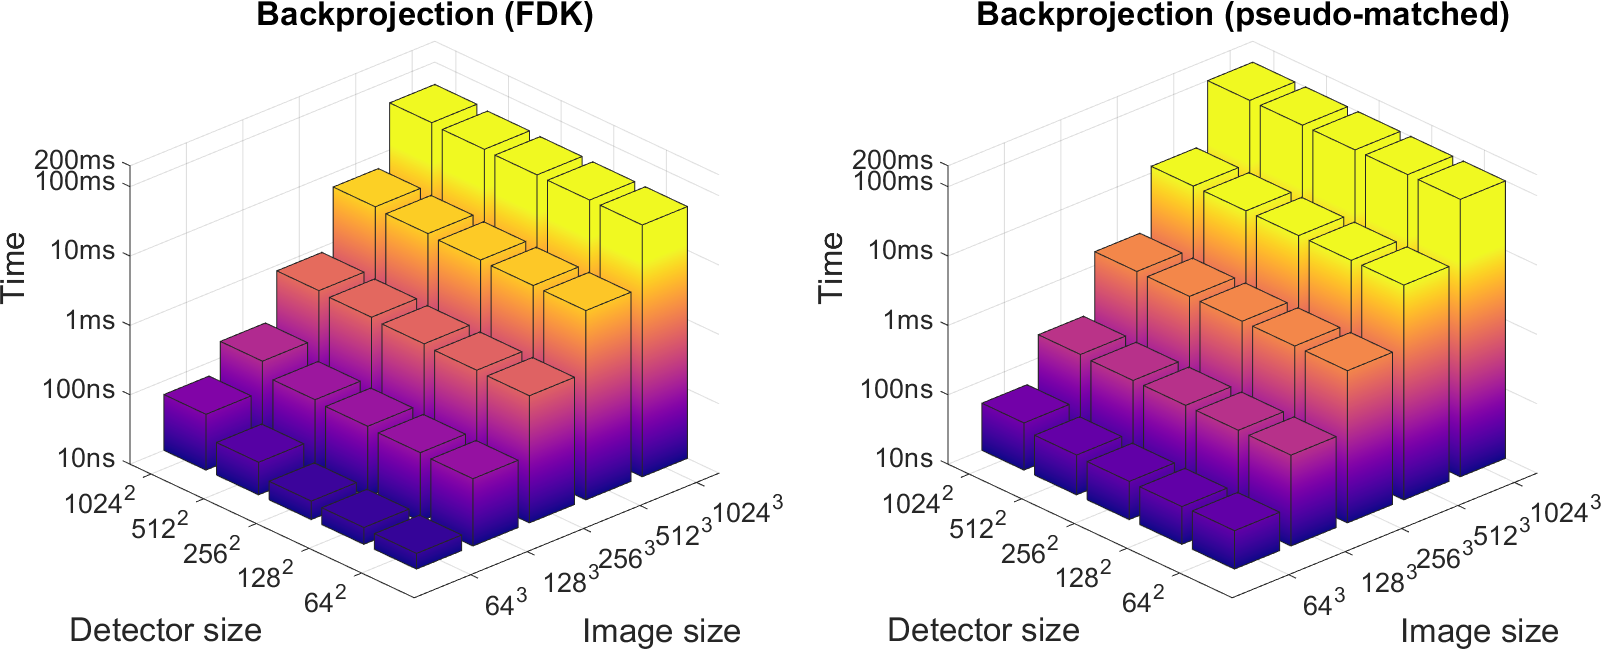
\includegraphics[width=0.98\textwidth]{GPUmethods/backprojection32.png}};
\path (A.south west) -- (A.south east) node[pos=.25, below] {(a)} node[pos=.75, below] {(b)};
\end{tikzpicture}

\caption[Computational times of the backprojection operator, multiple projections]{\label{fig:backprojection32times} Computational times per projection for the backprojection operation when launched with 32 projections for (a) FDK weights and (b) pseudo-matched weights.} 
\end{figure}


\FloatBarrier
\section{The TIGRE toolbox}

In order to have an easy tool to implement algorithms but still have the GPU acceleration on hand, a MATLAB-CUDA toolbox has been created, the Tomographic Iterative GPU-based Reconstruction toolbox, or TIGRE toolbox. TIGRE is a modular, easy to use fast toolbox for cone and parallel beam computed tomography, focusing in the implementation of a variety of iterative reconstruction algorithms. All four families of algorithms described in chapter 3 are implemented in TIGRE, namely, FDK, statistical inversion (MLEM), the gradient descend family (SART,OS-SART,SIRT), Krylov subspace family (CGLS) and TV regularized family (\mbox{ASD-POCS},  \mbox{OS-ASD-POCS}, \mbox{B-ASD-POCS-$\beta$}, SART-TV). This section describes the features of TIGRE, the geometry supported, the general structure of the toolbox and how to implement an algorithm on it. This section is partially based in article \cite{TIGRE}.

\subsection{Geometry in TIGRE}

The geometry of CBCT in TIGRE can be represented as in figure \ref{fig:geometryTIGRE}. An X-ray source, $\text{S}$, is located at distance $\text{DSO}$ from a centre of rotation $\text{O}$, where the origin of a cartesian coordinate system is located. The X-ray source irradiates a cone-shaped region containing the image volume $\mathbb{I}$ and a detector $\mathbb{D}$ measures the intensity of the photons attenuated following the Beer-Lamber law. The image is centred at position $\text{O}'$, which is displaced by $\overrightarrow{V_{orig}}$ from the coordinate system origin. The detector, located at distance $\text{DSD}$ from the source and centred at $\text{D}'$, has an offset of $\overrightarrow{V_{det}}$ from $\text{D}$, which is a point lying in the xy-plane at distance $\text{DSD}-\text{DSO}$ from the origin. A projection coordinate system uv is defined centred at the lower left corner of the detector. During the measurement acquisition, the source and the detector rotate around the z-axis at an angle of $\theta$ from their initial position. Additionally, the detector can rotate on its own center by 3 axis of rotation, useful to account for mechanical errors[CITE]. Finally the center of rotation (COR) offset has also been implemented, a common offset in CT machines where the sample rotates, instead of the detector-source system.

While the diagram shows the geometry for CBCT, TIGRE also supports 3D parallel beam geometry, and by setting the offsets of the image accordingly, helical beam geometries. Additionally, if a correct size of the detector is chosen the geometry can be modified to allow 2D reconstruction, however TIGRE is not designed for 3D geometries, as GPU accelerations in 2D are not essential. Code snippet \ref{cs:geometry} shows the code to define the geometry in TIGRE.

\begin{figure}
\begin{center}

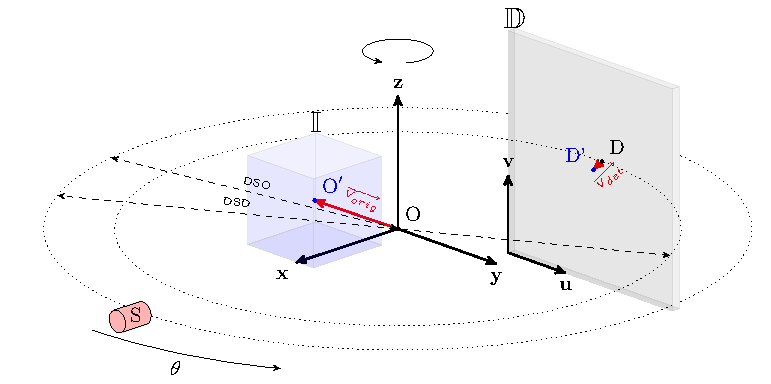
\includegraphics{GPUmethods/geometrytikz-figure0.pdf} 
\end{center}

\caption[Diagram of the geometry of TIGRE]{\label{fig:geometryTIGRE} Diagram of the geometric definition of a TIGRE reconstruction. Image, and detector offsets are supported, as well as any arbitrary size for the image and the detector, both total and pixel-wise.} 
\end{figure}

The geometric variables described above are used in the TIGRE Toolbox to perform the necessary operations for image reconstruction, as shown in code snippet \ref{cs:geometry}. It is worth mentioning that both $\overrightarrow{V_{det}}$, $\overrightarrow{V_{orig}}$, COR and the rotation of the detector are vectors that can be defined per projection angle $\theta$.
\FloatBarrier
\begin{lstlisting}[style=Matlab-editor,
basicstyle=\scriptsize,
caption= Geometry definition in TIGRE,
label={cs:geometry},
frame = single
]
%% Geometry structure definition.
% Distances
geo.DSD = 1536;                      	    % Distance Source Detector
geo.DSO = 1000;                     	    % Distance Source Origin
% Detector parameters
geo.nDetector=[512; 512];		    % number of pixels 
geo.dDetector=[0.8; 0.8]; 		    % size in mm of each pixel
geo.sDetector=geo.nDetector.*geo.dDetector; % total size of the detector in mm
geo.rotDetector=[0;0;0];                    % euler angles of the rotation 
% Image parameters
geo.nVoxel=[512;512;512];                   % number of voxels in the image
geo.sVoxel=[256;256;256];                   % total size of the image in mm
geo.dVoxel=geo.sVoxel./geo.nVoxel;          % size in mm of each voxel
% Offsets
geo.offOrigin  =[0; 0; 0];                  % V_orig
geo.offDetector=[0; 0];                     % V_det
geo.COR=0;                                  % Centre of Rotation offset

\end{lstlisting}

\subsection{Structure}

TIGRE has been designed to be modular, in order to facilitate prototyping with instant acceleration and to allow easy of the toolbox. The main building blocks are the projection ($A(x)$) and back projection ($A^T(b)$) operators. In the TIGRE Toolbox, these two blocks have been optimized for GPU computing using CUDA, as described in the beginning of this chapter. They lie in the lowest layer of the toolbox design and are constantly used by the other layers. The algorithms themselves lie in the topmost layer and are all coded in MATLAB, which provides the power and flexibility of a high-level language. To be able to communicate between the low-level, hardware-oriented CUDA and the high-level, design-oriented MATLAB, a set of the so-called \textit{MEX functions} are needed. The toolbox has been designed not to have any specific data types or classes. Instead, it comprises only the basic MATLAB types, such as matrices and structures.

The high level algorithms are designed to have multiple parameters and full customization. The only required parameters to all algorithms are the data, geometry, angles and number of iterations. Each algorithm has a series of tunable parameters. Generally every parameter affecting the algorithm can be set up to have a different value, allowing users that want to study algorithm behaviour full customization, but having default parameters in case the users want an easy-to use algorithm. Multiple algorithm initialization modes, angle ordering schemes and other features are also available. 

\begin{figure}
\begin{center}

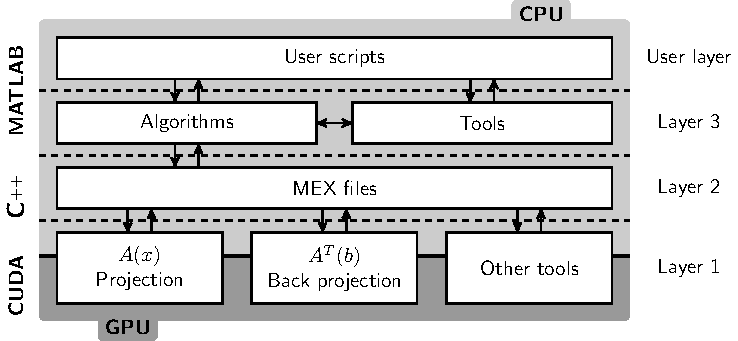
\includegraphics{GPUmethods/structureTIGRE-figure0.pdf} 
\end{center}

\caption[Diagram of the structure of the TIGRE toolbox]{\label{fig:structureTIGRE} Diagram of the structure on TIGRE toolbox.} 
\end{figure}

\subsubsection{Using TIGRE}
This code demonstrates the reconstruction of the RANDO head phantom (data obtained in the Christie Hospital, Manchester, UK) using three different algorithms with the geometry defined in code snippet \ref{cs:geometry}. The data set contains 360 equidistant projections. Once the data have been loaded using the code of snippet \ref{cs:randohead}, the results of figure \ref{fig:RANDOTIGRE} can be obtained without the need for any more code. Information about total computation time and computation time per iteration are shown. Only some of the possible optional parameters to the algorithms are shown in the snippet. The reader is referred to the published documentation for advanced options and for insight into their numerical ranges. 

\begin{lstlisting}[style=Matlab-editor,
basicstyle=\scriptsize,
caption= RANDO head data reconstruction,
label={cs:randohead},
frame = single
]
% Define Geometry & load data

% From the data, the projection angles (in radians) must have been read
angles= 0:359*pi/180; % as an example 

%% Reconstruct image with different algorithms
% FDK
imgFDK=FDK(data,geo,angles);
% CGLS
iterCGLS=15;
imgCGLS=CGLS(data,geo,angles,iterCGLS);
% OS-SART with multi-grid initialization
iterOSSART=70; 
imgOSSART=OS_SART(data,geo,angles,iterOSSART,'BlockSize',20,'Init','multigrid');

\end{lstlisting}





\begin{figure}
\centering
\begin{tikzpicture}

\node (A) {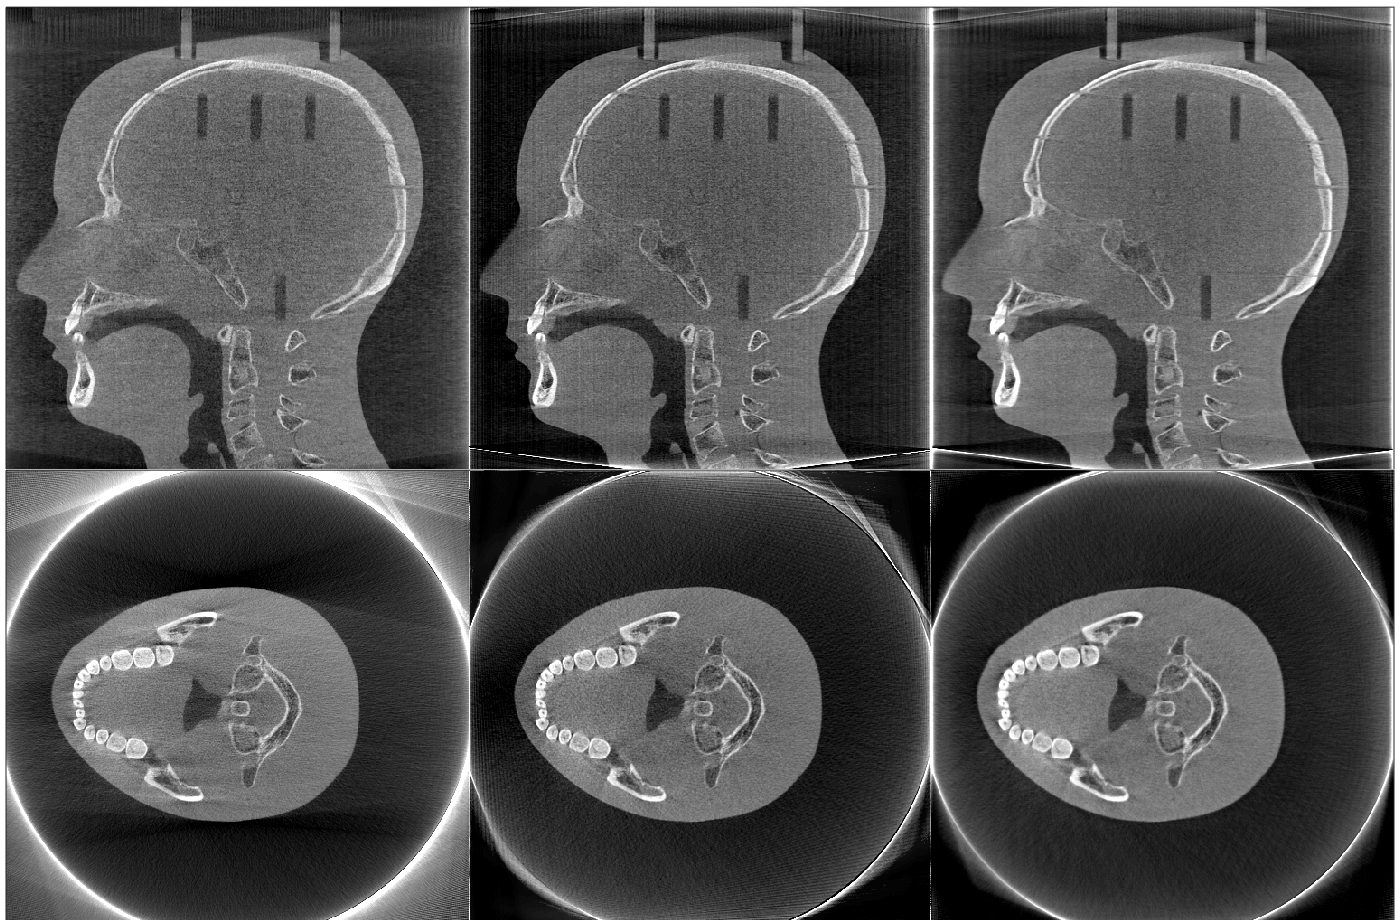
\includegraphics[width=0.98\textwidth]{GPUmethods/RANDO.png} };
\path (A.south west) -- (A.south east) node[pos=.175, below,align=center] {(a)\\ FDK \\14s total} node[pos=.5, below,align=center] {(b) \\OS-SART\\20m59s total\\31s per iteration} node[pos=.825, below,align=center] {(c)\\ CGLS \\ 6m8s total \\ 18s per iteration};
\end{tikzpicture}

\caption[RANDO head recosntructed in TIGRE using FDk,OS-SART and CGLS]{\label{fig:RANDOTIGRE} RANDO head phantom reconstructed with (a) FDK, (b) OS-SART 40 iterations and (c) CGLS 20 iterations, for 360 equidistant projections. The computational times are also shown.} 
\end{figure}



\subsubsection{Implementation of an algorithm in TIGRE}
To demonstrate the facility with which anyone can develop new algorithms using the
TIGRE toolbox, this section presents a side by side comparison of an algorithm definition and its TIGRE equivalent code, using the GPU accelerated features. For the
sake of brevity, the CGLS algorithm has been chosen.
In table \ref{tab:CGLSTIGRE} the definition of the CGLS iterations and the implementation in TIGRE
are shown. From the code snippet, it is worth highlighting the limited use of library related
functions, as one of the strengths of TIGRE for the developer point of view is the
easy to use Application Programming Interface (API). The only difference in the code
from a completely standard MATLAB script is the use of the function Ax() and Atb(),
the main building blocks of the toolbox. This allows anyone
with MATLAB code for solving image reconstruction to easily modify their code by just
changing the matrix-vector operations by TIGRE GPU functions. Note that the functions inside TIGRE do generally have more code than the one shown here, as several options and performance enhancing MATLAB tools are used.

\pagebreak


\begingroup
\captionof{table}{CGLS algorithm as definition, and implemented in TIGRE}\label{tab:CGLSTIGRE}
\endgroup
\begin{multicols}{2}
\begin{flalign*}
\label{eq:CGLSalgorithm}
%\begin{split}
&x_0=0; \; d_0=b; \; r_0=A^T b; p_0=r_0;&\\
&t_0=A r_0; \; \gamma_{k-1}=\left \| r_0 \right \|^2;&\\
&\textbf{for} \;k=1\; \textbf{to}\; k=\text{maxiter} &\\
&\;\;\;\; \alpha_k= \gamma_{k-1} / \left \| t_{k-1} \right \|^2 &\\
&\;\;\;\; x_k=x_{k-1}+\alpha_k t_{k-1}&\\
&\;\;\;\; d_k=d_{k-1}-\alpha_k t_{k-1}&\\
&\;\;\;\; r_k=A^Td_k &\\
&\;\;\;\; \gamma_k=\left \| r_{k} \right \|^2&\\
&\;\;\;\; \beta_k=  \gamma_{k} / \gamma_{k-1}&\\
&\;\;\;\; p_k=r_k+\beta_kp_{k-1} &\\
&\;\;\;\; t_k=Ap_k& \\
& \textbf{end}&
%\end{split}
\end{flalign*}
\columnbreak
\begin{lstlisting}[style=Matlab-editor,
basicstyle=\scriptsize,
label={cs:cgls},frame = single]
% Initialize variables
x=zeros(geo.nVoxel'); 
d=b;
r=Atb(b,geo,angles,'matched'); %TIGRE
p=r;
t=Ax(r,geo,angles); %TIGRE
gamma_1=norm(r(:));

% Loop until user defined maxiter
for k=1:maxiter
   alpha=gamma_1/norm(t(:));
   x=x+alpha*t;
   d=d-alpha*t;
   r=Atb(d,geo,angles,'matched');%TIGRE
   gamma=norm(r(:));
   beta=gamma/gamma_1;
   gamma_1=gamma;
   p=r+beta*p;
   t=Ax(p,geo,angles); %TIGRE  
end
% x is the solution.
\end{lstlisting}
\end{multicols}



\section{Summary}


In this chapter we have presented a MATLAB/CUDA toolbox for fast 3D X-ray image reconstruction. While the toolbox has reasonably good performance -- reducing to minutes an image reconstruction with complex iterative algorithms -- and a wide variety of tools, improvements are possible.

The projection and back projection operators have been fully implemented in the GPU, but the algorithms are fully in CPU so a memory management overhead exists because the data need to be introduced and extracted from the GPU twice per iteration. This design has been proposed in order to have the algorithms in a high-level language, as an algorithm implementation cycle in a low-level language like C++ is significantly longer than in MATLAB. As an estimate, if the algorithms were written in C++/CUDA directly, an improvement in computation time of up to 50\% could be achieved in some cases. However, this would increase the difficulty of adding new algorithms to the toolbox. The final decision was that the advantages of a high-level programming language for new algorithms are better than the possible benefits of doubling the speed, which is already reasonably good. 

Further improvements in the core GPU kernels of the toolbox would also be possible. While the speeds reached by this method are arguably state of the art, some improvements to the kernel structure to decrease even more memory latency and computational times have been proposed in the literature. It is impossible to know with certainty that any of the methods published will increase the speed of the code, partly because GPU architecture has changed over the past year massively, thus code may be faster in specific GPUs but slower in others, and partly because most of the published papers do not contain code to be benchmarked against, and use different geometric parameters each. Thompson and Lionheart\cite{thompson2014gpu} propose a method that exploits structure similarities and works if the cone angle is smaller than 45 degrees, that is the case of most commercial CBCT machines. The work in this thesis tries not to impose limitations on the possible geometries, but modifying the code to trigger the accelerated version proposed by Thompson and Lionheart is an interesting possibility. Chou \emph{et al}\cite{chou2011fast} claim speed-up by re-structuring the kernels to lauch multiple treads for multiple rays in parallel. While initial trials for replicating the multithreads in the early stages of the work in this thesis failed (as times where not changes) the projection operator has intensively been modified since then. This work has potential to accelerate up to 600\% the projection operation according to the article. Finally, the method proposed by Gao\cite{gao2012fast} claims significant speed-up over the ``naive'' Siddon's method, the code provided with their article shows slower execution for both the ``naive'' and accelerated versions than the code used in this work. Nevertheless, it would be worth implementing their approach.

The backprojection operator has been more optimized than the projection operation, using better techniques, thus speed-wise it is performing well. However, there are certainly faster methods, as TIGRE ranks between 5 and 7 in the RabbitCT\footnote{\href{https://www5.cs.fau.de/research/projects/rabbitct}{https://www5.cs.fau.de/research/projects/rabbitct} benchmark.} The RabbitCT benchmark is also recorded in different machines, thus some of the faster methods are due to multi-GPU parallelism exploits or just simply due to faster GPUs. That said, there is certainly room for improvement. 
Possibly the biggest improvement to the backprojection  would be the implementation of completely matched projection adjoint code, as it leads to better recosntruction\cite{6829349}. Thompson and Lionheart\cite{thompson2014gpu} propose a technique, so does Gao\cite{gao2012fast}.

Comparing the forward and back projection speeds to the ASTRA toolbox\cite{ASTRA}, TIGRE is 2 times slower at its worst. This can be easily explained by two factors. Firstly, the geometric options for CBCT are more flexible in TIGRE than in ASTRA, thus requiring more floating-point operations. Secondly, ASTRA implements an advanced ray splitting that increases memory latency in the GPU and that makes use of overlaps between X-ray paths at different angles\cite{Palenstijn2011250}. Adding all the discussed effects that would decrease the time performance, all algorithms run about 3 times more slowly in TIGRE than in ASTRA, which constitutes the state of the art. {Numerically, the differences between ASTRA and TIGRE are in absolute value of the order of $10^{-3}$, which is about 0.01\% in relative terms. This difference can be attributed to accumulated floating point errors due to different numerical approaches in the GPU code.}

To speed up further the toolbox, a multi-GPU approach could also be taken. Currently, TIGRE does not support multi-GPU architectures (there is a work in progress on it, lacking just final integration). A further weakness of the toolbox is the small number of functions for data loading and post-processing. However, work will be continued, hopefully filling this gap in the near future. The single GPU limitation of TIGRE also limits the image size. Currently, 12GB is the maximum amount of memory on a GPU board, thus limiting the possible size of the images that can be reconstructed. Nevertheless, there is no problem to reconstruct a $1024^3$ image with most algorithms so the maximum image size is still big.

The TIGRE Toolbox has been designed with the objective of reducing the gap between image reconstruction research and the end users of tomographic images. While research in reconstruction creates new algorithms every year, end users only have access to FDK implementations. With these two groups in mind, the toolbox:
\begin{itemize}
\item has easy-to-use ``black box'' algorithms, making it extremely straightforward for researchers who are only interested in the quality of the images to test different algorithms without them requiring any knowledge of how the algorithms work;
\item has easy-to-use building blocks (projection and back projection operators) that allow algorithm developers to test new methods using a high-level programming language but with the performance of the lowest level, GPU languages.
\end{itemize}
The code is released as open source under a BSD 3-clause license, allowing anyone to download, test, modify and improve it. While the toolbox was originally designed for CBCT image reconstruction, an option for 3D parallel-beam CT reconstruction has also been included allowing for more geometries, e.g., synchrotron data. Further tweaking the geometry structure of the toolbox also permits 2D fan- and parallel-beam reconstructions.

% We enthusiastically encourage the submission of improvements, bug-fixes, demos, data and whatever else might help the community. Likewise, we encourage algorithm developers to submit their new algorithms to the toolbox, giving them visibility. Finally, we would like to encourage X-ray image end users to include data or descriptions of specific challenges they may have, allowing dialogue and hopefully leading to better ways of creating enhanced tomographic images. 

The minimum requirements to run the toolbox are strongly dependent on the image size desired, as memory is the strongest limiting factor both on the CPU and GPU side. Generally speaking, any NVIDIA GPU with a compute capability higher than 3.5 would be sufficient to reconstruct arbitrarily large images. We recommend having at least 3 times the desired image size in GPU memory and 8 times in RAM in the computer. As an example, for a $512^3$ image, 2GB of GPU memory and 6GB of computer RAM is the suggested minimum. The computing power (number of processors in the GPU and processor performance of the CPU) will have a strong effect on the speed of image reconstruction. 


%Projection:


%While there is potential for improvement, the speeds achieved with the code in developed are fast enough (see section \ref{sec:speed} for speed tests) for the intended purposes in this work.\label{ch:GPU}
\chapter{Experiments and Applications}

In the previous two chapters the mathematical and computational challenges of image reconstruction for CT have been discussed. In chapter 3, a detailed description of a variety of different algorithms has been presented, including the ART family of algorithms, CGLS, MLEM and few TV approaches for smooth reconstruction, as well as the classic FDK reconstruction. Additionally in chapter 4 the computational aspect of CT is discussed, on where the problems computing the exact adjoint of the projection operation and mainly the computational burden of some of the operations have been mentioned. Considering the variety of available methods and the specifics of the implementation of the software developed, the TIGRE toolbox, experiments on how these algorithms compare and behave are due. Further than that, the performance of these algorithm in different experimental datasets is also an important analysis.

This chapter shows experimental analysis on both of the topics. First a variety of convergence analysis with different algorithms using synthetic data are performed, showing the differences not only between algorithms, but also between option on parameter selections. The section tries to illustrate and perhaps help build intuition on all the different parameters and options that each of these algorithms has, both within the algorithms themselves and among the different ones. Additionally some highlights on the practical challenges that the use of the algorithms entail in real applications are given.

In the second section of this chapter, a few examples of some of the algorithms are shown in different CT applications, both cone and parallel beam. Data from various different applications, from medicine to science has been tested using the TIGRE toolbox. While quantitative analysis is not possible with these datasets because the truth is not known, some insight in how the algorithms behave in each case is discussed.

\section{Algorithm Experiments}
This section experiments with a variety of algorithms and parameter within then, and shows how they behave with different synthetic data in simulation studies. 

\subsection{Convergence rates}

On chapter 3 the convergence rates of the algorithms has been mentioned, as well as computational times. Different algorithms will reach to different residuals at the same iteration, and thus understanding which ones can converge faster, thus theoretically give a better result earlier, is important. However, at the scale of the CBCT problem, faster no only means reaching a residual that is smaller in the same iterations, as the computational burden of each of the iterations also needs to be considered. And, as the backprojection operator is not exactly the adjoint of the projection operator, an effect that the classic formulation of these algorithms do not take into account can happen: divergence. All the algorithms (at least in this work) are mathematically designed to always reduce the residual each iteration, but that formulation relies on a correct adjoint operator. Thus, sometimes, when the algorithms in TIGRE have a solution very close to minimum residual solution, they may diverge. The code in the toolbox does generally check for divergence and stop, but one of the effect that can be observed is that some algorithm will always diverge in a residual that is larger than others. This means that some algorithm can, regardless of their computational times, reach to a better solution than others.

All test in this section are performed in the XCAT phantom\cite{XCAT}, in a $128^3$ voxel size and $256^2$ detector. Different number of angles are used, always uniformly distributed along the full circle. Figure \ref{fig:XCAT} shows cross sections of the phantom on its middle plane and figure \ref{fig:XCATproj} shows 3 projections of the phantom as simulated for the following tests. 

\begin{figure}[h]
\begin{center}

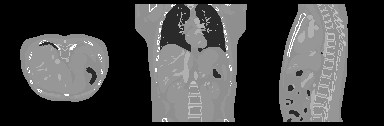
\includegraphics[width=0.9\textwidth]{Applications/XCAT.png} 
\end{center}

\caption[Cross section of the XCAT phantom]{\label{fig:XCAT} Cross section of the XCAT phantom in its middle plane in the three axis, for $128^3$ voxels.} 
\end{figure}

\begin{figure}[h]
\begin{center}

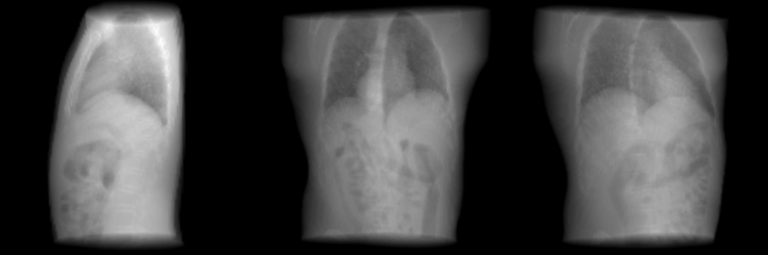
\includegraphics[width=0.9\textwidth]{Applications/XCATproj.png} 
\end{center}

\caption[Simulate projections of the XCAT phantom]{\label{fig:XCATproj} Simulate projections of the XCAT phantom in three different projection angles for a $256^2$ detector.} 
\end{figure}

\textbf{Update ordering in SART}. An analysis in the different ART-type algorithms is presented in this section first. One of the discussed parameters that has an effect in the convergence rate of the ART-type algorithms is the ordering of the used projections. Research has shown that in ART, the decrease of the residual with respect to how the rows are chosen for the updates is significantly changed[CITE], however in the algorithms feasible for big scale tomography, this effect is seen in a smaller scale. Figure \ref{fig:SARTanglesconv} shows the convergence of SART during 150 iterations using 100 projections as data. The same configuration of SART is run using ordered, randomly ordered and angular distance maximizing ordering schemes for the update order. While minor, the figure shows how random ordering does generally increases the convergence rate of the algorithm, at no computational cost. This is the default value in the software. Note that in this test there is no reduction of the relaxation parameter $\lambda$.


\begin{figure}[H]
\begin{center}

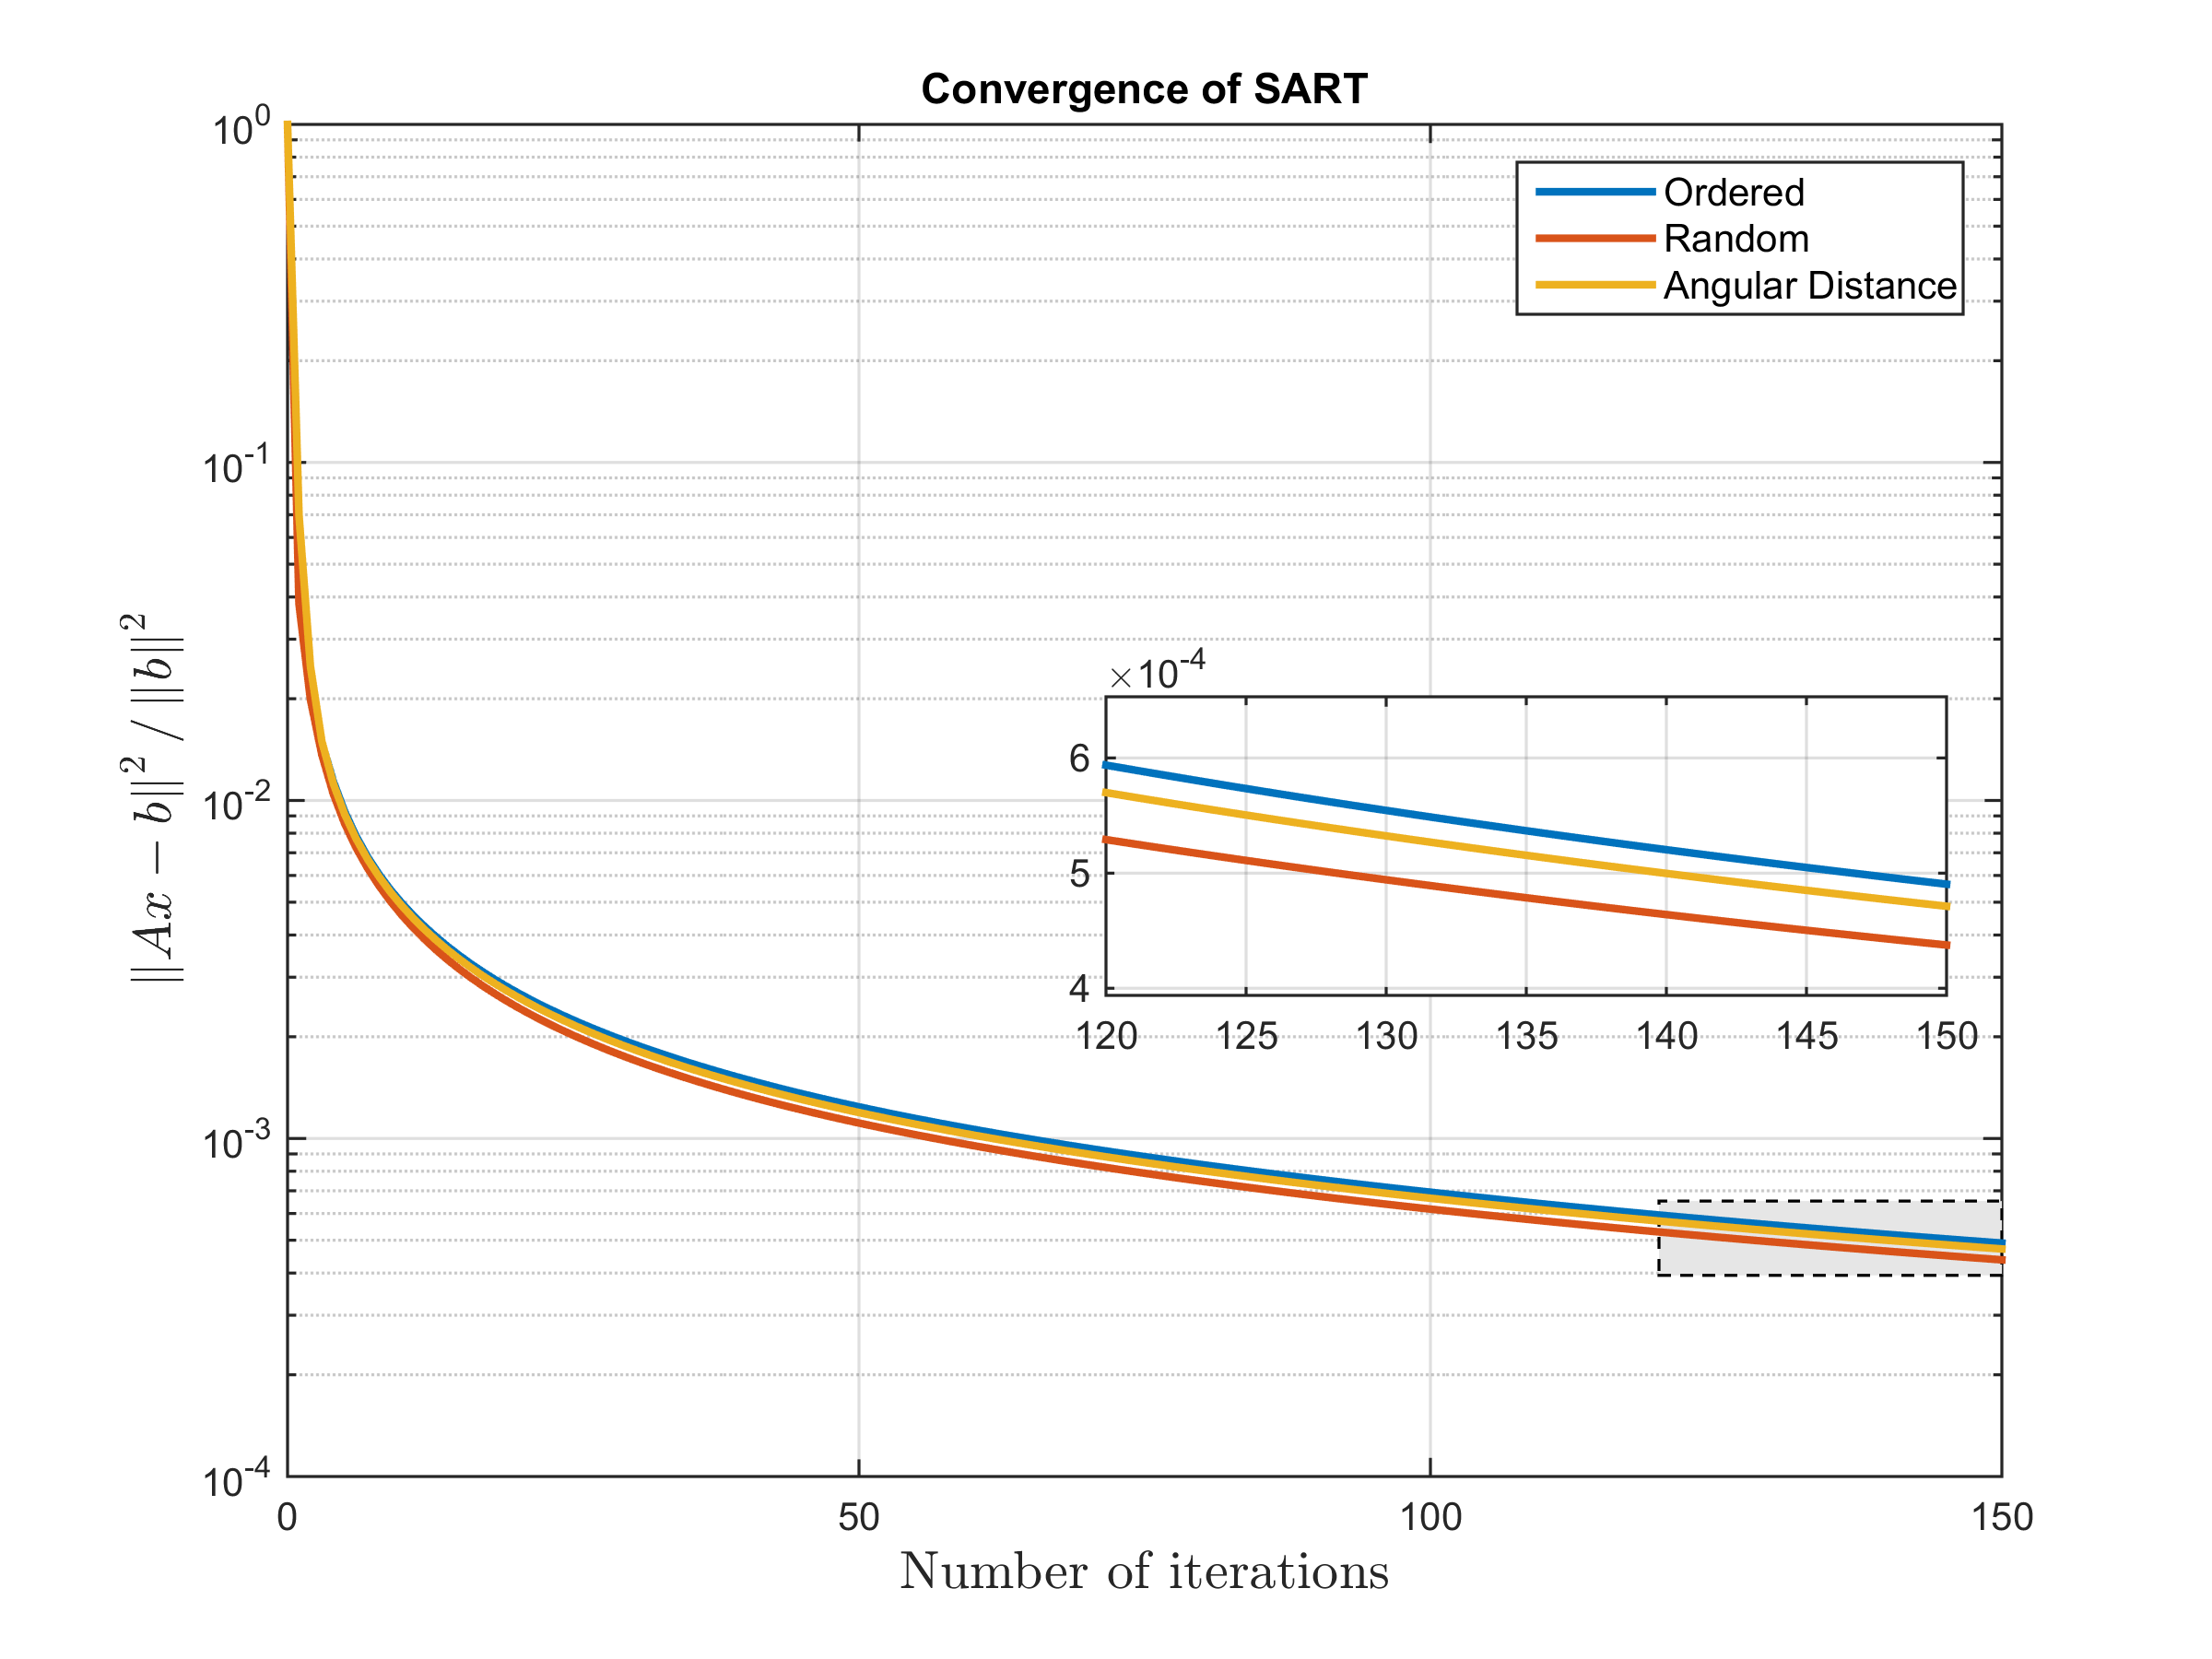
\includegraphics[width=0.8\textwidth]{Applications/SARTangles.png} 
\end{center}

\caption[Nomralized residual vs iteration of SART vs projection update order]{\label{fig:SARTanglesconv} Normalized residual versus iteration of SART compared to different angle ordering schemes, using 100 projections and no relaxation parameter reduction} 
\end{figure}

\textbf{Comparison between SART, OS-SART and SIRT}. These algorithms have very different convergence, as updating the image per-equation has the effect of converging faster. However, the computational times are greatly reduced by updating more rows at the same time. This effect can be seen in figure \ref{fig:SARTtypesconv}, on where the convergence versus iteration of these three algorithms is plotted. Note the convergence difference between SART and SIRT, where SIRT doesn't reach SART's residual even after 1000 iterations, however, each iteration of SIRT is two orders of magnitude faster than SART. OS-SART provides a middle ground alternative. Due to the specifics of the acceleration procedures for backprojection, OS-SART speeds are closer to SIRT than to SART (i.e. the speed does not change linearly with the image updates per iteration), however it is more prone to divergent behaviour in TIGRE. In the figure, OS-SART stops converging after 48 iterations. Of course, this behaviour is very data-specific, and there are multiple cases where it does not diverge. Figure XX shows the result images of these three algorithms after 150 iterations (48 for OS-SART). Note that the example being show is low data, so even in the best case, the images are slightly noisy.



\begin{figure}[H]
\begin{center}

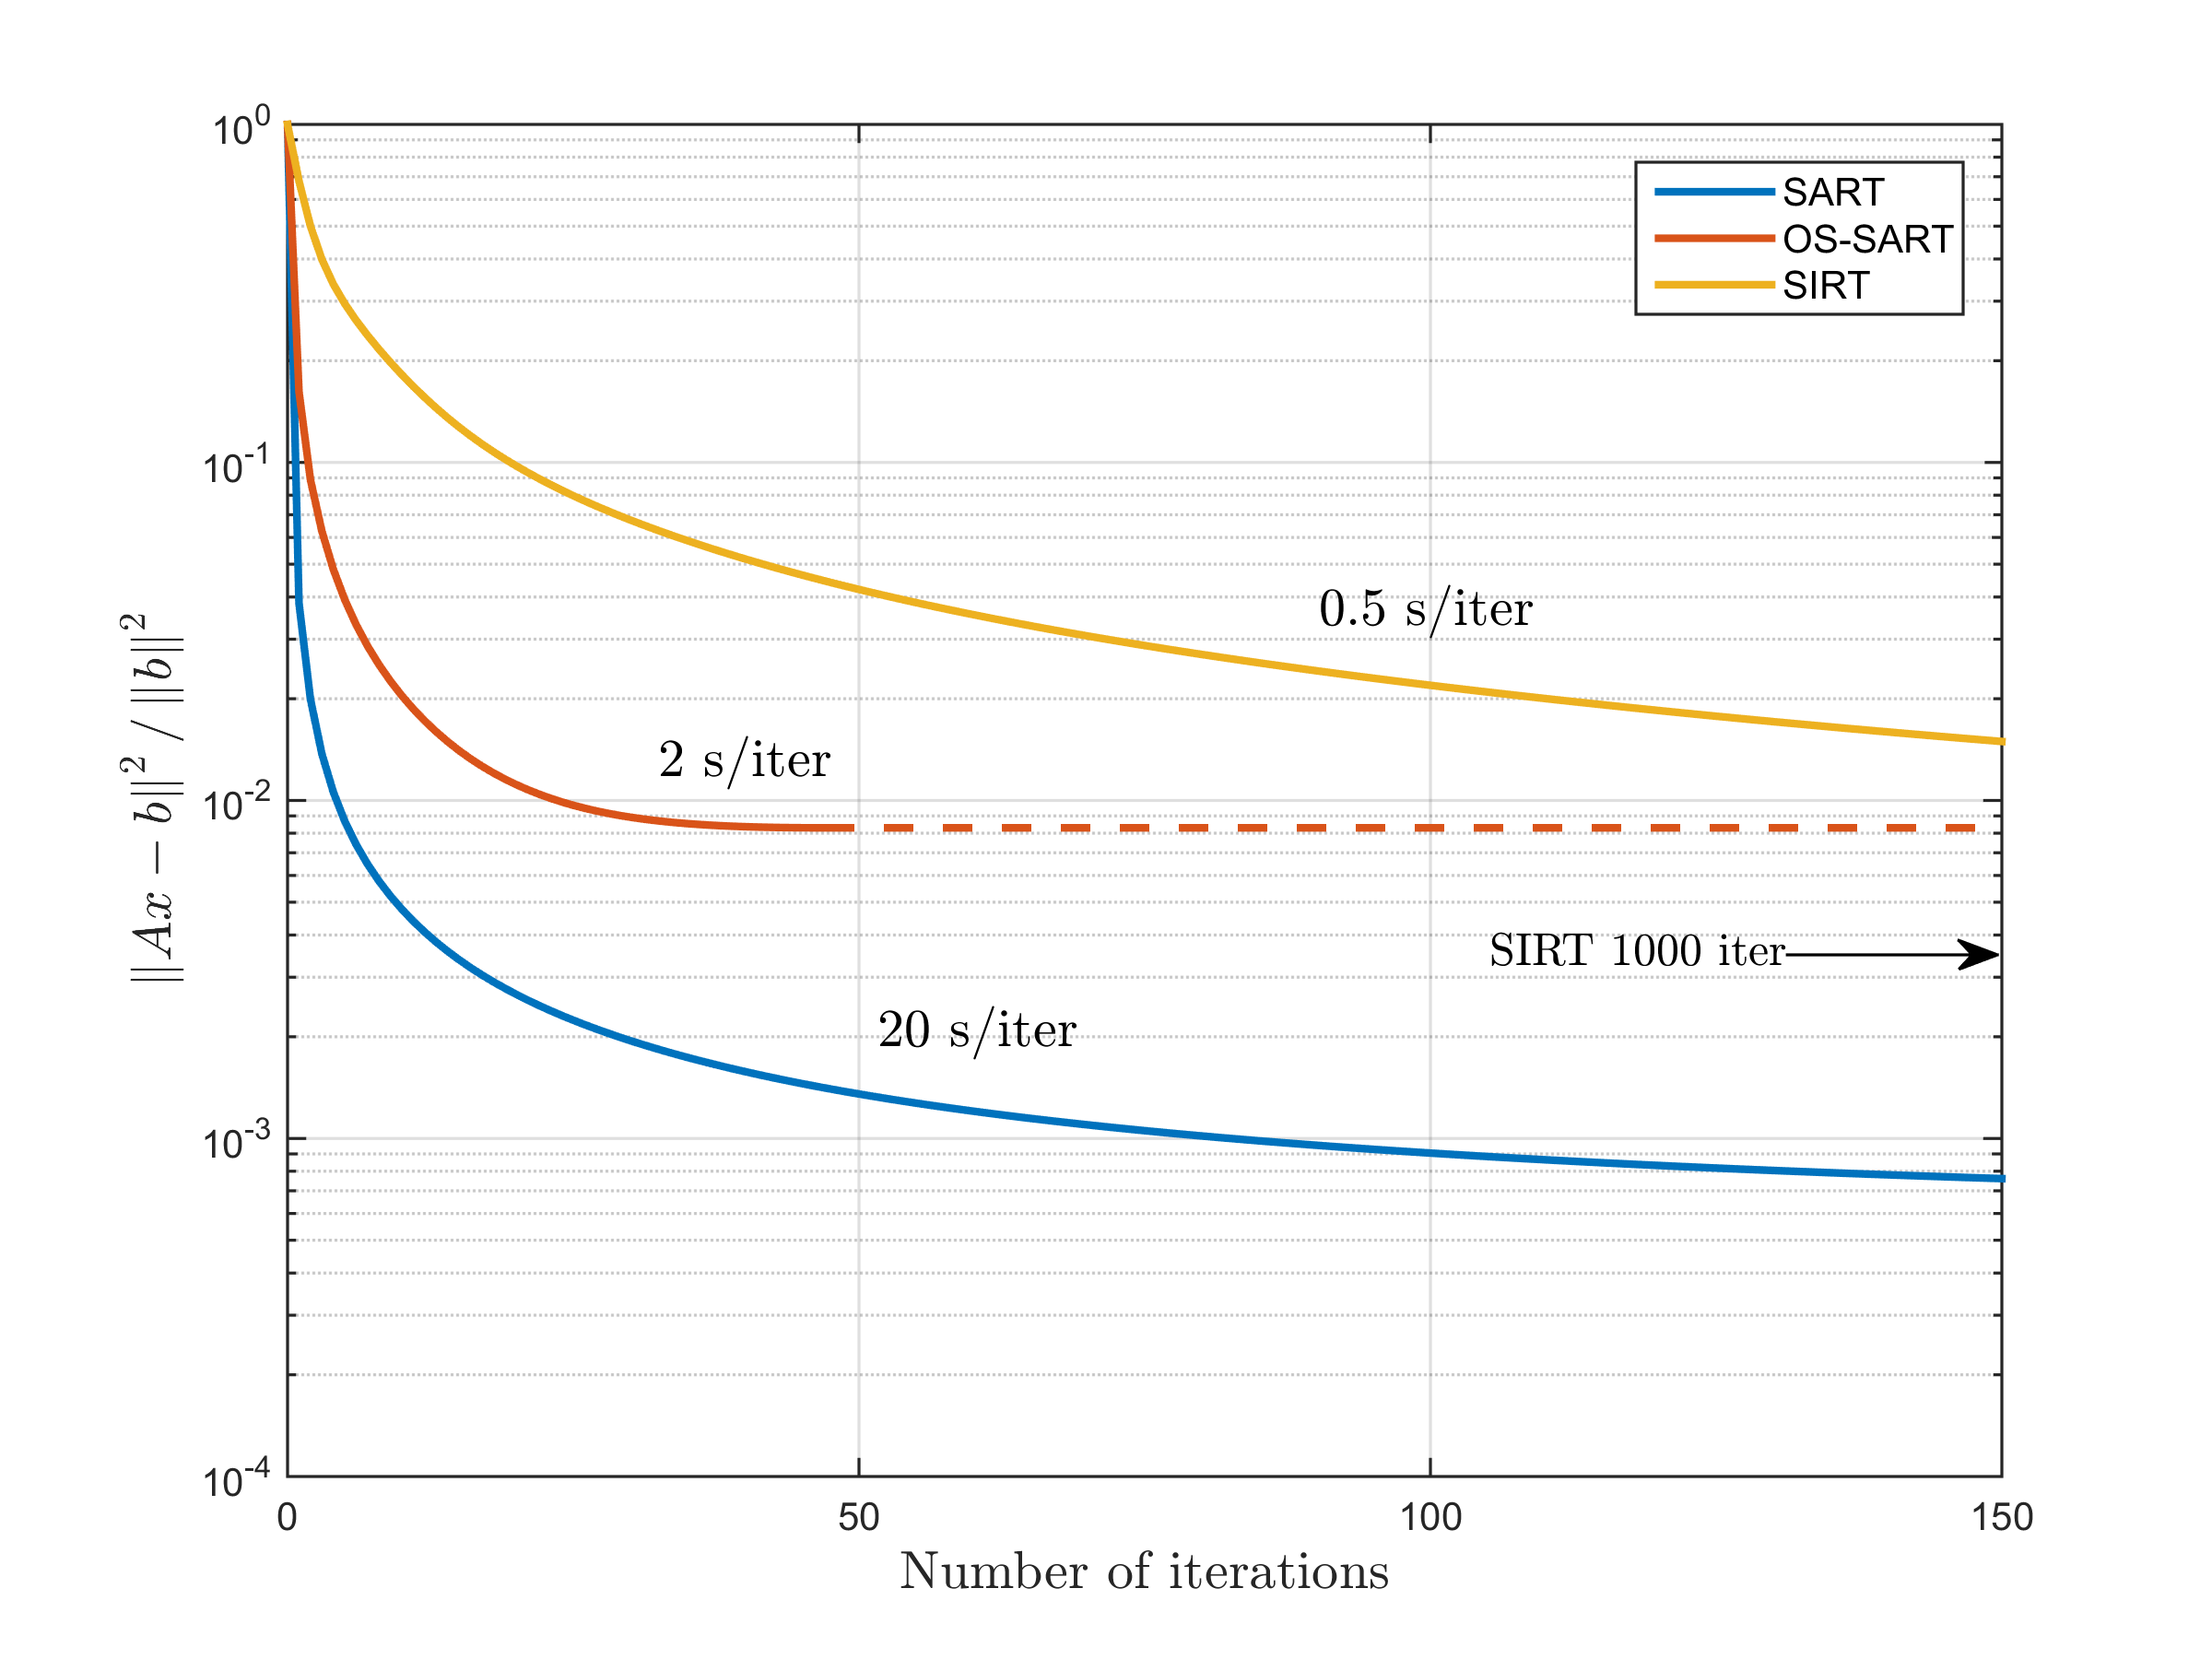
\includegraphics[width=0.8\textwidth]{Applications/SARTtypes.png} 
\end{center}

\caption[Nomralized residual vs iteration of SART/OS-SART/SIRT]{\label{fig:SARTtypesconv} Normalized residual vs iteration number for SART, OS-SART and SIRT using 100 projections and no relaxation parameter reduction.} 
\end{figure}

\textbf{Relaxation parameter.} The choice of a proper relaxation parameter does significantly change the speed on which a solution is found, and can avoid infinitely iterating through the same hyperplanes in case of an under determined or noisy solution. In TIGRE, two methods are present, as described in chapter 2: multiplying the relaxation parameter by a reduction factor after each iteration, and the Nesterov accelerated update, that does not technically update the relaxation parameter, but updates the image in each iteration using a iteration specific combination ration of the gradients of the current and previous iteration. It requires more memory, as it needs one extra image-sized variable to store the previous update, but the the algorithm finds a solution considerably faster, as it can be seen in figure \ref{fig:SARTlambda}. In the figure each of the SART, OS-SART and SIRT algorithms residual is plotted, and in each of them three versions are displayed, no relaxation parameter update, reduction with $r_{red}=0.99$ and Nesterov update. In the plot it can also be seen that reducing the relaxation parameter by a ratio, while a good approach in SART-based hybrid algorithms, such as the TV minimizing ones in TIGRE, leads with slower residual reduction and ultimately with a worse image.

In figure \ref{fig:SARTlambdaplot}, the solution found by the three algorithms using reduction of the relaxation parameter, using a Nesterov update and using static relaxation parameter of $\lambda=1$ can be seen side to side . The superior solution found by Nesterov is visually clear, and both SART and OS-SART reach a minimum in very few iterations. While SART does reach a better image (both in residual and error) without using Nesterov's update, the difference is minimal. It is important to note that using Nesterov's update, likely due to its fast convergence, leads to a faster divergent behaviour by the algorithms, thus the residual needs to be checked in each iteration leading to some computational overheat.

\begin{figure}[H]
\begin{center}

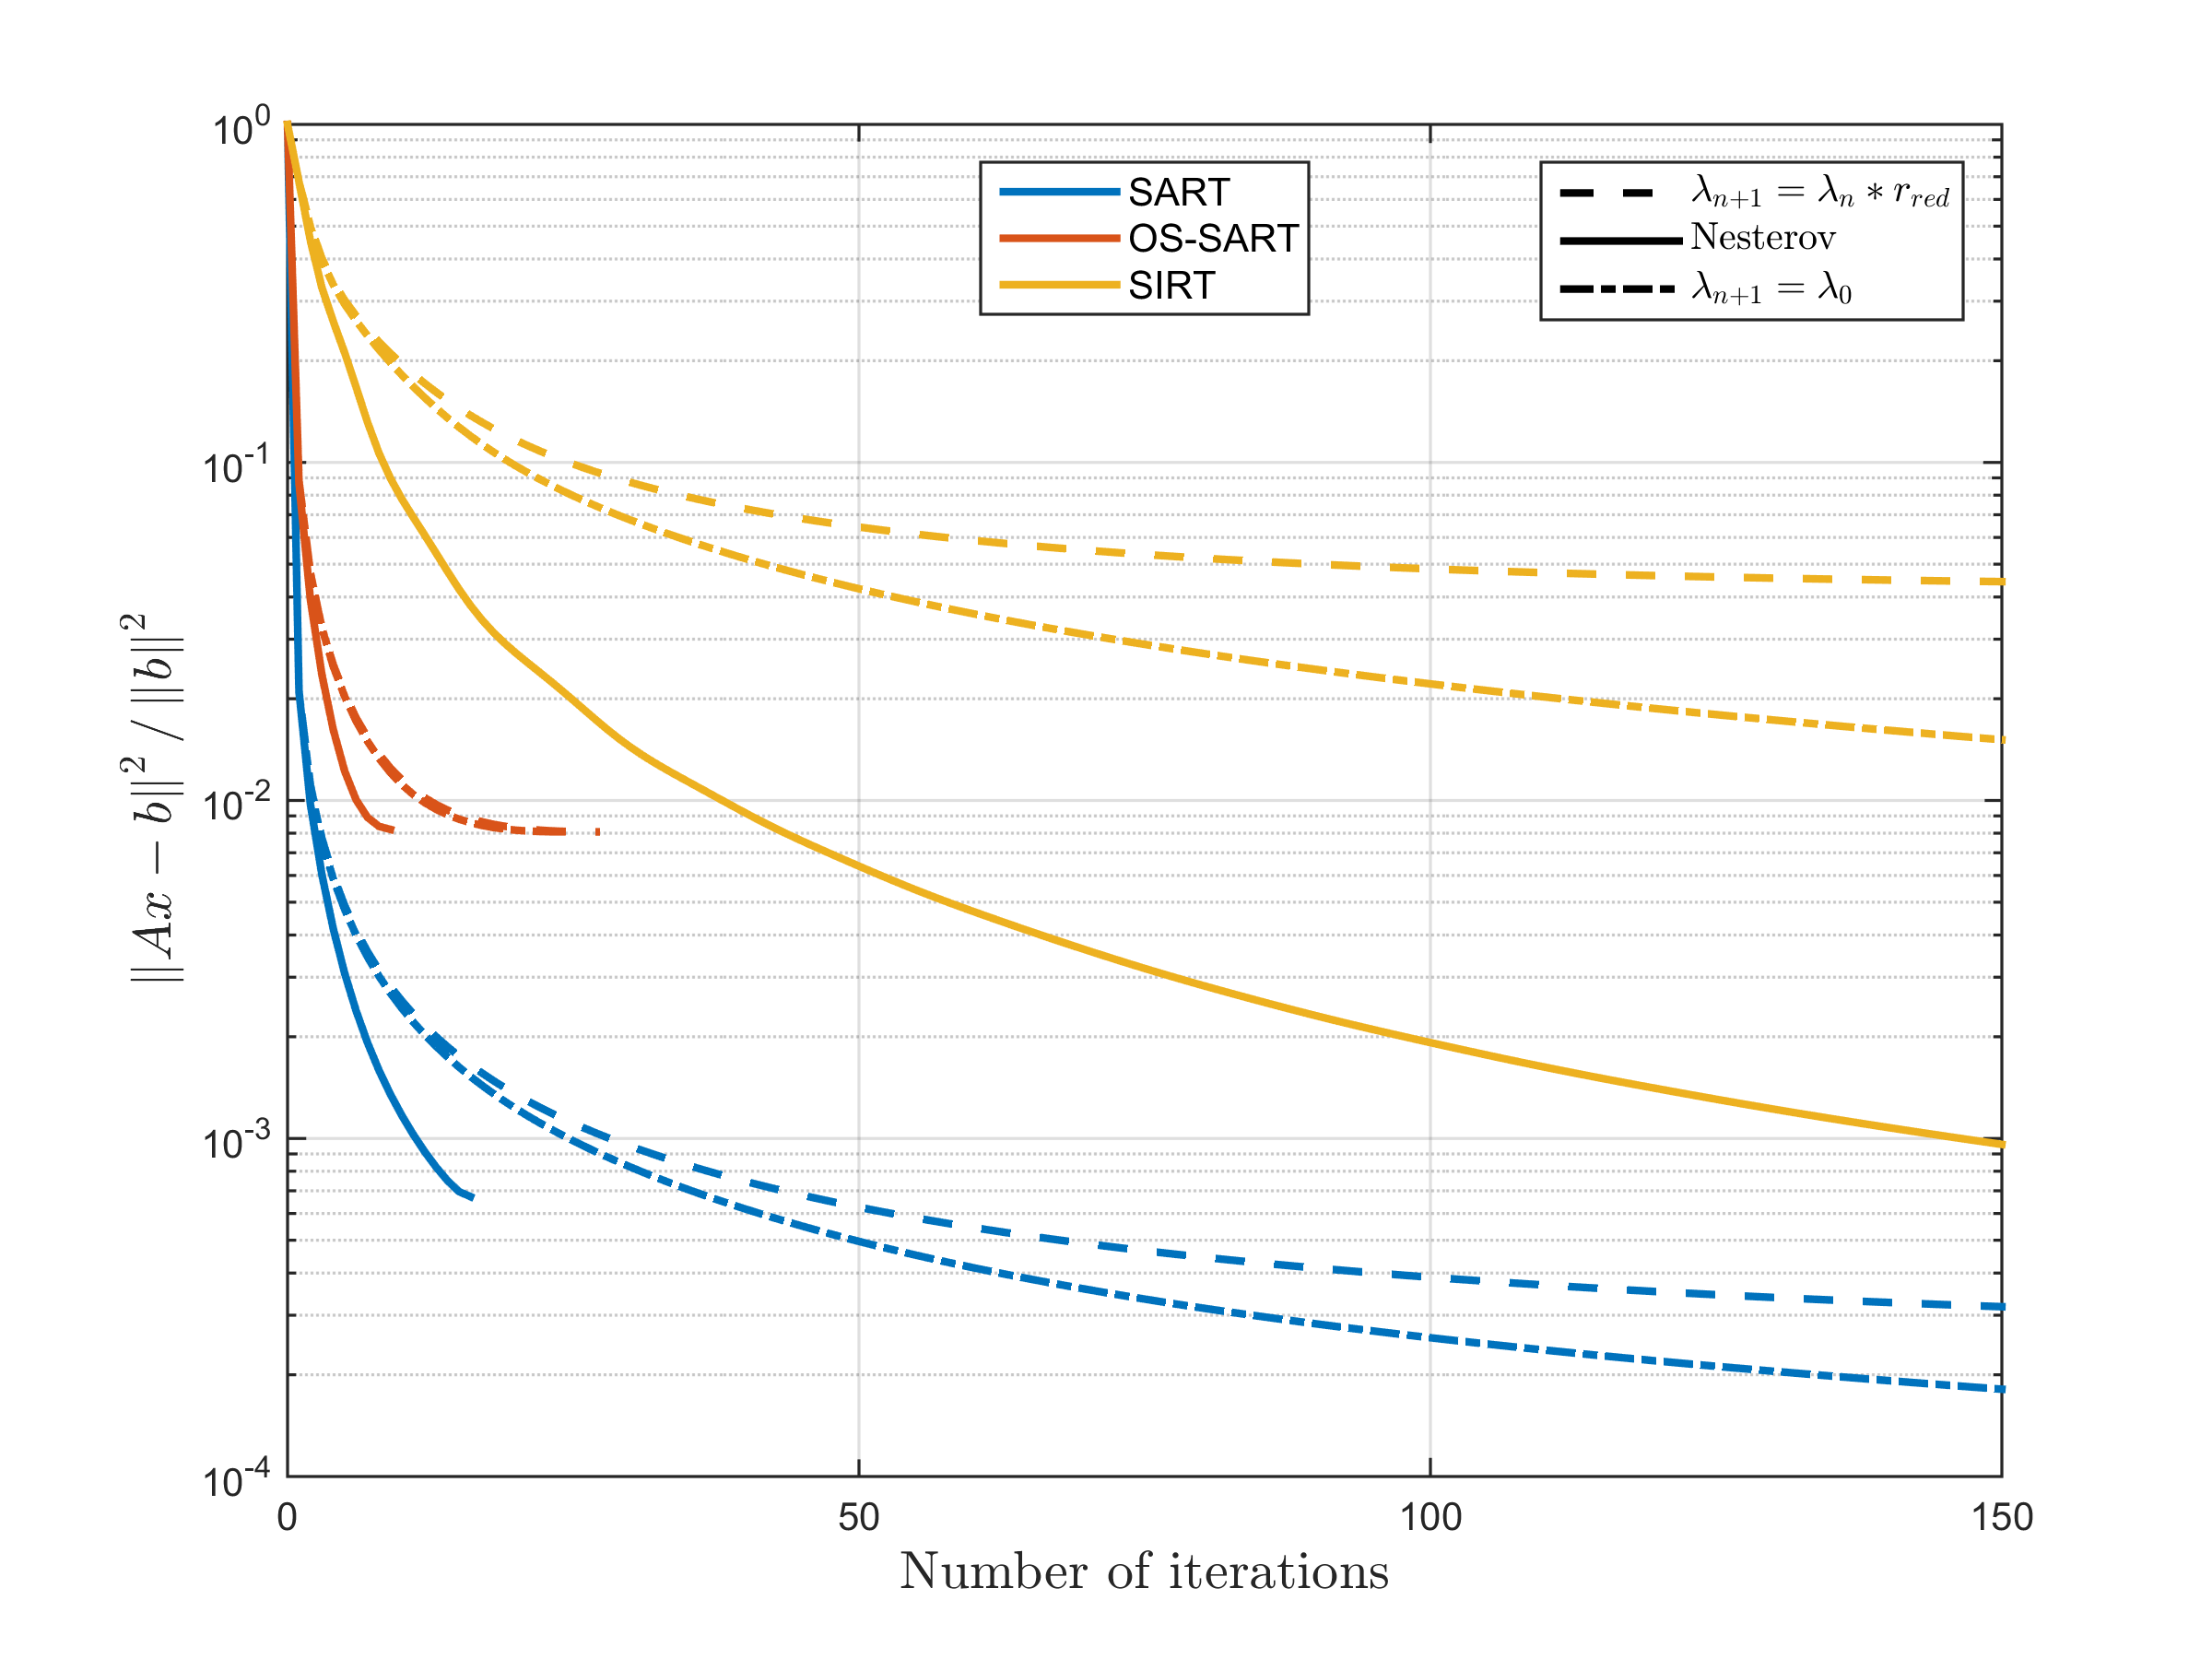
\includegraphics[width=0.8\textwidth]{Applications/SARTlambda.png} 
\end{center}

\caption[Nomralized residual vs iteration of SART/OS-SART/SIRT with different relacation parameters]{\label{fig:SARTlambda} Normalized residual vs iteration number for SART, OS-SART and SIRT using 100 projections and different relaxation parameter reduction modes. If the relaxation parameter is reduced by a constant ratio the residual reduction worsens, and if reduced using Nesterovs update, it converges very fast.} 
\end{figure}


\begin{figure}
\centering
\begin{tikzpicture}

\node (A) {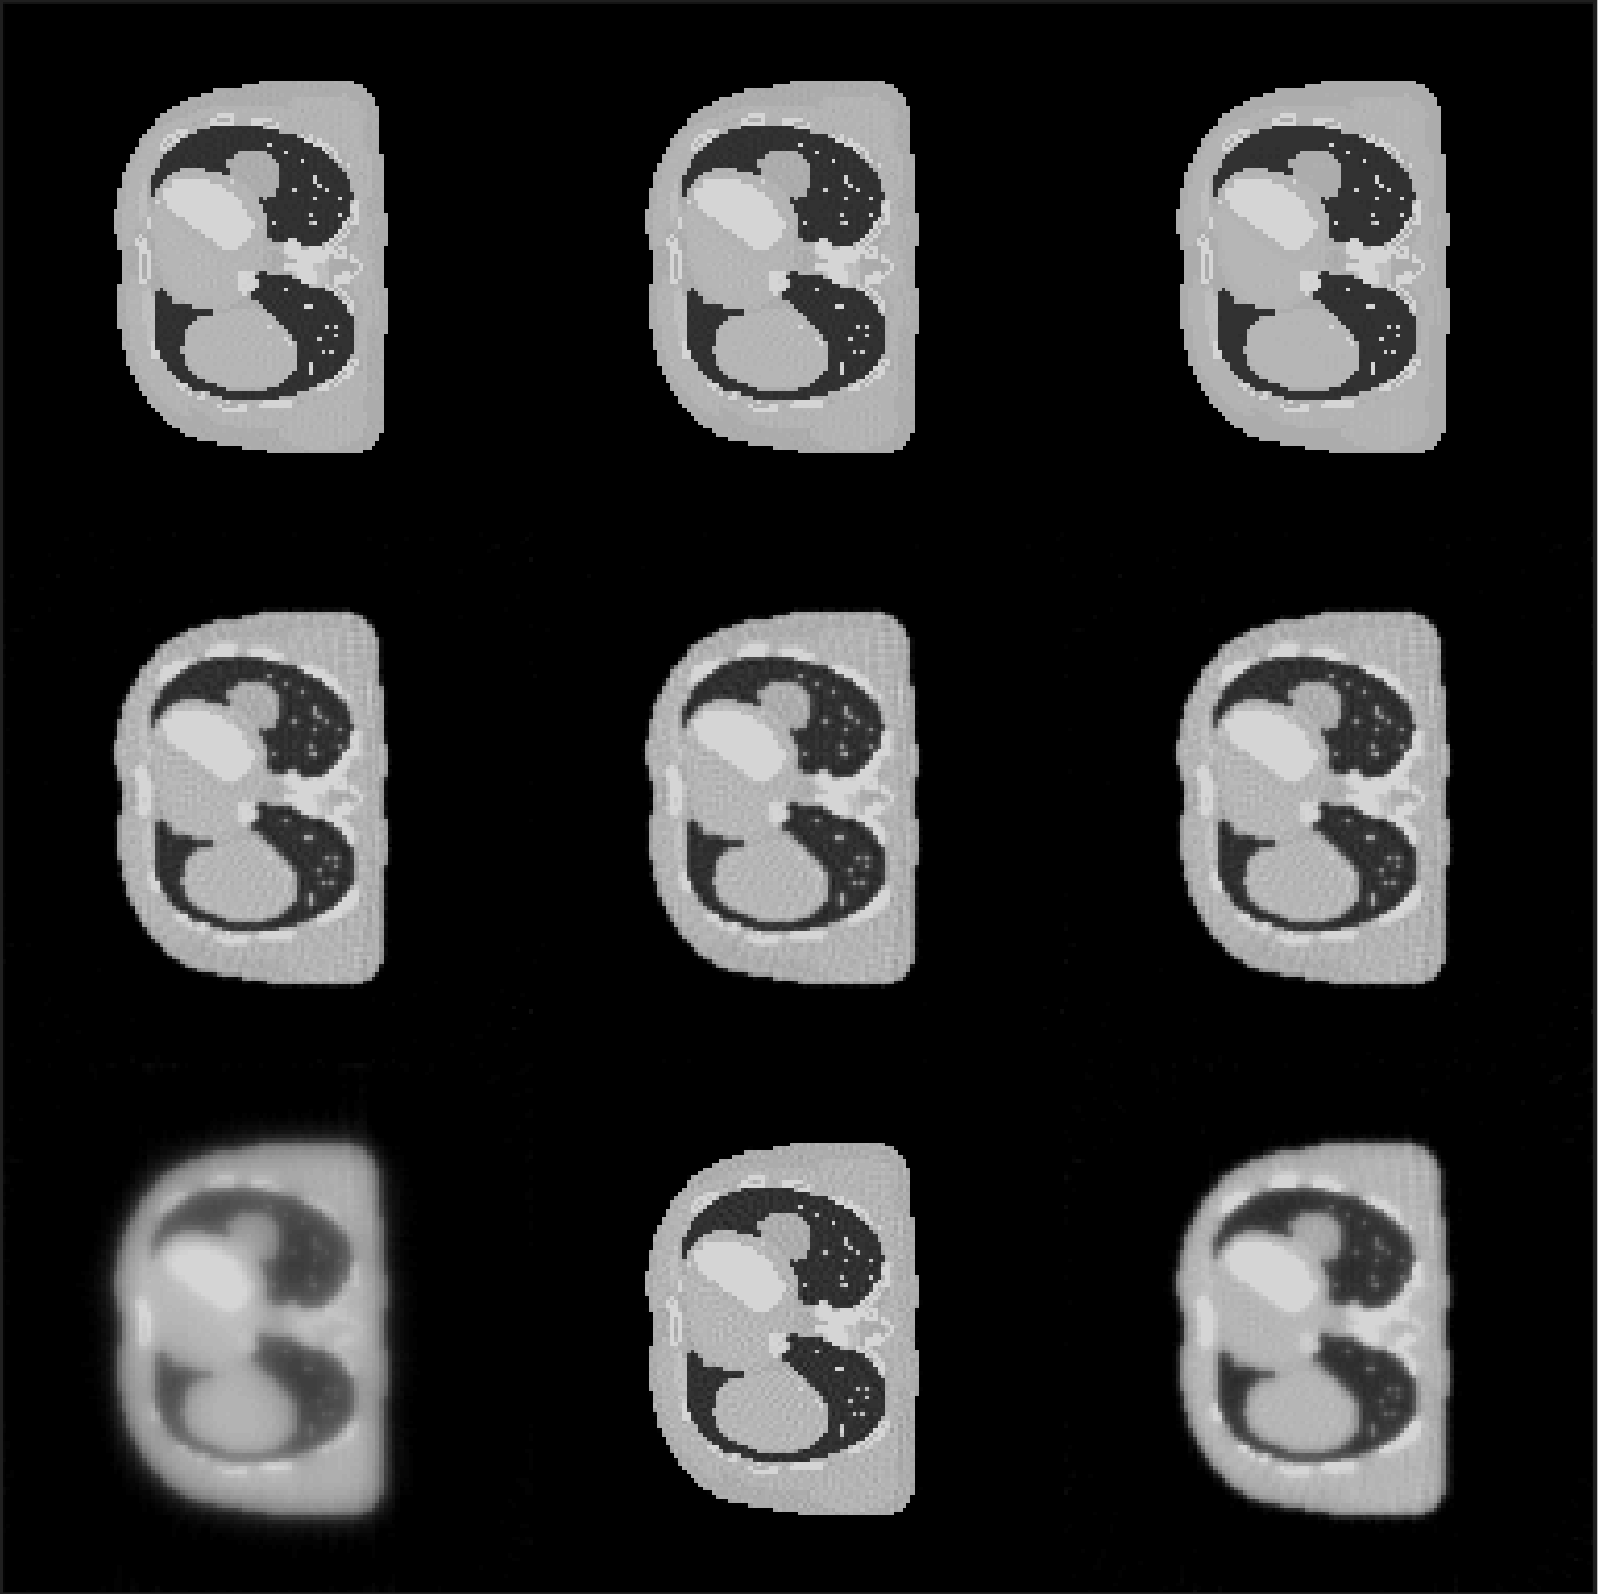
\includegraphics[width=0.94\textwidth]{Applications/SARTlambdaplot2.png} };
\path (A.south west) -- (A.north west) node[pos=.18, above, rotate=90] {SIRT} node[pos=.5, above, rotate=90] {OS-SART} node[pos=.82, above, rotate=90] {SART};
\path (A.south west) -- (A.south east) node[pos=.18, below] {$\lambda_{n+1}=\lambda_{n}*r_{red}$} node[pos=.5, below] {Nesterov} node[pos=.82, below] {$\lambda_{n+1}=\lambda_0=1$};

\end{tikzpicture}
\caption[Reconstructed images with different relaxation parameter updates]{\label{fig:SARTlambdaplot}Reconstructed images with different relaxation parameter updates. OS-SART stops at iteration 24 in all but in the Nesterov case, where it stops in the iteration number 9. SART stops at iteration number 16 for Nesterov.}
\end{figure}



\subsection{Total variation minimization}
There are 4 total variation minimizing algorithms in TIGRE, with 2 different minimization functional in total. As previously described, ASD-POCS, OS-ASD-POCS and b-ASD-POCS-$\beta$ minimize the TV using a POCS minimization technique by minimizing the data constrain and TV norm independently using gradient descend. SART-TV however uses the ROF model for the TV-minimization step. The total variation algorithms are designed for applications on where the image is piecewise-smooth, as they will try to minimize the gradient on the image, by creating single valued patches in the image. In CT, the most noisy images are reconstructed when either the data is very noisy (generally due to small acquisition times and/or low energy X-rays) or when the data is limited, either from limited angle or more importantly limited amount of projections. 

An example of the behaviour of the TV algorithms with the same dataset as in figures \ref{fig:XCAT} and \ref{fig:XCATproj} is shown in figure \ref{fig:TVXCAT}. In this case, 30 uniformly sampled projections are used, perturbed with Poisson and Gaussian noise, to simulate photon scattering and electronic noise respectively. The figure shows FDK and OS-SART reconstructions, and the 4 mentioned TV algorithms. It is visually clear that the TV algorithms do provide a smoother reconstruction, and with less Normalized root mean squared error (NRMSE), as seen in table \ref{tab:NRMSE TVs}.
The reconstruction by FDk is plagued with noise, and while the main structural features can be seen, most of the detail is lost. Even the bones themselves are practically indistinguishable from noise. OS-SART does reconstruct a smoother image, something predictable as it minimizes de 2-norm, and while one can see the more details in the image, it is still low. The rest 4 TV algorithms can be seen to flatten out the attenuation levels to similar values, thus reducing most of the noise. Additionally most of the features get clearly separated from the attenuation levels of the surrounding tissues and some of the algorithms (such as ASD-POCS) are able to reconstruct even single wide pixel structures correctly. It is important to note that while the parameters used to tune this specific TV reconstruction (available in the demo number 9 in the TIGRE toolbox), they are far from optimal and very sensitive\cite{Vee}. When choosing the exact optimal parameters for the TV reconstruction algorithms, the result images tend to be significantly better than the ones shown here, but the parameter space is very data dependant and massive, thus to the author's knowledge, no parameter selection method has been proposed in the literature. 


\begin{figure}
\centering
\begin{tikzpicture}

\node (A) {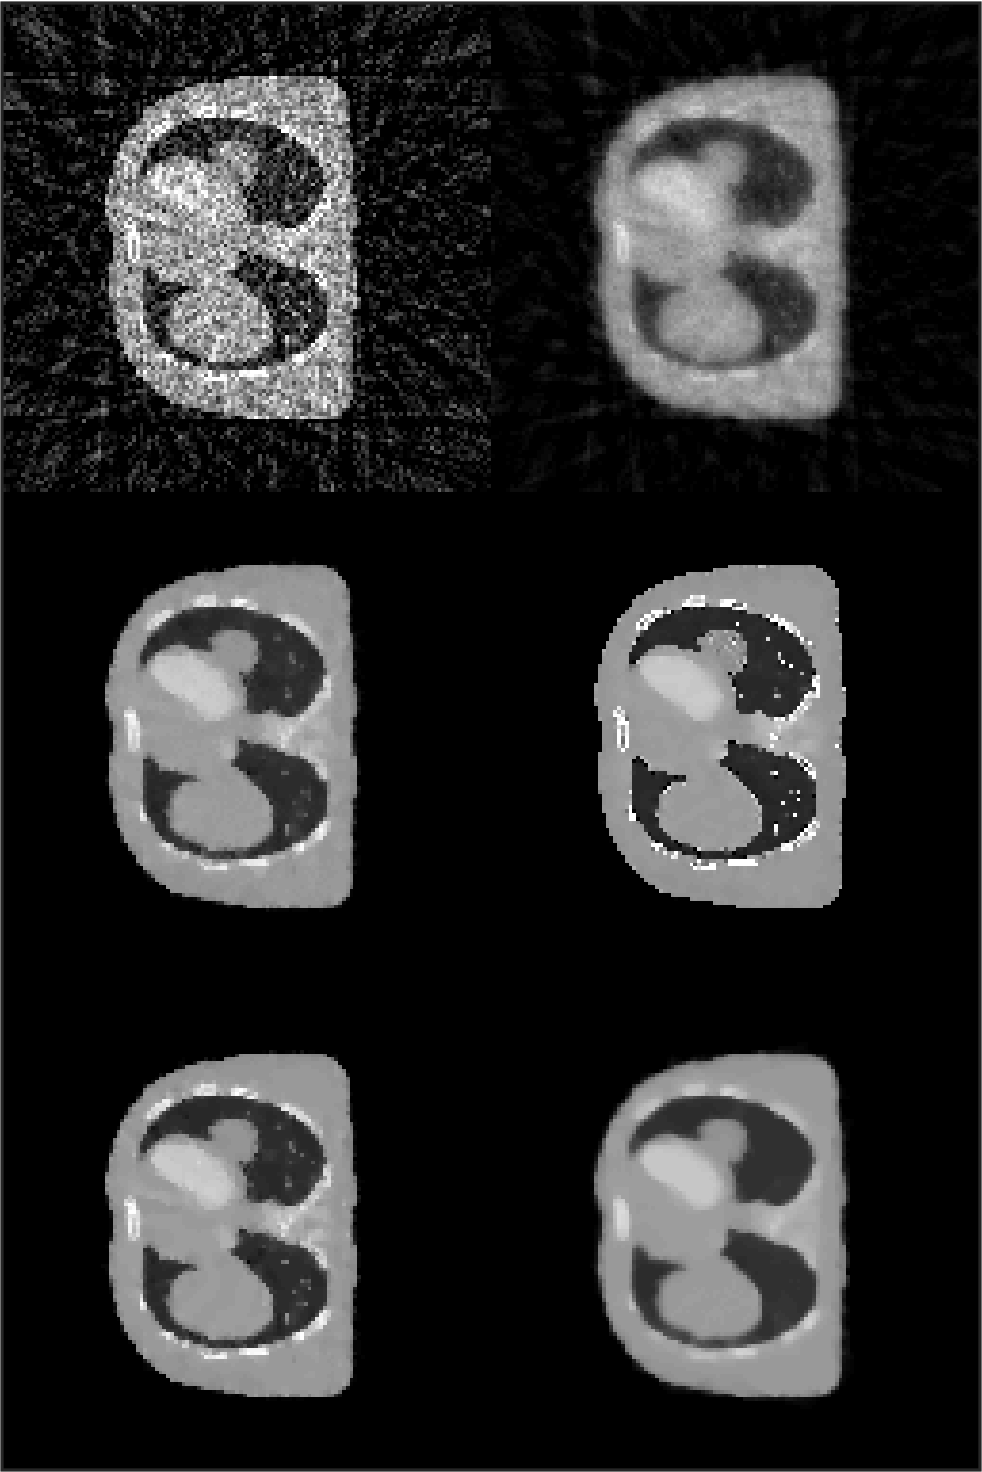
\includegraphics[width=0.4\textwidth]{Applications/TVs.png} };
\path (A.south west) -- (A.north west) node[pos=.18, above, rotate=90] {ASD-POCS} node[pos=.5, above, rotate=90] {b-ASD-POCS-$\beta$} node[pos=.82, above, rotate=90] {FDK};
\path (A.south east) -- (A.north east) node[pos=.18, below, rotate=90] {OS-ASD-POCS} node[pos=.5, below, rotate=90] {SART-TV} node[pos=.82, below, rotate=90] {OS-SART};

\node (B)at (0.5\textwidth,0) {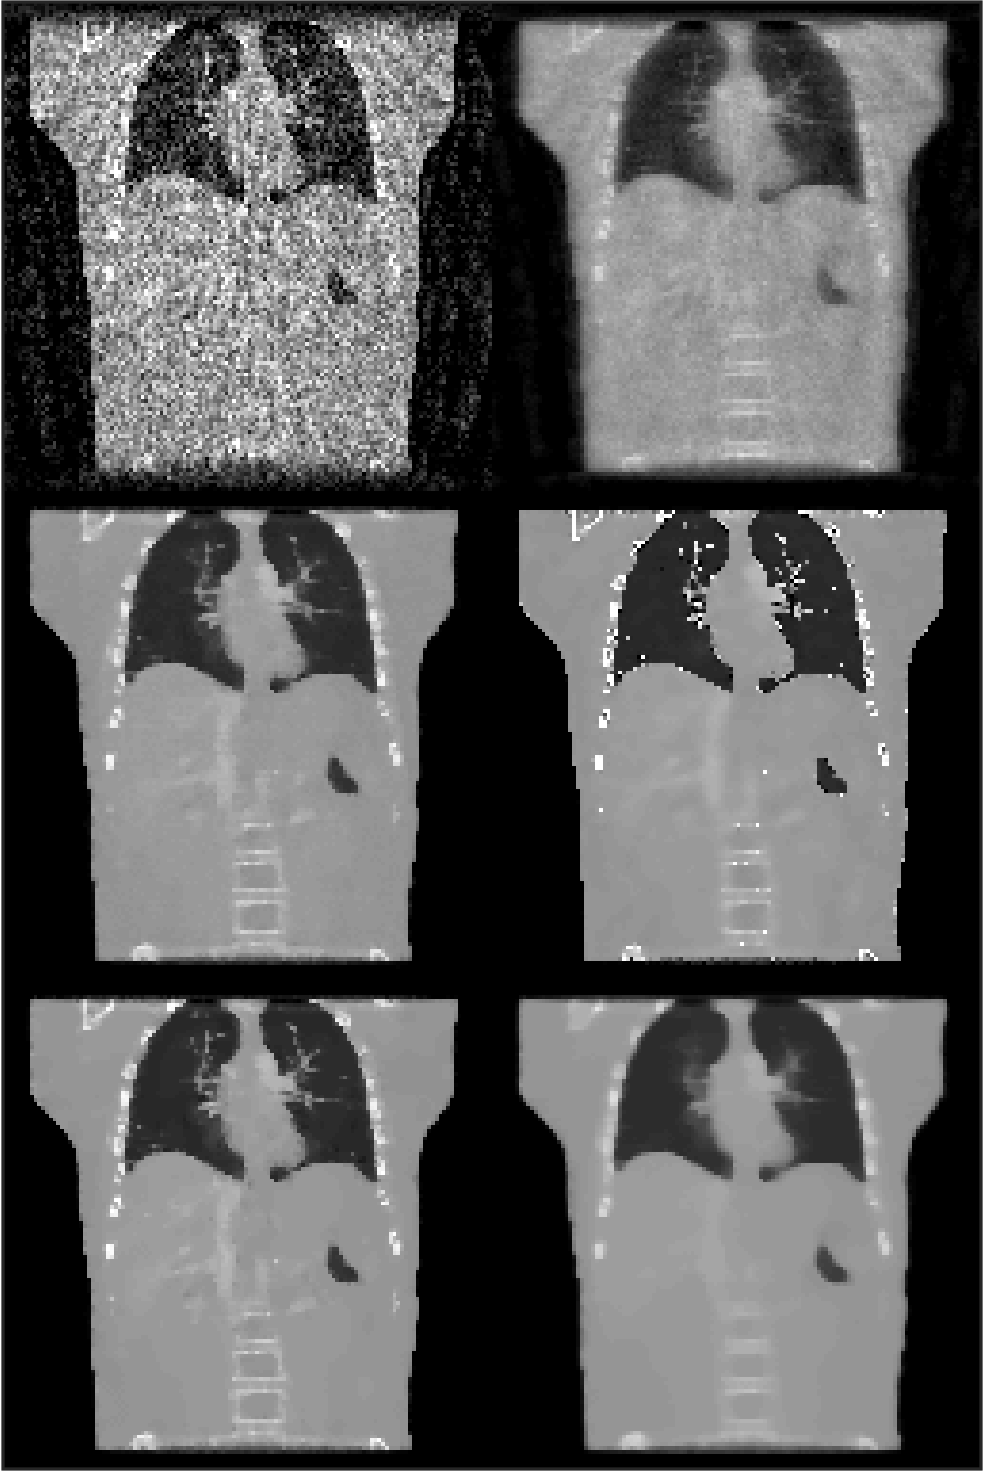
\includegraphics[width=0.4\textwidth]{Applications/TVs2.png} };
\path (B.south west) -- (B.north west) node[pos=.18, above, rotate=90] {ASD-POCS} node[pos=.5, above, rotate=90] {b-ASD-POCS-$\beta$} node[pos=.82, above, rotate=90] {FDK};
\path (B.south east) -- (B.north east) node[pos=.18, below, rotate=90] {OS-ASD-POCS} node[pos=.5, below, rotate=90] {SART-TV} node[pos=.82, below, rotate=90] {OS-SART};

\end{tikzpicture}
\caption[Reconstructed images using TV algorithms]{\label{fig:TVXCAT}Reconstructed images using FDK, OS-SART and the TV algorithms b-ASD-POCS-$\beta$, SART-TV,  ASD-POCS and OS-ASD-POCS with a limited amount and noisy data. Both figures show the same data and algorithms, but with a different cross-section of the image.}
\end{figure}


\begin{table}
\begin{center}
\caption{NRMSE for the reconstructed images in figure \ref{fig:TVXCAT}}
\label{tab:NRMSE TVs}
\scalebox{0.85}{
\begin{tabular}{| l || c | c | c | c | c | c |}
\hline
& FDK & OS-SART &b-ASD-POCS-$\beta$&SART-TV& ASD-POCS& OS-ASD-POCS\\  
\hline
\hline
NRMSE&  0.1373  &  0.0678  &  0.0338   & 0.0267 &   0.0304 &   0.0442\\   

\hline  
\end{tabular}
}
\end{center}
\end{table}






To illustrate the sensitivity to parameter selection, the algorithm SART-TV is run with 3 different values for number of TV-iterations per SART iteration for the same data set used in the previous test. The results can be seen in figure \ref{fig:SARTTVparams}, where one can clearly see how a small changes can have a devastating effect in the output image.   If a few more TV iterations are added to (b), the image gets a bit smoother and some detail is lost, as expected. However, if few iterations are removed from (b), the image can get completely destroyed. Note that these values are only applicable to this image with the exact amount of noise and projections. Different experiments may not show this behaviour or may be more intolerant to parameter change. This is arguably the biggest limitation for the common use of TV algorithms in real application. As an advantageous point, once the good parameters are found, generally the algorithm will perform similarly in similar images, thus application specific parameters may be an option.






\begin{figure}
\centering
\begin{tikzpicture}

\node (A) {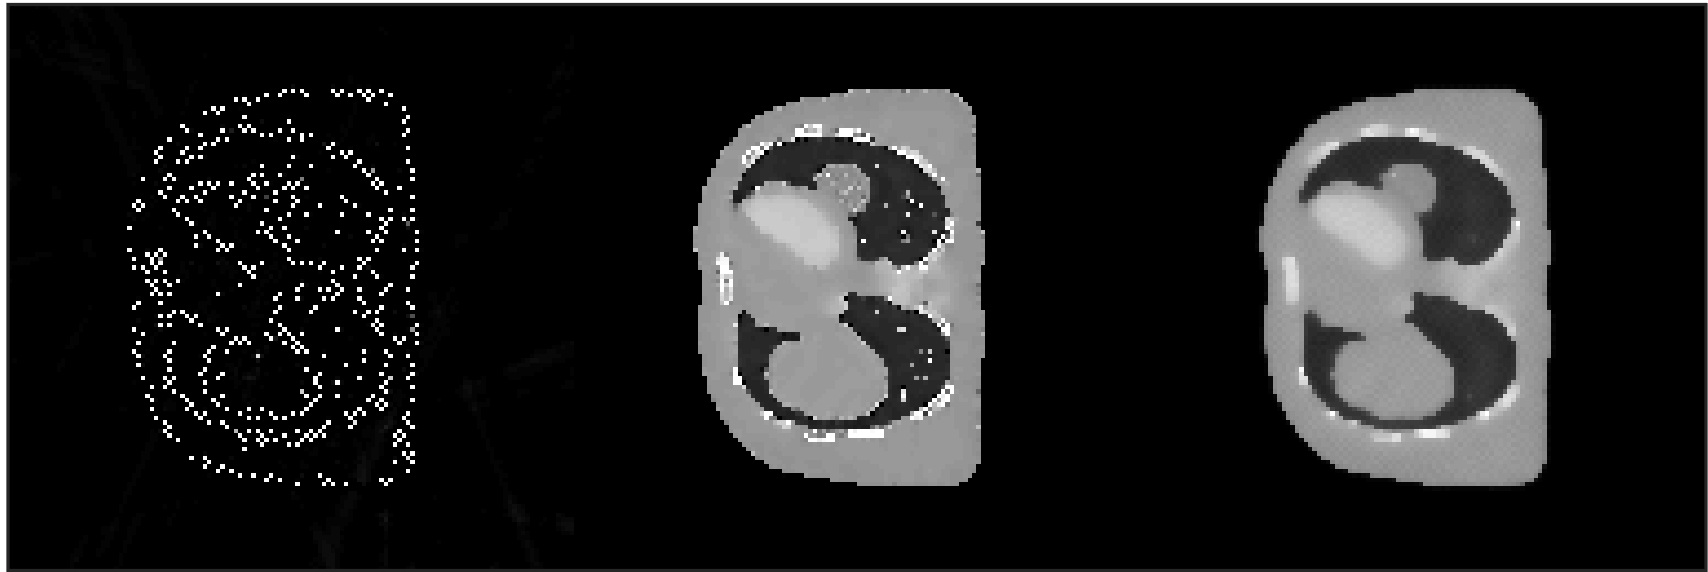
\includegraphics[width=0.7\textwidth]{Applications/TVs3.png} };
%\path (A.south west) -- (A.north west) node[pos=.18, above, rotate=90] {ASD-POCS} node[pos=.5, above, rotate=90] {b-ASD-POCS-$\beta$} node[pos=.82, above, rotate=90] {FDK};
\path (A.south west) -- (A.south east) node[pos=.18, below] {(a)} node[pos=.5, below] {(b)} node[pos=.82, below] {(c)};

\end{tikzpicture}
\caption[SART-TV algorithms with different parameters]{\label{fig:SARTTVparams}SART-TV algorithms with different amount of TV iterations per SART iteration, (a) 32 iterations, (b) 40 iterations, (c) 48 iterations.}
\end{figure}



\FloatBarrier
\section{Iterative Algorithms in Different CT Applications}
This section tries to illustrate the effect of different algorithms within the TIGRE toolbox in a series of datasets. 
\subsection{Medical Head CBCT from  The Christie Hospital}
\subsection{Cryo Soft X-Ray Tomography at Diamond Light Source}

Cryo soft X-ray tomography (Cryo-SXT) is a relatively new[CITE] technology to image micrometer size biological samples in full 3D. Generally, cell-imaging is performed with electron microscopy (EM) machines and all its variants (transmission electron microscopy, scanning electron microscopy, cryo-electron microscopy, electron tomography, etcetera), however these techniques have very limited penetration (less than 1$\mu$m) and thus often require slicing of the samples for volumetric imaging. Cryo-SXT uses the so called water window for X-ray energies around the 500eV energy range. Unlike in higher energies, where everything is invisible, water becomes transparent but carbon-based tissues are clearly visible on that range. Thus, while with lower resolution than most EM, cryooSXT allows for full volumetric visualization of the cells without damaging the samples. In order to be able to image in the extremely accurate setup in both sample handling and X-ray parameters, these cryoSXT images are captured in synchrotron facilities. The data used in this work is from the B24 beam-line at the Diamond Light Source.

However, cryoSXT data has several sources of errors that make its reconstructed images significantly noisy. The typical penetration depth of soft X-rays is around 10$\mu$m, while the samples are generally an order of magnitude bigger than that in height and width. Thus cryoSXT is a limited angle problem, where most of the datasets are sampled over a 120 degrees arc. In the extrema of this range, the images in the detector tend to have little or none information in some parts of the image due to photons not reaching the detector. Additionally, the low intensity and small sample size do mean that there the detector data is very noisy, as photons spread out more (in pixel dimension) and less photons reach the detector. The size of the sample also comes with errors in the mechanical systems of the imaging set up. When working in a scale of microns, any small vibration is visible and considerably offsets/perturbs the measured data. Generally this type of errors are removed by pre-processing using alignment techniques, but the algorithms involved are often not fault proof, and the data used in reconstruction ends up having some misalignment errors. Few of these errors can be seen in the sinogram of the dataset labelled as ``2017\_0207\_Trypanosoma\_33'', on where misalignment and missing data problems are visually perceptible.


Few datasets have been reconstructed from this imaging modality using various algorithms and using various algorithms. Objective evaluation of the quality of the reconstructed image with each algorithm is not possible, as due to the noisy nature of the images, classifying some of the visual artefacts as data or noise is hard. Thus this section does not intend to claim that any of the algorithms perform better than the filtered backprojection (FBP), just highlight the differences.

\subsubsection{The ``2017\_0207\_Trypanosoma\_33'' dataset.} Several algorithms have been used to test the efect of iterative algorithms.
Initially SIRT and CGLS have been chosen. Both of these algorithms are expected to generate images with very few noise, but perhaps lose the most detailed information, or at least create smoother boundaries than FBP, as they minimize the L2 norm using all data in one go (per iteration). Result of these, compared to FBP can be seen in figure \ref{fig:CGLSSIRT}. SIRT generates a very smooth image without barely any noise, however the details are very smoothed also, specially the boundaries of the objects. However, very few iterations of SIRT have been performed in this dataset. More iterations will likely improve the quality of the result, but it is likely that hundreds of them are needed to obtain a good image. CGLS however seemsto separate data from noise better, while also creating some smooth (not as much as SIRT) boundaries. However it is unclear to me how much of this is caused by misalignments on the data and how much by the algorithms themselves.

As shown before in this chapter, OS-SART can improve the convergence speed of SIRT sacrificing some computational time. SART can further this, however as these images are too big, the SART solution would take too long (around 7 hours for 50 iterations). Additionally, total variation minimization can be applied to remove the noise that the images have. Figure \ref{fig:OS} shows FBP, OS-SART, and ASD-POCS with 20 total variation iterations and using OS-SART instead of SART as data fidelity update (OS-ASD-POCS).

Note that the images have a darker vertical ``band'', not as obvious in SIRT and CGLS. This is caused by some errors in the projections that with proper preprocessing step could be removed. OS-SART reconstruct a similar result than FBP, with slightly lower noise levels and extreme values. Les iteration of OS-SART would probably generate a less noisy image, however they will also likely show less contrast and features (similar as SIRT before). The total variation version of OS-SART generates a cleaner image, but it has a slight ``watercolor'' texture. The strength of the total variation can be controlled by the amount of iterations, increasing them enhances this effect. Figure \ref{fig:OStv} shows 0, 20 and 5 TV iterations. While the tuning of this value can not (yet) be done automatically, once the desired one is found it generally works for all similar images. The actual value of the reconstructed voxels is different in each algorithm. This can be explained by the nature of the data, as for example, half of the values are negative, which makes no sense physically. Thus, the visualization range has been tweaked to match histograms in the figures.


\begin{figure}
\begin{center}

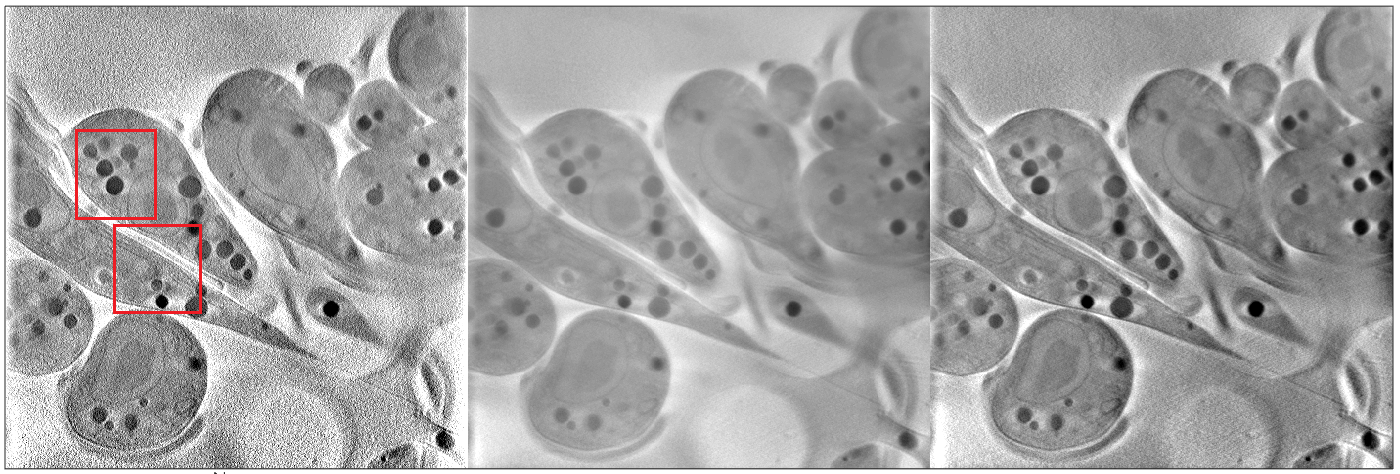
\includegraphics[width=\textwidth]{Applications/FBP_SIRT_CGLSm.png} 
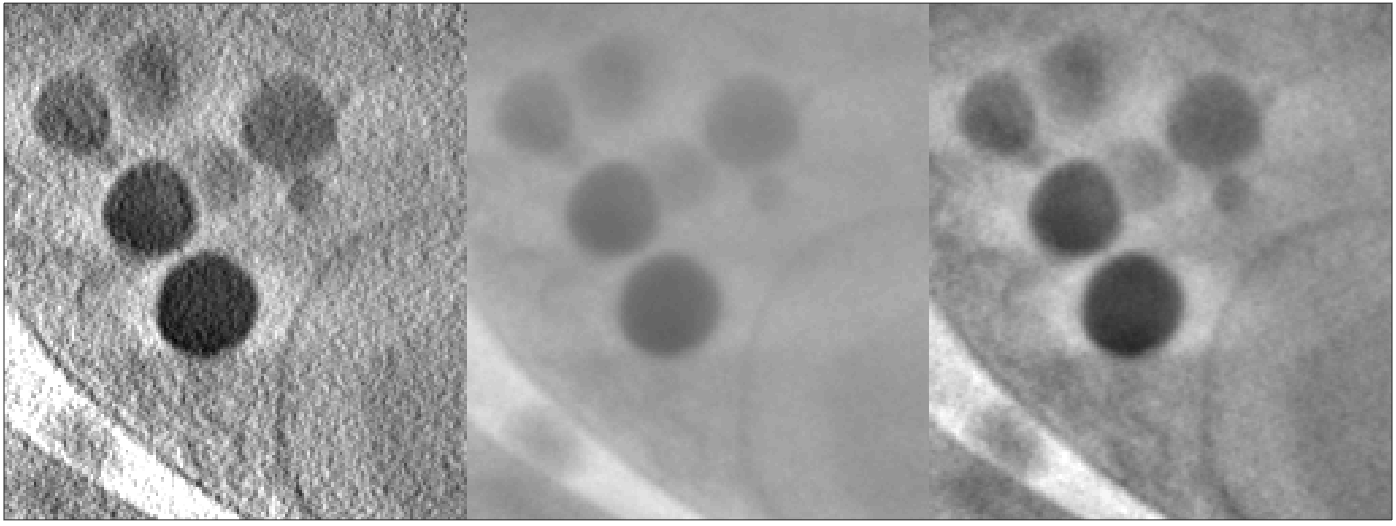
\includegraphics[width=\textwidth]{Applications/FBP_SIRT_CGLSz1.png} 
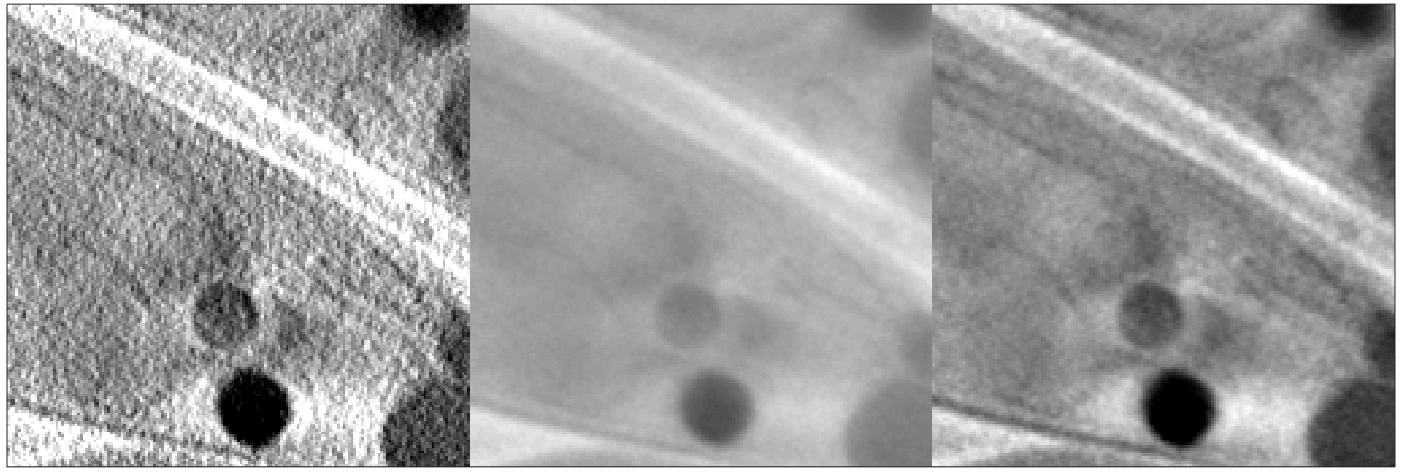
\includegraphics[width=\textwidth]{Applications/FBP_SIRT_CGLSz2.png} 

\end{center}

\caption{\label{fig:CGLSSIRT} Columns: FBP, SIRT (20 iterations) and CGLS (7 iterations)} 
\end{figure}


\begin{figure}
\begin{center}

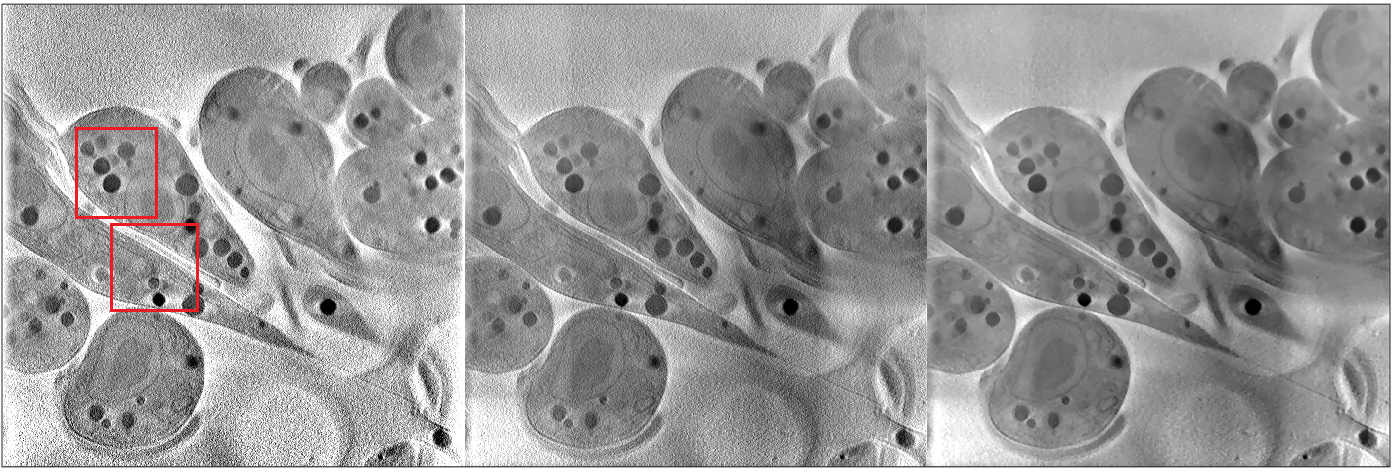
\includegraphics[width=\textwidth]{Applications/FBP_OSSART_TV.png} 
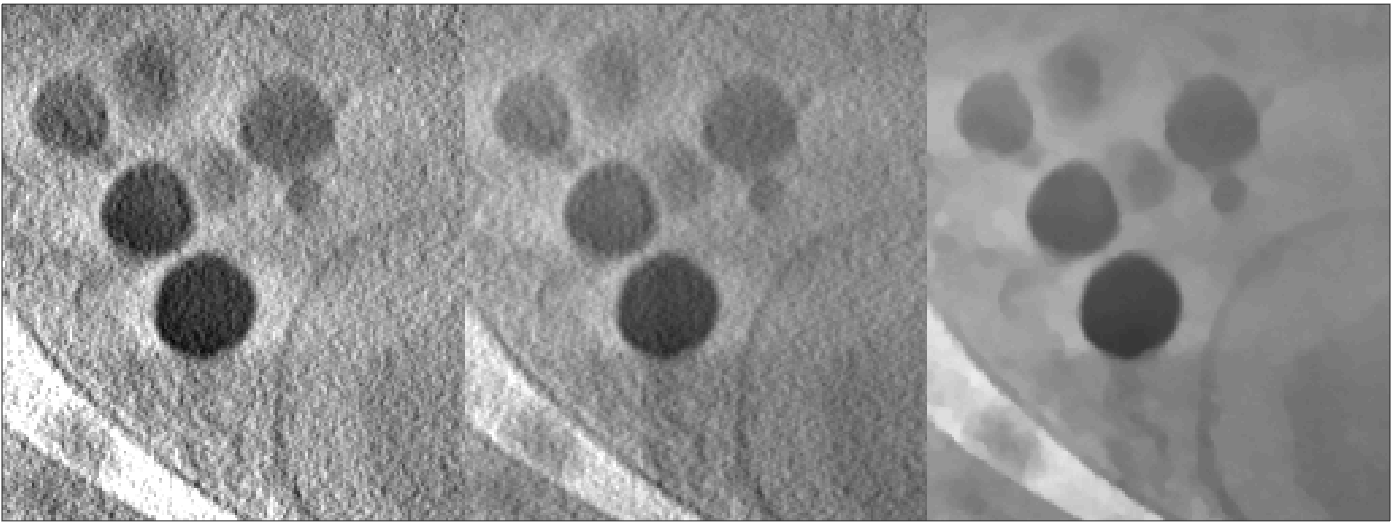
\includegraphics[width=\textwidth]{Applications/FBP_OSSART_TVz1.png} 
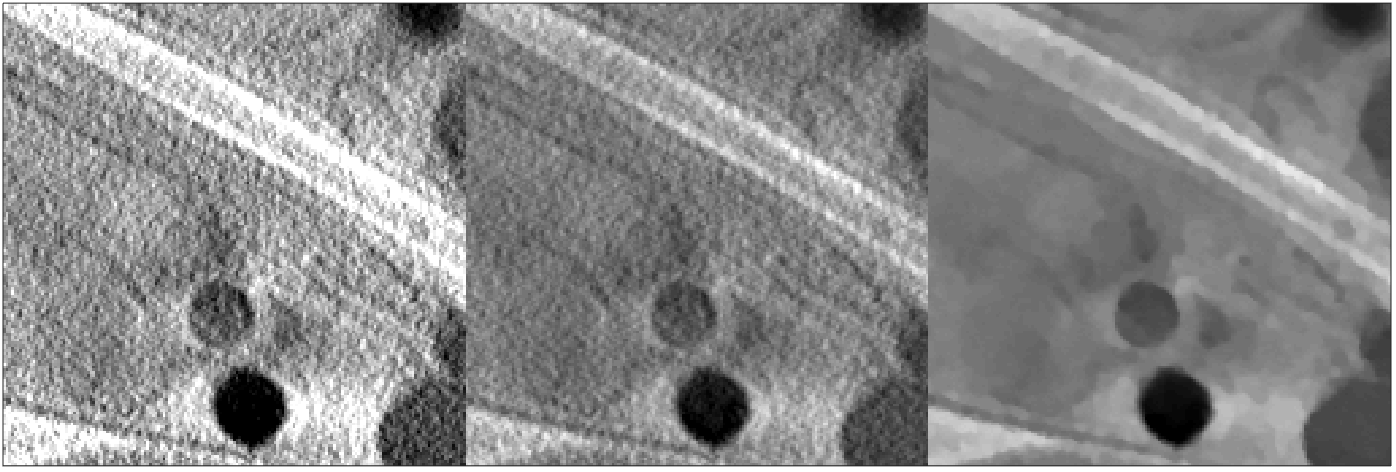
\includegraphics[width=\textwidth]{Applications/FBP_OSSART_TVz2.png} 

\end{center}

\caption{\label{fig:OS}Columns: FBP, OS-SART (20 iterations) and OS-ASD-POCS (20 iterations, 20 TV iterations each)} 
\end{figure}


\begin{figure}
\begin{center}

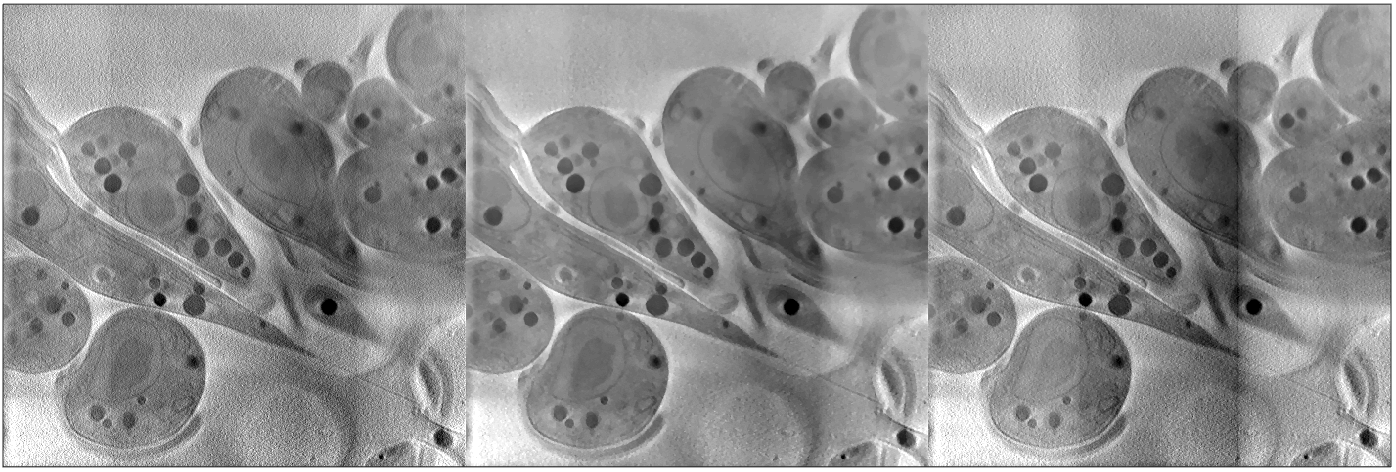
\includegraphics[width=\textwidth]{Applications/OSSART_0_20_5_TViters.png} 
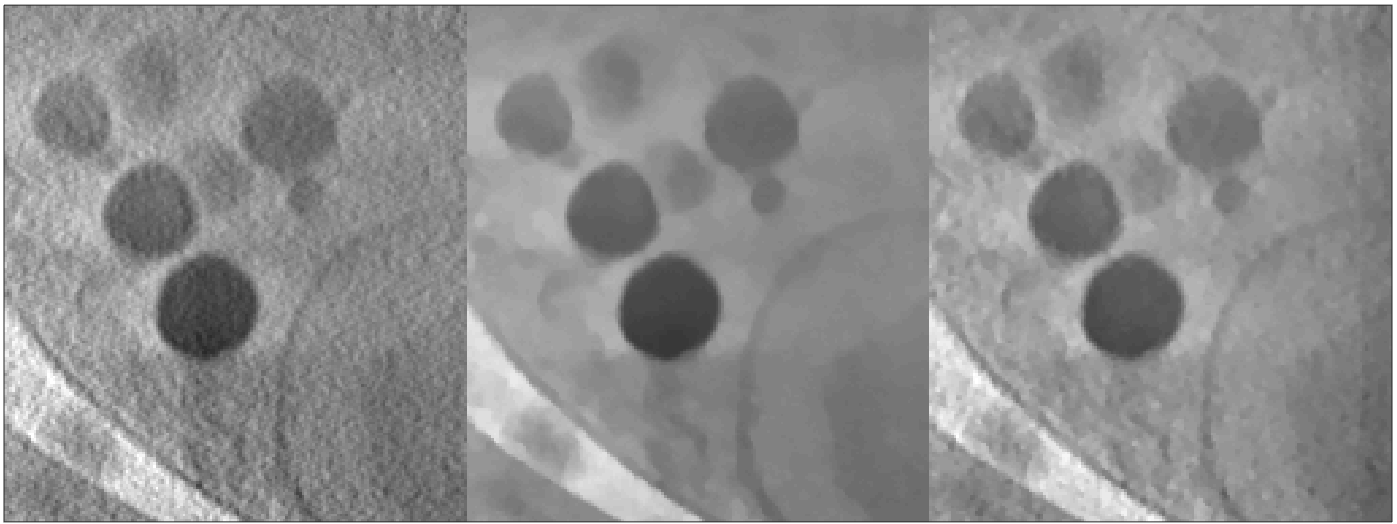
\includegraphics[width=\textwidth]{Applications/OSSART_0_20_5_TVitersz1.png} 
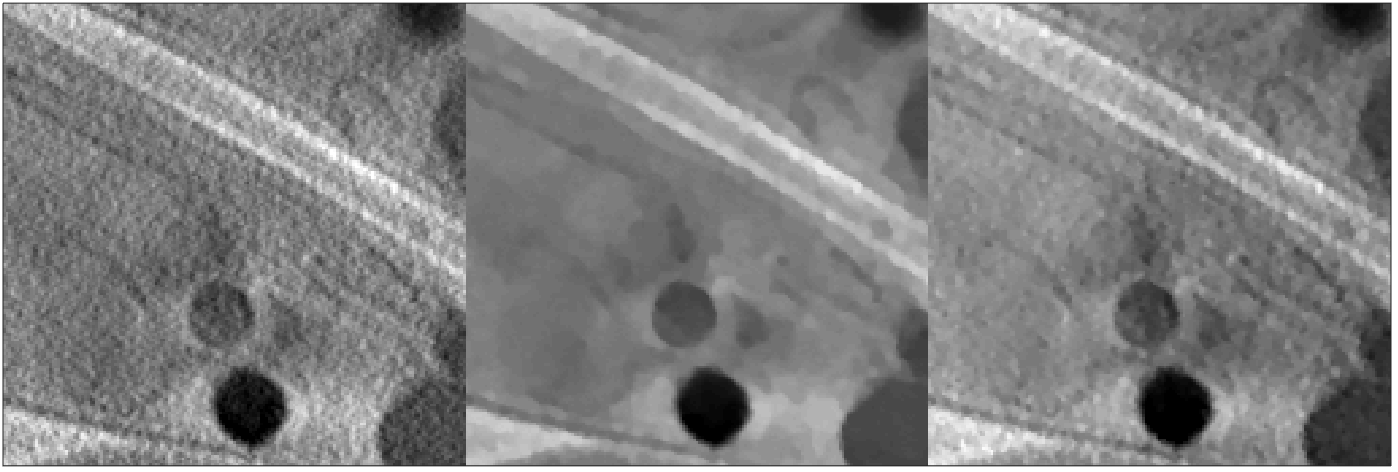
\includegraphics[width=\textwidth]{Applications/OSSART_0_20_5_TVitersz2.png} 

\end{center}

\caption{\label{fig:OStv}Columns: OS-SART (20 iterations, 0 TV iterations), OS-ASD-POCS (20 iterations, 20 TV iterations each), OS-ASD-POCS (20 iterations, 5 TV iterations each)} 
\end{figure}

\FloatBarrier

\subsubsection{The ``3\_20160218\_tomo\_65t55\_p5\_area\_2MB1\_Export'' dataset.}



\begin{figure}
\begin{center}

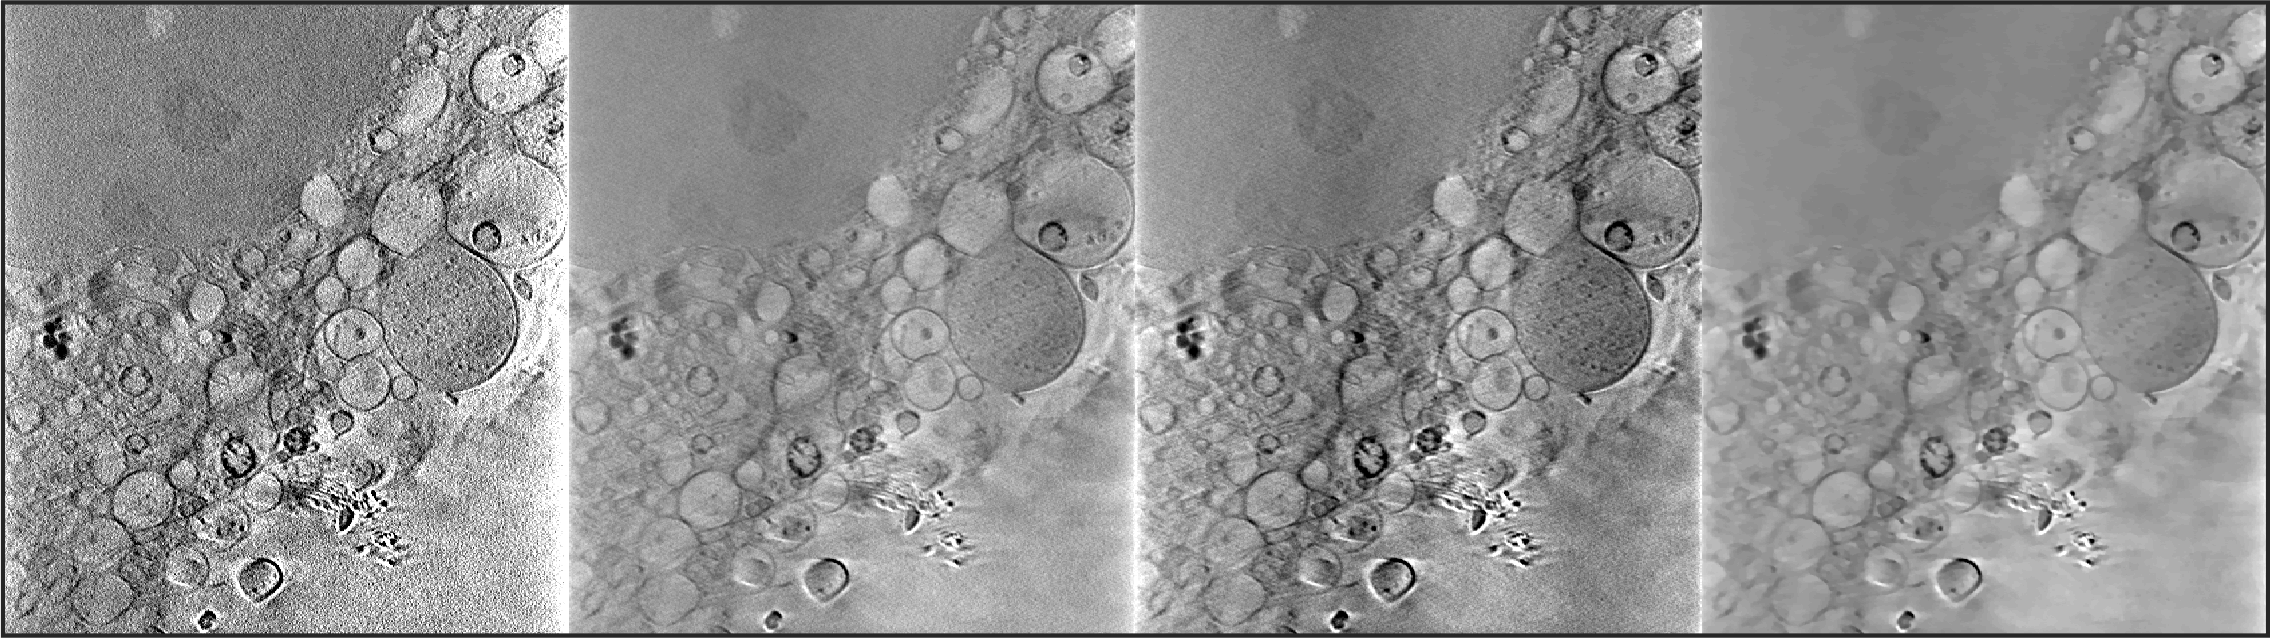
\includegraphics[width=\textwidth]{Applications/Diamond1_full.png} 
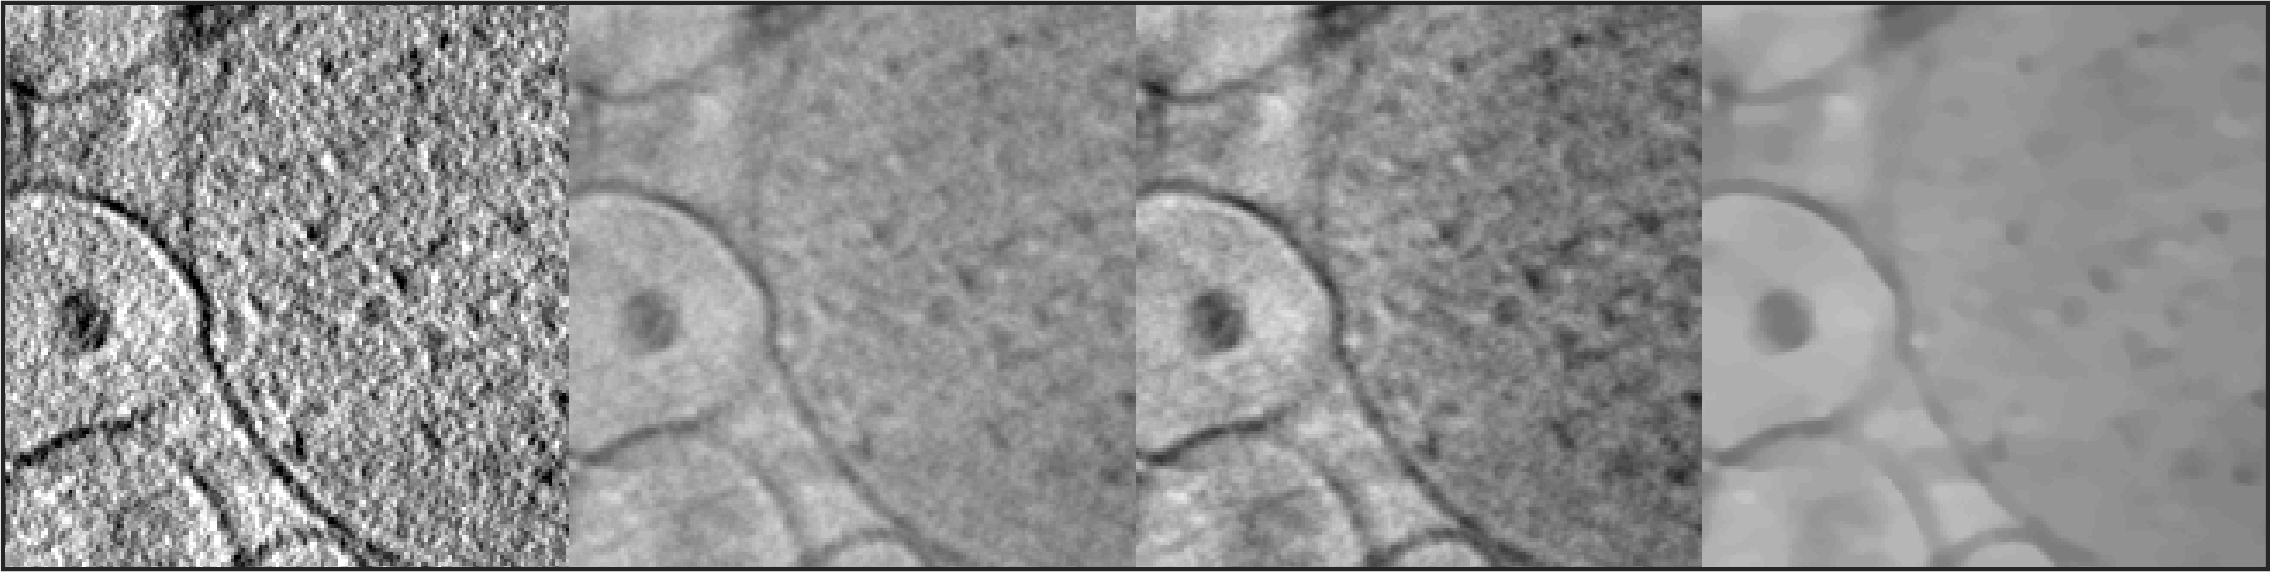
\includegraphics[width=\textwidth]{Applications/Diamond1zoom1.png} 
\includegraphics[width=\textwidth]{Applications/Diamond1zoom2.png} 
\includegraphics[width=\textwidth]{Applications/Diamond1zoom3.png} 

\end{center}

\caption{\label{fig:OStv}Columns: OS-SART (20 iterations, 0 TV iterations), OS-ASD-POCS (20 iterations, 20 TV iterations each), OS-ASD-POCS (20 iterations, 5 TV iterations each)} 
\end{figure}
\label{ch:apllications}

\chapter{Motion compensation modelling}

As broadly discussed in chapter 2, motion is a major source of error in tomographic imaging. The change in location of any image part, or human tissue in the medical field, will effectively be translated into blurring in the reconstruction step. This blurring imposes a big limitation on the possibility of treating cancer in lung and liver, as these are very mobile parts of the body. Having not only accurate spatial information, but also temporal information of these organs can potentially improve the treatment outcome. This means that good 4D imaging techniques can improve radiation therapy. Several methods have been proposed int he literature for compensating for motion in tomography, most of the relaying on the binning of the data into multiple phases. 

In this chapter a completely new approach is introduced and tested based on the ideas developed in the Proton Synchrotron (PS) at CERN for phase space tomography for non-linear motion to medicine. This new method can effectively remove any motion that happened during data acquisition while still using the information of the full dataset to reconstruct the image. This technique, relies in the approximate knowledge of the behaviour of the motion during the scan period and can reconstruct images in any chosen state of the motion.

The chapter introduces the ideas used in the tomography at the PS and explains how can they be transferred to X-ray absorption tomography, using the mathematics and computational techniques presented in previous chapters. First, a description of how to modify the standard GPU techniques and reconstruction algorithms to add the motion compensation is given. Then a series of proofs of principles are given, starting from a very basic motion model and ending using real patient data, using similar techniques than the ones available in a hospital. Finally, an in deep comment of the possibilities of the algorithms is given.

This chapter is widely based on the journal article XXXXXXXXXX.

%Organ movement can be a serious problem in X-ray imaging as the inconsistency between data taken at different phases of the motion leads to blurring and makes the boundaries between different regions hard to distinguish.  This effect is particularly important in image-guided radiation therapy (IGRT), especially for tumours located in the thorax, such as lung or liver tumours.  Respiratory motion is always present and can limit the quality of the image to the point where establishing the precise size, position and boundary of a tumour becomes difficult.  Nowadays the principal clinical solution to ensure the irradiation of all the tumour is to irradiate the entire region where it is estimated to be located during the full respiratory cycle, thus necessarily damaging some healthy tissue.  This is even more critical in hadron therapy because, unlike photons, charged particles deposit most of their energy at the Bragg peak, which means a tumour could be missed completely and only healthy tissue irradiated if targeting is carried out on the basis of inaccurate treatment planning.  Currently one of the most promising real-time imaging technologies is the MRI-Linac, which can acquire some limited image data at a high frame rate.  However, the use of a magnetic resonance imaging (MRI) machine is not compatible with hadron therapy because the magnetic field of the former would perturb the particle beam of the latter.

%The most common device for IGRT imaging is a cone-beam computed tomography (CBCT) machine.  This is a low-dose, low-cost, 3D X-ray modality.  It is used each time a patient undergoes a stage of radiation therapy in order to correct for anatomical changes, such as tumour shrinkage and patient weight loss, that typically occur during the course of treatment.  Due to its lower energy than a conventional CT scan and to its slow data acquisition rate, a CBCT image is generally riddled with noise and motion artefacts.  Research into the removal of motion artefacts in CBCT is widespread and numerous articles have been published on the subject.  The most studied method to deal with motion is phase-correlated CBCT, also called 4D-CBCT\cite{sonke2005respiratory}\cite{thomas2006}\cite{li2006four}\cite{Pengpan2012246}\cite{t2016first}.  In 4D-CBCT, projection data are binned according to respiratory phase and then the data from each bin are reconstructed separately to produce a series of images.  This approach has several drawbacks.  Even though the amount of data per reconstructed image is smaller than usual, the total number of projections increases which means a longer irradiation time and a higher dose for the patient, limiting its clinical use.  In addition, the image quality of each 4D-CBCT reconstruction is inferior to a 3D-CBCT one due to its reduced dataset and to small inconsistencies resulting from binning inaccuracies. 

%Due to the limitations of standard 4D-CBCT imaging, extensive research has been conducted to improve the quality of the images.  This work can be divided into two main groups: algorithmic approaches and deformation vector field (DVF) optimization methods.  Methods in the first group rely on regularization and other similar approaches.  An example is the work by Jia \textit{et al}\cite{jia2012}, who implemented a non-local means of reconstruction to improve the temporal similarity between images.  Total variation methods (TV)\cite{ASD_POCS}, which minimize gradients within an image, have been also proposed with a temporal dimension included in the gradient\cite{0031-9155-57-6-1517}.  Another method based on TV minimization is the so-called PICCS algorithm\cite{chen2008prior}\cite{0031-9155-53-20-006}\cite{chen2012time}, which minimizes the TV and the difference between the reconstructed image and a prior image.  This prior image is generally a CBCT reconstructed with motion artefacts.  PICCS can reconstruct 4D-CBCT images from highly undersampled datasets.  More complex algorithms have also been proposed, such as ROOSTER\cite{:/content/aapm/journal/medphys/41/2/10.1118/1.4860215}, where a series of regularizations and minimizations are performed inside a region of interest to create clear 4D images in that area.

%The methods of the second group generally (but not always) rely on a previous high-quality 4D-CT treatment planning scan as the basis from which to compute the DVFs.  As breathing motion is neither truly periodic nor reproducible in a given patient over time, the DVFs are corrected by matching real projections with simulated ones.  Finally, when the best DVF is computed, a synthetic image is generated by deforming the prior high-quality CT scan.  Examples include the work of Brock \textit{et al}\cite{brock2010} and Ren \textit{et al}\cite{Ren20121584}, who managed to reduce the number of projections required to about 60 using non-linear conjugate-gradient methods.  In order to improve robustness and reduce the dimensionality of the problem, DVF principal component analysis (PCA) methods have also been proposed\cite{zhang2010correction}.  Li \textit{et al}\cite{:/content/aapm/journal/medphys/37/6/10.1118/1.3426002}\cite{:/content/aapm/journal/medphys/38/5/10.1118/1.3582693} demonstrated that good accuracy can be achieved using only a single projection for the DVF optimization.

%Hybrids between DVF-based and algorithmic approaches also exist, such as using TV regularization methods to improve convergence by initializing the DVFs\cite{wang2012high} or using temporal regularization with DVFs to improve the ROOSTER algorithm\cite{mory2016motion}.  Hybrid methods can lead to highly complex optimization strategies.  Examples include segmented mesh-based 4D-CBCT\cite{0031-9155-61-3-996} and the separation of static and moving images using TV, tight frame regularization and DVF optimization\cite{0031-9155-56-11-002}.  In addition, Christoffersen \textit{et al}\cite{christoffersen2013registration} have proposed a multi-step algorithm using TV and optical flow for motion estimation.

%Finally, some special mathematical algorithms have also been suggested that are unique in their approach.  These include the cine-CBCT algorithm\cite{6803058} and the 5D motion modelling approach\cite{0266-5611-31-11-115007}, which does not use phase-correlated binning.

%The literature is made of these and many other approaches, ranging from the computationally and mathematically complex to those that sacrifice accuracy for simplicity and speed.  Most have been shown to yield good 4D-CBCT reconstructions, some in clinical scenarios.  But they all have drawbacks.  CBCT is a severely ill-posed problem where the amount of data is key for a good reconstruction.  The simplest methods that rely on binning will always suffer to some extent from a lack of data, even if temporal coherence is enforced with mathematical norms.  Additionally, they involve the reconstruction of several images, which is very expensive both computationally and in terms of memory.  The DVF-based approaches also have computational limitations.  Those that employ PCA do, indeed, reduce the computational cost by the removal of principal components, but these could describe effects that then are lost.  And most of them ultimately use the DVFs to deform a prior image rather than using the acquired data directly to produce a reconstruction.  Further, they assume that a DVF can describe every possible anatomical change with respect to that prior image and this does not necessarily hold.

%Here, we propose a completely different approach to motion compensation in 4D-CT imaging.  We will focus on thorax CBCT in this article, but the method is generalizable to any X-ray absorption CT modality and to arbitrary motion.  The method requires no binning, but instead uses all projections to reconstruct an image at any respiratory phase.  It does require a sufficiently accurate description of the motion in terms of DVFs, but the approach is a modelling one so it can be used to introduce motion compensation into any iterative reconstruction algorithm. 





%\section{Methods}

%



\section{Alternative motion modelling approach}

Motion in tomography is a problem not only in X-ray modalities.  Phase space tomography \cite{pstweb} is a hybrid algorithm that combines particle tracking in a computer model of a synchrotron with iterative ART to reconstruct an image of the population of a bunch of particles circulating in the accelerator.  The particle motion involves non-linear rotation and is non-cyclic, but a 1D projection of the distribution can be completely acquired as a single snapshot on one turn of the machine.  By tracking test particles to gain a knowledge of how the geometry of the 2D image plane (longitudinal phase space) deforms, the information in all the discrete time slices acquired over many turns can be translated back to the same instant and tomographically combined in a single image.  Conceptually this means adding the motion information to the geometry of the model -- in the $A$ matrix -- with which the problem is posed rather than inserting it somehow into the mathematics of the tomography by which a solution is found.

The concept can be transferred to standard absorption tomography, but the idea of following the motion of test points in a 3D image volume simply does not scale from the 2D tracking used for the modest number of pixels typical in phase space tomography.  It would lead to unreasonable computing times and memory requirements.  Instead, motion is modelled as a different effect with the same mathematical result.  Thus a shift upwards of the voxels in a region of the image is modelled as a local shift downwards of the X-ray paths through a regular voxel mesh that remains frozen in the state at which the reconstruction is made.  The motion can be arbitrary provided it does not send any voxels out of the image or add new ones to it.

The idea is illustrated in figure \ref{fig:motion}, where two different states of motion are sketched.  In order to reconstruct at the initial time (a), the measurement at detector element $d_k$ at later time (b) is back projected along the deformed line of response in (a) and so combined with the measurement at element $d_j$ made directly at the earlier time.  Likewise, if the later time is chosen for the reference state at which to reconstruct, the integral over the deformed line of response in (b) provides the attenuation figure needed to project onto $d_j$ in order to iterate the measurement at that element which was actually made at time (a).  Note that the paths are not only bent (or "warped") but also stretched in some places and compressed in others.

\begin{figure}
\begin{center} 
\subfigure[]{ 
\includegraphics[width=0.45\linewidth]{MotionCorrection/diagrammotion1.pdf} 
\label{fig:fig21a} 
}
\subfigure[]{ 
\includegraphics[width=0.45\linewidth]{MotionCorrection/diagrammotion2.pdf} 
\label{fig:fig21b} 
}
\caption{\label{fig:motion} The integral over a path in image (a) yields the same result as the integral over the same coloured path in the deformed image (b).} 
\end{center} 
\end{figure}



\subsection{Warped projection operator in a GPU}

The warped X-ray paths cannot be easily translated into classic projection operators.  Evaluating the length of a curvilinear path accurately inside every voxel it traverses would require a set of complex numerical methods which would inevitably increase the computation time significantly.  Instead, the uniformly sampled projection method explained in chapter 4 is used, for which the ray-warping operation becomes a straightforward modification of the code.  Rather than sampling at each image coordinate along a straight line, the vector field at that coordinate is first added and then the image is sampled.
 
The pseudocode in a GPU is outlined in algorithm \ref{alg:interp}.  One thread per X-ray is launched to compute $N_{ray}$ threads organized in divV$\times$divU blocks.  This means that instead of computing each of the path integrals in lexicographical order, small subsets of blocks (in the detector) are computed together.  This decreases the memory latency and increases the overall speed of the kernels by up to 300\% in our tests.  For more information about GPU memory access and optimal X-ray indexing we refer the reader to the work by Chou \emph{et al}\cite{Chou2011}.  As information about the texture cache is proprietory, empirical tests were made to find the best size for divV and divU.  These showed 32$\times$32 to be fastest on an NVIDIA Tesla 40k.  Note that there are reportedly faster structures for GPU kernels\cite{forwardproj}, but our tests showed no such improvement so we have stuck to the simplest approach of one thread per ray.

\begin{algorithm}

\caption{Motion interpolated X-ray projection
\label{alg:interp}}
\begin{algorithmic}[1]
\State{Precompute geometric constants}
\Launch{$N_{ray}$ threads organized in divU$\times$divV blocks}
    
\For{X-ray path}
      \State{Compute $[x,y,z]$ sample position}
      \State{Sample $[\textup{DVF}_x,\textup{DVF}_y,\textup{DVF}_z]= \textbf{DVF}(x,y,z)$}
      \State{Sum+= $\Delta l \cdot \textup{Image}(x+\textup{DVF}x,y+\textup{DVF}y,z+\textup{DVF}z)$}      
\EndFor
\EndKernel{} 
\end{algorithmic}

\end{algorithm}

Once an X-ray is selected, it is sampled over its path at every user-provided $\Delta l$ step length.  As previously mentioned, any real-valued coordinates, $p=[x,y,z]$, will yield a sample value using the interpolated read of texture memory.  The point is first sampled over the relevant DVF, yielding the change in coordinates of that specific point, then the image is sampled at the new displaced coordinates, $q=p+\textup{DVF}$.  The DVFs needed are those that describe the deformation from all the shifted states back to the reference one of the reconstruction.   Note that this description must be provided in the coordinate system of the reference state, so that $q-p$ is the extent of the inter-phase motion arriving at $p$ rather than originating from it.  This makes it more complicated than the forward mappings from the reference state to each of the others.



\subsection{Warped back projection operator in a GPU}

Warped back projection is simpler to compute as shown in the pseudocode outlined in algorithm \ref{alg:back}.  First, the standard back projection is computed using memory latency aware voxel ordering.  Then, a second GPU kernel is launched with the same thread and block sizes and, for each voxel, a sample of the relevant shifted image is taken at $(x+\textup{DVF}x,y+\textup{DVF}y,z+\textup{DVF}z)$.  This last step is basically a 3D interpolation.  It is important to note that the DVFs used here are not the same as those for projection.  And, although they are the inverse of each other, that inversion is not nearly as mathematically straightforward as a change of sign.

\begin{algorithm}

\caption{Motion X-ray back projection
\label{alg:back}}
\begin{algorithmic}[1]
\State{Precompute geometric constants}
\Launch{$N_{voxel}$ threads organized in divX$\times$divY$\times$divZ blocks}
    
      \State{Compute $[u,v]$ detector position in line with a source-voxel direction}
      \State{Sample Detector$(u,v)$}
      \State{Compute corresponding weight $w$}
      \State{WarpedImage$ = w *\textup{Detector}(u,v)$}  
      \Ensure{} 
      
      \Require{$N_{voxel}$ threads, organized in divX$\times$divY$\times$divZ blocks}
      \State{Sample $[\textup{DVF}_x,\textup{DVF}_y,\textup{DVF}_z]= \textbf{DVF}(x,y,z)$}
      \State{Image=  $\textup{WarpedImage}(x+\textup{DVF}x,y+\textup{DVF}y,z+\textup{DVF}z)$}      
\EndKernel{} 
\end{algorithmic}

\end{algorithm}

Several reportedly faster back projection operator structures exist in the literature.  We found that the one by Zinsser \textit{et al}\cite{zinsser2013systematic} can lead to execution speeds up to four times faster, but only when multiple back projections are used at the same time in the kernel.  Since the vector fields of the motion-compensated algorithm would generally be different for each back projection, this kernel structure will not acclerate the computation.  However, as the drawbacks of using the more complex structure are negligible, it has nevertheless been implemented in our code.  Thus, if a case is treated in which there is no motion to compensate, it will run more quickly.



\subsection{Motion-compensated algorithm}

Using any iterative CT reconstruction algorithm with warped projection and back projection is simple once the DVFs are known.  But first, a reference image is needed and the DVFs from this reference state to the shifted states must be computed, together with the inverse DVFs back to the reference. Once the DVFs are known, the only modifications to a given algorithm are minor.  Whenever the projection operator is used, the warped projection operator with the inverse DVFs should be used instead.  Likewise, for back projection, the warped version with the forward DVFs should replace the standard code.  This allows motion to be included in both operators inside any algorithm independently of the mathematics that invokes those operators.





\section{Results}

In order to validate the motion-compensation algorithm, two different tests were performed.  The results are presented in this section.  First, a proof of principle is established by subjecting a digital thorax phantom to a well-defined, if somewhat contrived deformation with time.  In this case, the expected image at any instant is perfectly known, but despite this the inverse motion map must still be computed numerically and is necessarily only approximate.  The motion moves all voxels within the image (but not the image boundaries) and the amplitude of the deformation is made substantially larger than any real movement in a breathing patient.  A second test is performed using clinical 4D-CT images, where the motion is only approximately known.  Nevertheless, even an approximate motion model can be exploited to significant beneficial effect.



\subsection{Arbitrary deformation of a digital phantom}

The phantom used is a digital representation\cite{xcatweb} of a human thorax comprising $256^3$ cubic voxels.  Motion is simulated according to equation \ref{eq:motion} using 100 equidistant discrete steps of an arbitrary time scale $t$, which runs from 0 to 1, and using $L=128$.  This creates a steadily increasing sinusoidal deformation in all three spatial dimensions, displacing all voxels throughout the volume of the phantom.  Only the boundaries at the faces of the cube and the three perpendicular mid-planes that intersect at its centre remain unshifted.  Figure \ref{fig:motion_Res2} shows a cross-section of the undeformed reference image at $t=0$ and of the deformed image at $t=1$.  Not only are there no static regions, but the deformation is huge compared with real breathing\cite{Liu2007531}, locally approaching three times that for a typical size of thorax.
\begin{eqnarray}
V(x,y,z) = \bigl(\nonumber\\
8*t*\sin(x \cdot \pi/L)\sin(y \cdot \pi/L)\sin(z \cdot \pi/L),\nonumber \\
8*t*\sin(x \cdot \pi/L)\sin(y \cdot \pi/L)\sin(z \cdot \pi/L),\nonumber\\
8*t*\sin(x \cdot \pi/L)\sin(y \cdot \pi/L)\sin(z \cdot \pi/L)\bigr)
\label{eq:motion}
\end{eqnarray}



\begin{figure}
\begin{center} 
\subfigure[]{ 
\includegraphics[width=0.415\linewidth]{MotionCorrection/thorax8XCAT.png} 
\label{fig:motion_Res2a} 
}
\subfigure[]{ 
\includegraphics[width=0.45\linewidth]{MotionCorrection/thorax1XCAT.png} 
\label{fig:motion_Res2b} 
}
\caption{\label{fig:motion_Res2} Transverse plane of the thorax phantom (a) without deformation and (b) at maximum deformation.  A regular mesh overlay illustrates the motion map, although the actual voxels of the phantom are much smaller than this mesh size. The colour scale is linear attenuation coefficient in the range [0-0.045].} 
\end{center} 
\end{figure}

CBCT data are generated comprising 100 projections, one for each time step and covering a full circle.  In order to benchmark the results, 100 CBCT projections are also generated from the undeformed $t=0$ data alone, providing a comparable dataset for reconstruction but from which motion is entirely absent.  The images are reconstructed using 100 iterations of the SART algorithm.

Figure \ref{fig:result21} shows cuts of three different CBCT reconstructions of the reference state.  Motion is not included in the first and motion compensation is applied only in the last.  The latter reconstruction is qualitatively almost identical to the static one despite the necessarily approximate inverse deformation map.  However, the error in the inverse DVF, which is computed using a kernel splatting technique, is very small with more than 95\% of the errors less than 0.05 voxels in absolute distance.  This is typical of the numerical error that one can expect starting from a forward DVF that is well-known.

The error between the original phantom and each of the reconstructions is shown in figure \ref{fig:error2}.  The image in the uncompensated dynamic case is highly saturated in various places, whereas the motion-compensated image has only slightly higher error overall than the static reconstruction.  One would expect more iterations to reduce the error further.  Cuts in the other planes are found to be qualitatively very similar.

\begin{figure}[ht]
\begin{center}
\includegraphics[width=1\linewidth]{MotionCorrection/motion2XCAT2.png}
\hspace{0.1cm}{\footnotesize (a)}\hspace{4.3cm}{\footnotesize (b)}\hspace{4.3cm}{\footnotesize (c)}
\caption{\label{fig:result21} Transverse cross-section of the CBCT reconstruction made (a) using SART in the absence of motion; (b) with motion using uncompensated SART; (c) with motion using compensated SART. The colour scale is linear attenuation coefficient in the range [0-0.045].} 
\end{center}
\end{figure}

\begin{figure}[ht]
\begin{center}
\includegraphics[width=1\linewidth]{MotionCorrection/motion21errorXCAT2.png}
\hspace{0.1cm}{\footnotesize (a)}\hspace{4.3cm}{\footnotesize (b)}\hspace{4.3cm}{\footnotesize (c)}

\caption{\label{fig:error2} Transverse cross-section of the difference between the known phantom (figure \ref{fig:motion_Res2a}) and the CBCT reconstruction made (a) using SART in the absence of motion; (b) with motion using uncompensated SART; (c) with motion using compensated SART.  The display range is significantly enhanced with respect to that of figure \ref{fig:result21}. The colour scale is linear attenuation coefficient in the range [0-0.01].} 
\end{center}
\end{figure}

Tellingly, the difference between the static reconstruction and the motion compensated one, as shown in figure \ref{fig:error23}, is quasi-uniform with no large differences at the boundaries between tissue types.  This means that, while the error may be larger in the motion-compensated case, it will not prevent the correct delineation of an organ or a tumour.

\begin{figure}[ht]
\begin{center}
\includegraphics[width=0.6\linewidth]{MotionCorrection/motion2errorXCAT2.png} 
\end{center}
\caption{\label{fig:error23} Transverse cross-section of the difference between the static reconstruction of figure \ref{fig:error2}(a) and the motion-compensated one of figure \ref{fig:error2}(c). The colour scale is linear attenuation coefficient in the range [0-0.005].} 
\end{figure}

This test demonstrates that the new method can handle arbitrary, non-cyclic motion and that it works well even when the inverse deformation map is not perfectly known.


\FloatBarrier
\subsection{Real patient data}

The second test is performed using clinical data with precomputed DVFs, which are not entirely accurate.  It is important to note that no real CBCT data are used, only 4D-CT image data.  These are taken from the so-called POPI-model\cite{vandemeulebroucke2007popi} and are publicly available\cite{popi-modelweb}.  The data comprise ten 3D-CT images (labelled from ``0'' to ``9'') of the thorax equally spaced during the breathing cycle of a single patient.  Additionally, motion maps generated by two different methods are provided by the authors describing the inter-phase motion of the voxels.  We choose to use the maps that are generated by the parametric method for no specific reason as, statistically, both methods are reported to have similar errors.  And we choose to use the 3D-CT image labelled ``1'' as the reference state to be reconstructed because the authors provide the motion vectors from this state to all the others.  The reference state of the thorax can be seen in figure \ref{fig:realthorax}.  The particular feature of a tumour is highlighted.

%\begin{figure}[H]
%\begin{center} 
%\includegraphics[width=1\linewidth]{thoraxalmagma.png} 
%\caption{\label{fig:realthorax} 3D-CT scan of a lung radiation therapy patient at breathing phase ``1'' cut to show the tumour (located inside the green rectangle) in the (a) transverse, (b) coronal and (c) sagittal planes.  The colour scale is in arbitrary units.} 
%\end{center} 
%\end{figure}



% NOTE TO EDITOR: I tried to make the spacing between figures the smallest, but the
\begin{figure}[H]
\begin{center}
\hspace*{\fill} 
\subfigure[]{ 
\includegraphics[scale=.2]{MotionCorrection/thoraxmagma_1.png} 
}\hfill
\subfigure[]{ 
\includegraphics[scale=.2]{MotionCorrection/thoraxmagma_2.png} 
}\hfill
\subfigure[]{ 
\includegraphics[scale=.2]{MotionCorrection/thoraxmagma_3.png} 
}\hfill
\hspace*{\fill} 

\caption{\label{fig:realthorax} 3D-CT scan of a lung radiation therapy patient at breathing phase ``1'' cut to show the tumour (located inside the green rectangle) in the (a) transverse, (b) coronal and (c) sagittal planes.  The colour scale is linear attenuation coefficient in the range [0-2000].} 
\end{center} 
\end{figure}



In order to simulate CBCT data, projections are generated from the phase-binned 3D-CT images.  No extra noise is added as the images themselves are already noisy.  \textcolor{black}{One hundred equally spaced projections covering a full circle are generated for each of the ten states and from these a subset is chosen, 10 from each breathing phase, to give 100 projections each 3.6 degrees apart and spanning a complete breathing cycle.}  Note that the DVFs are not used to approximate continuous movement as this would compromise the independence of the test that the quality of any subsequent motion-compensated reconstruction employing those DVFs affords.  In order to benchmark the results, 100 CBCT projections are simulated from the state ``1'' data alone, providing a comparable dataset for reconstruction but from which motion is essentially absent.

There are four significant error sources inherent in the original 4D-CT data before a CBCT reconstruction is even attempted.  There is that due to phase binning, which is particularly significant in the regions that move the most.  This is visible in figure \ref{fig:realthorax}, for example in the lower boundary of the lungs.  Another error source lies at the top and bottom (in the cranial-caudal direction) of the 3D-CT images.  Due to the original data acquisition and reconstruction techniques, the images have increased noise-like errors in their extrema and, because of the randomness of these errors, the images are not entirely consistent with each other in these regions.  The third main error in the source data is the inaccuracy of the DVFs in some areas.  Finally, the inverse of the DVFs will have additional errors due to the numerical method used to invert them.

Given these numerous sources of error, one can expect streak artifacts in addition to the usual random noise exhibited in any reconstruction.  As previously mentioned, it is a strength of the new motion-compensation method that it can be applied to any iterative algorithm, so one can be employed that reduces such artifacts by, for example, minimizing the total variation (TV).  We elect to use both the well-known SART and the TV algorithm ASD-POCS\cite{ASD_POCS} in this test.

Figure \ref{fig:res3} shows cuts of four different CBCT reconstructions of the reference state.  Motion is included in all except the first, but motion compensation is applied in only the last two.  The SART algorithm is used in all cases except the last, which is processed with ASD-POCS.  The second, uncompensated image has lost much of the detail inside the lungs, while the compensated algorithms, even with all the errors in the DVFs and data, reconstruct the tissue boundaries inside the thorax with higher accuracy.  The last, TV case is particularly good.  This is even more evident in figure \ref{fig:res3err}, where the difference between the original 3D-CT image and each reconstruction is shown.  One can see that the error is smaller overall in the motion-compensated cases, for which the discrepancy where the tumour is located is barely visible.  Cuts in the coronal plane, which is the one containing the largest movement of the lungs, underscore the remarkable improvement in the motion-compensated images (see figures \ref{fig:tumourCC} and \ref{fig:tumourCC_err}).

\begin{figure}[H]
\begin{center} 

\includegraphics[width=1\linewidth]{MotionCorrection/res32.png} 
\hspace{0.1cm}{\footnotesize (a)}\hspace{3.2cm}{\footnotesize (b)}\hspace{3.2cm}{\footnotesize (c)}\hspace{3.2cm}{\footnotesize (d)}

\caption{\label{fig:res3}  Transverse cross-section of the CBCT reconstruction made (a) using SART in the absence of motion; (b) with motion using uncompensated SART; (c) with motion using compensated SART; (d) with motion using compensated ASD-POCS. The colour scale is linear attenuation coefficient in the range [0-2000].} 
\end{center} 
\end{figure}

\begin{figure}[H]
\begin{center} 
\includegraphics[width=1\linewidth]{MotionCorrection/res3err2.png} 
\hspace{0.1cm}{\footnotesize (a)}\hspace{3.2cm}{\footnotesize (b)}\hspace{3.2cm}{\footnotesize (c)}\hspace{3.2cm}{\footnotesize (d)}
\caption{\label{fig:res3err}  Transverse cross-section of the difference  between the original 3D-CT image (figure \ref{fig:realthorax}(a)) and the CBCT reconstruction made (a) using SART in the absence of motion; (b) with motion using uncompensated SART; (c) with motion using compensated SART; (d) with motion using compensated ASD-POCS. The colour scale is linear attenuation coefficient in the range [0-400].} 
\end{center} 
\end{figure}

\begin{figure}[H]
\begin{center} 
\includegraphics[width=1\linewidth]{MotionCorrection/tumourCC2.png}
\hspace{0.1cm}{\footnotesize (a)}\hspace{3.2cm}{\footnotesize (b)}\hspace{3.2cm}{\footnotesize (c)}\hspace{3.2cm}{\footnotesize (d)} 
\caption{\label{fig:tumourCC}  Zoom on the region where the tumour is located in a coronal cross-section of the CBCT reconstruction made (a) using SART in the absence of motion; (b) with motion using uncompensated SART; (c) with motion using compensated SART; (d) with motion using compensated ASD-POCS. The colour scale is linear attenuation coefficient in the range [0-2000].} 
\end{center} 
\end{figure}

\begin{figure}[H]
\begin{center} 
\includegraphics[width=1\linewidth]{MotionCorrection/tumourCC_err2.png}
\hspace{0.1cm}{\footnotesize (a)}\hspace{3.2cm}{\footnotesize (b)}\hspace{3.2cm}{\footnotesize (c)}\hspace{3.2cm}{\footnotesize (d)} 
\caption{\label{fig:tumourCC_err}  Zoom on the region where the tumour is located in a coronal cross-section of the difference  between the original 3D-CT image (figure \ref{fig:realthorax}) and the CBCT reconstruction made (a) using SART in the absence of motion; (b) with motion using uncompensated SART; (c) with motion using compensated SART; (d) with motion using compensated ASD-POCS. The colour scale is linear attenuation coefficient in the range [0-400].} 
\end{center} 
\end{figure}


For a more quantitative assessment, the resultant images are cropped around the tumour taking a 36$\times$36$\times$26 subset of voxels in the anterior-posterior, lateral and cranial-caudal directions (as indicated by the green rectangles in figure \ref{fig:realthorax}).  Then, in order to evaluate the quality of the reconstruction inside this box, three different indices are used to compare the original 3D-CT image with the four CBCT reconstructions of this test.

\begin{itemize}

\item Root Mean Square Error (RMSE) is defined
\begin{equation}
\boldsymbol{\textrm{RMSE}}=\sqrt{\frac{\sum_{n=1}^N(\hat{p}_n-p_n)^2}{N}},
\end{equation}
where $\hat{p}_n$ is a voxel in the original image, $p_n$ a voxel in the reconstructed one and $N$ is the number of voxels.  A larger value means more difference.

\item Universal Quality Image (UQI)\cite{wang2002universal} is a widely used index and is defined
\begin{equation}
\boldsymbol{\textrm{UQI}}=\frac{2\textrm{cov}(\hat{\mu},\mu)}{\hat{\sigma}^2+\sigma^2}\cdot \frac{2\hat{\mu}\mu}{\hat{\mu}^2+\mu^2},
\end{equation}
where $\textrm{cov}$ is the covariance function and $\hat{\mu},\mu$ are the means and $\hat{\sigma}^2,\sigma^2$ the variances of the original and reconstructed images, respectively.  UQI yields a value between 0 and 1, increasing with increasing similarity.

\item Segmentation mismatch.  A segmentation value using Otsu's method\cite{otsu1975threshold} is computed for the original image and all voxels in the reconstructed image are identified as lying inside or outside the tumour according to that value.  Then the number of voxels that are mislabelled by that segmentation is counted.  A larger value means more difference.

\end{itemize}

The results for each index applied to the subset of voxels in the region of the tumour is shown in table \ref{tab:quality}.  As expected, the SART reconstruction even in the absence of motion in the data does not reproduce the original image with any great accuracy as the data are still not perfect and CBCT reconstruction has its limitations.  Nevertheless, it is a sufficiently good reconstruction to take as a benchmark for the others.  Indeed, it should be stressed that, although the CBCT data here are artificial, in a practical scenario the equivalent static dataset would require a full order of magnitude more radiation dose to acquire than the dynamic one because of phase binning.  In comparison with this static CBCT case, uncompensated SART applied to the dynamic data has considerably worse reconstruction quality, missing almost 10\% of the tumour by segmentation.  Motion-compensated SART performs significantly better, getting closer to the static SART values.  Finally, the motion-compensated ASD-POCS results are very similar to those of the reconstruction without any motion.  One would expect more advanced TV algorithms to perform even better.
  
\begin{table}[H]
\begin{center}
\caption{Tumour reconstruction quality by different algorithms}
\label{tab:quality}
\begin{tabular}{|l|| c | c | c |}
\hline
 & RMSE & UQI & Seg. mismatch \\
\hline \hline  
 SART without motion & 67.18 & 0.9656 & 1108 (3.288\%)\\
 SART with motion & 172.12 & 0.7617 & 3315 (9.838\%)\\
 SART motion-compensated & 109.84 & 0.9077 & 1505 (4.466\%)\\
 ASD-POCS motion-compensated & 82.72 & 0.9451 & 1284 (3.811\%)\\
\hline  
\end{tabular}
\end{center}
\end{table}

This test demonstrates that the new method can be used in a clinical context even if the motion due to breathing is only approximately known.



\subsection{Computation times}
\textcolor{black}{An important factor for clinical feasibility is the computation time that motion compensation adds to a standard reconstruction. The kernel times have been measured on a TESLA k40 GPU and are reported for the projection and back projection operations both with and without motion compensation. Two variants of the back projection operation have been tested, the single- and the dual-kernel versions as described in algorithm \ref{alg:back}. Table \ref{tab:times} lists computation times for $512\times 512 \times 141$ image and DVF sizes and a $512^2$ detector size. The reported times are the average of 100 calls and only account for kernel time. As the back projection kernels are optimized for multiple calls, the average computation times for a single update or a multiple update are different. Both these times are shown in the back projection columns of Table \ref{tab:times}. Reducing the size of the DVFs hardly changes the computation time as the number of samples needed is determined by the image size alone.}

\textcolor{black}{Both the single- and dual-kernel back projection operations lead to similar reconstructed image quality, with a visually imperceptible improvement in the dual-kernel case (0.1 in RMSE). The dual-kernel approach is expected to be better as errors in the DVFs are amplified by the divergent cone angle in the single-kernal case.}

\begin{table}[H]
\begin{center}
\caption{GPU kernel times per projection.}
\label{tab:times}
\begin{tabular}{|l|| c | c | c |}
\hline
& Projection & \thead{Single-kernel \\Backprojection} & \thead{Dual-kernel\\ Backprojection}\\  
\hline
\hline
Standard& 6.5ms& 4ms/2.5ms&-\\   
Motion warped&120ms &24ms/18ms &13ms/3ms\\
\hline  
\end{tabular}
\end{center}
\end{table}

\section{Discussion}

We have demonstrated a significant improvement in CBCT image quality by removing motion artifacts using a modelling approach to motion compensation.  The resultant images still have some error compared with a static reconstruction, but critically, tissue boundaries are resolved with much greater accuracy than when motion is ignored. 

One of the greatest strengths of the new method is that it employs all the projection data to reconstruct an image, reducing the X-ray dose to the patient.  It is also completely algorithm independent; its novelty lies in a modelling approach, which in principle can be applied in conjunction with any static reconstruction algorithm.  In fact, most of the motion-compensation ideas present in the literature and reviewed at the beginning of this work could incorporate the method.  As some of these rely on refining DVFs, then, instead of using those DVFs to generate a deformed image from a prior high-quality one, they could be used to reconstruct images from the real acquired data.  Others rely on temporal reconstruction constraints, where the images at successive time steps are regularized to look similar to their neighbours.  Again, such techniques can be used in combination with the new motion compensation because the latter permits any state of the motion to be reconstructed.  Indeed, one could generate an X-ray video of the patient breathing if enough time steps are reconstructed and, as these frames are computationally independent, they could be processed in parallel.  And none of these extra images would require any extra dose for the patient.

The use of DVFs can lead to large memory requirements and an increased preprocessing time, but it has been established in phase space tomography that it is possible to trade off the accuracy of the maps against an increased number of iterations and that some parameters in the motion model itself can be refined by their influence on convergence\cite{pst1}\cite{pst2}.  More speculative is the idea of "bootstrapping" the DVFs without starting from any high-resolution images.  One can imagine repeatedly subdividing the CBCT data into more and more motion phases, and thus iterating both the images and the DVFs themselves at each subdivision, whilst still using all the data for each reconstruction by interpolating between DVFs until there are enough of these to describe the motion in sufficient detail.  This would be very heavy computationally and there is no guarantee of convergence.

As presented here, the method takes only 2 to 3 times longer than a standard iterative reconstruction algorithm due to the use of GPUs for the motion-compensated projection and back projection operators.  So the computational penalty is not large.  It is important to note that we used DVFs of the same size as the images (they are generally smaller) and the code was not highly optimized.  Careful tuning should lead to appreciably faster execution.

\textcolor{black}{One drawback of the method in an eventual clinical scenario is the need for a sufficiently accurate DVF for each of the projections. Obtaining realistic patient-specific DVFs is non-trivial.  However, statistical analysis\cite{Sonke2008590}\cite{0031-9155-51-17-003} has shown that, while inter-patient motion variability is high, intra-patient variability is low provided the patient performs free breathing.  And preliminary tests of DVF error tolerance of the motion compensation method suggest that the algorithm is very robust to undersampled and noisy DVFs due to its iterative nature, but futher study is required.  Additionally, a method that maximizes the quality of the DVFs needs to be identified. Obtaining the breathing amplitude using the Amsterdam Shroud\cite{0031-9155-58-5-1447} and correlating that with prior DVFs or with DVFs obtained using binned, low-resolution 4D-CBCT images from the same dataset are promising techniques.}

We consider that this motion compensation method could have a genuine impact in IGRT even though it is not yet at a clinical stage.  Better diagnostic imaging offers the prospect of less collateral damage to healthy tissue and increased survival rates.  Ultimately, it might be possible to steer a particle therapy beam in real time to follow a moving target. 



	
%\section{Conclusions}
%A novel approach to motion-compensated CT imaging has been demonstrated that uses the entire dynamic set of acquired data to reconstruct an image that is effectively rendered static, thereby considerably reducing motion artefacts.  This introduces the possibility of a significant reduction in radiation dose during imaging and treatment.  The method requires a knowledge of the deformation vector fields describing the motion between the reconstructed state and all others during the acquisition time span.  It removes much of the unwanted artefacts due to motion even when that knowledge is imperfect.  The method can be used in combination with most, if not all, existing static and 4D iterative reconstruction techniques.  Motion compensation based on these ideas is being rolled out to the algorithms available from the open-source TIGRE Toolbox\cite{TIGREweb}.  The potential clinical benefits are clear.



%\section{Acknowledgements}
%The authors would like to thank EPSRC for helping to fund this PhD work and NVIDIA for the hardware donation of a GPU.  Special thanks go to Robert Bryll and Imanol Luengo for interesting discussions and for speeding up the GPU code.

\chapter{Numerical Study of Motion Compensation}


In the previous chapter of this thesis a motion compensation algorithm is proposed as a general algorithm, and then is specifically focused for IGRT. The method however is scarcely compared with standard IGRT 4D CBCT image reconstruction methods, and some questions about the reliability of the motion models arise. Obtaining accurate motion description of the patients is still one of the biggest challenges in 4D imaging, regardless of the method used. How accurate do this models need to be? Additionally, if the motion is previously known to high accuracy, is 4D imaging necessary at all? 

This chapter looks more specifically at these challenges and compares the motion compensated reconstruction to \label{ch:motion analisis}
\chapter{Conclusions and future work}

The work presented in this thesis can be broken down into two main parts, the TIGRE Toolbox, and the motion compensation modelling technique. Extensive discussion of both has been presented in each chapter of this document, and a more general approach is taken here. 

The TIGRE Toolbox is an easy to use and fast toolbox that provides a wide variety of iterative algorithms to anyone to test. The toolbox is easy to use for both general tomography users or researchers in algorithms, as it has a highly modular design, allowing every algorithm to be used without nothing more than a simple geometry description of the machine and the data, but also having modular blocks for the projection and backprojection operators (with different modes in each) for algorithm researchers to both explore the current algorithms in TIGRE and to implement new ones without worrying about the computationally expensive parts. 

The algorithms implemented in TIGRE are not necessarily the best algorithms nor necessarily representative of all algorithms in CT, however they are a subset of commonly known algorithms, from SART types that have been in CT since the first scan, to later additions to the field such as CGLS or ASD-POCS, they are algorithms commonly seen in the literature. However, the author highly encourages any reader to submit their implementation of new or existing algorithms to TIGRE. The more algorithms that TIGRE have implemented, the better for researchers to explore.

Computationally speaking, the linearised fast projection and backprojection methods implemented are within the fastest published methods for GPU X-ray tomography and experimentally reach very high speeds. The fact that the toolbox is an interface between the a high-level programming language and a low level one, however, reduces the overall computational speeds of algorithms, specially with single projection update algorithms, such as SART or ASD-POCS. Most of TIGRE could be speeded up by implementing the entire algorithms directly in C++/CUDA and never using a high level language such as MATLAB or Python, however the innovation process of writing new algorithms would be significantly crippled, as one can expect an order of magnitude more lines of code when writing the same code in C++ instead of MATLAB. The take-home message is that TIGRE is not the fastest possible iterative reconstruction toolbox as its focused for applied research use, not designed as a final product. However, most of the algorithms can be re-coded into reconstructions within minutes using the correct approaches and hardware. The GPU kernels, however, are already highly optimized, so less work would be needed in this part.

Possibly one of the most important results of TIGRE and its iterative algorithms is the possibility of the wider applications outside lung IGRT. The variety of iterative algorithms allow users to tailor reconstruction for specific applications, as metrology, medical imaging, scientific imaging and industrial quality control (among other applications) have all very different requirements for what is ``good quality''. For example in lung IGRT and in metrology, boundaries between objects are the most important features, while in quality control or in some scientific applications (such as material sciences) small details may be what the user is looking for. Analytic algorithms such as FDK are generic, but can not be tailored to specific requirements. Due to the modular design and flexibility of TIGRE, it can be use in any application directly.


The GPU accelerated motion compensation method presented can, without any data binning, reconstruct a static image in any breathing phase using prior approximated information from the expected motion. The work here shows that if the motion is perfectly known, the reconstruction is nearly equal to a 3D static reconstruction, with minimal interpolation-caused error. The work presented in this thesis also numerically studies the effect of the most common errors in DVFs in the algorithm, showing that it has minimal impact in the reconstructed images. Also it is important to note that as the proposed CPU-based motion compensation is applied to the basic building blocks of the iterative reconstruction, any existing (and possibly, future) iterative algorithm can be used together with the motion modelling method to reconstruct static images, as it is shown with SART and ASD-POCS. 

This thesis shows the potential that motion compensation and iterative algorithms can have in IGRT and particularly in hadron therapy. And making all available code and algorithms public paves the way for further test with clinical data, hopefully bringing adaptive RT therapy closer to an every day treatment for lung cancer patients.


\section{Future work}

As it is common with research work, the future work possibilities span a wider and longer research focus than the work itself. From the two main research items presented  in this thesis (TIGRE and motion compensation), the future work diverges.

The TIGRE toolbox can be enhanced in multiple ways. The toolbox itself lacks X-ray based Input/Output functions (e.g. reading Nikkon, or DIDCOM data and writting in ``vol'' or other formats) that would make the software considerably more approachable for users that only want to experiment with the code. The range of iterative algorithms is a clear place to enhance the toolbox, specially in Krylov subspace methods and statistical methods. The former because the algorithms converge very fast comparing to classic methods, the later because there are no algorithms of that type in TIGRE and it would benefit from a new iterative approach than the currently present. Certainly any addition on algorithms, pre or post processing techniques can be part of future work.

In the more computational side, implementing a matched backprojection would be the next step. Algorithms like CGLS (Krylov subspace algorithms) are greatly affected by having only a partially matched backprojection, and while each iteration would be slower with it, a more robust usage of these algorithms would be possible, thus making the global reconstruction times faster. In the GPU methods side, there are few possibilities that are mentioned in Chapter 4 for exploring acceleration of the projection operator, but results may not be as good as presented in the literature. Finally, the computational side would benefit greatly from multi-GPU support of TIGRE. At the time of writing of this thesis, a multi-GPU branch is available in GitHub (thanks to R.B.), but still not fully integrated in TIGRE.

In the software engineering side, TIGRE would benefit from a clear thing: being totally free. As from the time of this thesis, TIGRE's full potential can be only used with the MATLAB software, and a less complete Python version is available. Making TIGRE fully available for in Python would make the toolbox available for an even wider audience. We encourage users to contribute to the Python version.

The GPU-based motion compensation method has a different, yet clear future work. The method has been shown working to high robustness and image reconstruction quality using synthetic data, the next step would be to introduce it to real CBCT projections,  and have a wider test with multiple CBCT datasets. Additionally, exploring which DVF computation method is a must, which would possible lead to a change in the way DVFs are handled. For example, some deformation computation methods output a function representation, as opposed to vector representation, of the deformation happened in the image. Including direct sampling from the function, instead of from a DVF, in the kernels has the potential of accelerating the reconstruction even more, as DVFs are memory expensive and take time to transfer, and kernels would not need to do memory reads as instead just arithmetic operations would suffice, which is faster.

Additionally, the motion compensation method would need to be tested against the most promising  4D-CBCT methods presented in the literature, to ensure that both the radiation is reduced in comparison, but also check the quality of the reconstruction in comparison. If other 4D-CBCT methods are considerably better, then even with the reduced X-ray dose it is likely that the motion compensation would not reach clinical trials.

Hopefully the high flexibility of scientific applications of the iterative algorithms in TIGRE will start a discussion on having application tailored reconstruction and will start research across the field. Some of the future work is already starting to get explored now, but I highly encourage the fellow reader to get excited and look into contributing to these fantastic research topics that are image reconstruction and medical imaging!

\label{ch:conclusions}

\bibliographystyle{plain}
\bibliography{RecAlgorithms,motioncorrection,intro,GPUmethods,motioncorrection2}
\end{document}
